\documentclass[a4paper,12pt,oneside,openright]{bhamthesis} 
\usepackage{graphicx}
\usepackage{algorithm2e}
\usepackage{multirow}
\usepackage{float}
\usepackage[table]{xcolor} % for highlighting rows in tables
\usepackage{pdflscape}
\usepackage{caption}
\usepackage{subcaption}


\usepackage[section,verbose]{placeins} % Keeps floats `in their place', preventing them from floating past a "\FloatBarrier" command into another section
\usepackage{verbatim, amsmath, amsfonts, amssymb, amsthm} % For code environment and math support
\usepackage[british]{babel} % For british english hyphenation patterns


\usepackage{booktabs} %for good-looking tables
\usepackage{fancyhdr} % Change caption style; changes headers and page styles etc.
\usepackage{sectsty} % Changing section headinds

\usepackage[nottoc]{tocbibind} % Table of contents
\usepackage{url} % Formatting for URL's
\usepackage[]{natbib} % The best package for bibliographies
\usepackage[Sonny]{fncychap} % To format chapter headings only
\usepackage[toc,page]{appendix} % Makes appendices

\usepackage[final,expansion=true,protrusion=true]{microtype} % makes pdf look better
%\usepackage{lineno} % Line numbering [pagewise]

\usepackage[hyperindex=true,pdftitle={Flexible robotic control via co-operation between an operator and an AI based control system},pdfauthor={Manolis Chiou},colorlinks=false,
pagebackref=true,citecolor=blue,plainpages=false, pdftex,bookmarks,
pdfpagelabels=false]{hyperref} % colourlinks=false for printing

\usepackage{fourier}
\usepackage[T1]{fontenc}
%
%\usepackage{fontspec}
%\setmainfont{Cambria}
%\setsansfont{Calibri}
%
%\usepackage{Calibri}
%\usepackage[T1]{fontenc}

%----------------------------------------------
%Alter page dimensions

%\setlength{\textwidth}{16cm}
%\setlength{\oddsidemargin}{0.46cm}
%\setlength{\evensidemargin}{0.46cm}
%\setlength{\textheight}{22.3cm}
%\setlength{\topmargin}{-0.54cm}
%\setlength{\headsep}{1.5cm}
%\setlength{\footnotesep}{0.6cm}

%-------------------------------------------
\pagestyle{fancy}
% with this we ensure that the chapter and section
% headings are in lowercase.
%\renewcommand{\baselinestretch}{2}
\renewcommand{\chaptermark}[1]{\markboth{#1}{}}
\renewcommand{\sectionmark}[1]{\markright{\thesection\ #1}}
\fancyhf{} % delete current setting for header and footer
\fancyhead[LE,RO]{\bfseries\thepage}
\fancyhead[LO]{\bfseries\rightmark}
\fancyhead[RE]{\bfseries\leftmark}
\renewcommand{\headrulewidth}{0.5pt}
\renewcommand{\footrulewidth}{0pt}
\addtolength{\headheight}{0.5pt} % make space for the rule

% The following 4 lines of code did not allow the fancy header style when 
%running the thesis.tex file but only when the chapters are run seperately.
% since the aim is to have the famcy header when thesis.tex file is run, then the are commented out.

%\fancypagestyle{plain}{%
%\fancyhead{} % get rid of headers on plain pages
%\renewcommand{\headrulewidth}{0pt} % and the line
%}
%---------------------------------------------------------------------


% Document settings

\setcounter{secnumdepth}{3} %subsubsections are numbered
\setcounter{tocdepth}{3} %subsubsections are added to the TOC

\renewcommand{\tocbibname}{References}

\allsectionsfont{\raggedright} % stops headings being split


\setlength{\parindent}{0in}

%\linenumbers % turns line numbering on
%\pagenumbering{roman}
%parts to include
%uncomment as necessary
%\includeonly{chapter1}
%\includeonly{chapter2}
%\includeonly{chapter3}
%\includeonly{chapter4}
%\includeonly{chapter5}
%\includeonly{chapter6}%%%%%%%%%%%%%%%%%%%%%%%%%%%%%%%%%%%%%%%%%%%%%%%%%%%%%%%%%%%%%%%%%%%%%%%%
%%%%%%%%%%%%%%%%%%%%%%%%%%%%%%%%%%%%%%%%%%%%%%%%%%%%%%%%%%%%%%%%%%%%%%
%%%%%%%%%%%%%%%%%%%% INTRODUCTION %%%%%%%%%%%%%%%%%%%%%%%%%%%%%%%%%%%%%%%
%%%%%%%%%%%%%%%%%%%%%%%%%%%%%%%%%%%%%%%%%%%%%%%%%%%%%%%%%%%%%%%%%%%%%%%%%%%%
%%%%%%%%%%%%%%%%%%%%%%%%%%%%%%%%%%%%%%%%%%%%%%%%%%%%%%%%%%%%%%%%%%%%%%%%%%
%\includeonly{chapter7}

%\citepindextrue %Get citations into the index file as well
\makeindex


\begin{document}
\newcommand{\build}{} 

\title{Flexible robotic control via co-operation between an operator and
	an AI-based control system}
\author{Emmanouil Chiou} 
%\date{\today} 
\date{\today}

%\prefixappendix
\frontmatter 
\maketitle  

\ifdefined\build\else\input{head}\fi 

\begin{abstract}
This thesis addresses the problem of variable autonomy in teleoperated mobile robots. Variable autonomy refers to the approach of incorporating several different levels of autonomous capabilities (Level(s) of Autonomy (LOA)) ranging from pure teleoperation (human has complete control of the robot) to full autonomy (robot has control of every capability), within a single robot. Most robots used for demanding and safety critical tasks (e.g. search and rescue, hazardous environments inspection), are currently teleoperated in simple ways, but could soon start to benefit from variable autonomy. The use of variable autonomy would allow Artificial Intelligence (AI) control algorithms to autonomously take control of certain functions when the human operator is suffering a high workload, high cognitive load, anxiety, or other distractions and stresses. In contrast, some circumstances may still necessitate direct human control of the robot. More specifically, this thesis is focused on investigating the issues of dynamically changing LOA (i.e. during task execution) using either Human-Initiative (HI) or Mixed-Initiative (MI) control. MI refers to the peer-to-peer relationship between the robot and the operator in terms of the authority to initiate actions and LOA switches. HI refers to the human operators switching LOA based on their judgment, with the robot having no capacity to initiate LOA switches. A HI and a novel expert-guided MI controller are presented in this thesis. These controllers were evaluated using a multidisciplinary systematic experimental framework, that combines quantifiable and repeatable performance degradation factors for both the robot and the operator. The thesis presents statistically validated evidence that variable autonomy, in the form of HI and MI, provides advantages compared to only using teleoperation or only using autonomy, in various scenarios. Lastly, analyses of the interactions between the operators and the variable autonomy systems are reported. These analyses highlight the importance of personality traits and preferences, trust in the system, and the understanding of the system by the human operator, in the context of HRI with the proposed controllers.
\end{abstract}

\ifdefined\build\else\input{tail}\fi

\ifdefined\build\else\input{head}\fi 

\begin{center}
\textbf{Acknowledgments}
\end{center}

They say having more than one PhD supervisors can be complicated. This was certainly not the case in my PhD. I was very fortunate to have such an understanding and supportive team of supervisors. Their multidisciplinary guidance and support proved invaluable. Rustam Stolkin, Nick Hawes, Kimrom Shapiro; I am very grateful, thank you! Rustam and Nick were always there for me and provided me with trust and freedom on how to manage my time, ideas, and plans. This freedom was one of the most important factors contributing to this thesis. Kim and the people of the Visual Experience Lab made me feel always welcome in their lab meetings. Without the discussions and insights coming from those meetings on how to conduct experiments with human participants, this thesis would have been impossible. 

Next, I would like to thank the dstl technical partner Timothy Harrison for believing in this project and for being very helpful towards overcoming the strict dstl procedures. I would also like to thank Jeremy Baxter for been in the supervision team for the first year of this project.

I am also thankful to Michael Mistry and Russell Beale for all the useful discussions and constructive feedback they provided me during my thesis group meetings. Moreover, I am thankful to the IRlab and ERL members for providing me with feedback on my work. In particular to Chie Takahasi for the long discussions on the human factors aspects of my experiments.

I wish to acknowledge the help provided by the co-authors of my (our) papers. Goda Bieksaite, Jess Kerlin, and Andrew Clouter your help was much appreciated.

Special thanks to my parents, family, and friends. Their support in so many levels during those 4 years was priceless.

Lastly, shout out to all the people who participated in my experiments. They truly made the process of finding volunteers and running the experiments, a breeze. 

This research was supported by the British Ministry of Defence and the UK Defence Science and Technology Laboratory, under their PhD bursary scheme, contract no. DSTLX-1000074621.

\ifdefined\build\else\input{tail}\fi

\ifdefined\build\else\input{head}\fi 

\begin{center}
\textbf{Abbreviations}
\end{center}

\begin{itemize}
	\item American Association for Artificial Intelligence (AAAI)
	\item Artificial Intelligence (AI) 
	\item analysis of variance (ANOVA)
	\item Electroencephalography (EEG)
	\item Explosive Ordnance Disposal (EOD)
	\item Fisher's least significant difference (LSD)
	\item Human-Robot Interaction (HRI)
	\item Human-Initiative (HI)
	\item Level(s) of Autonomy (LOA)
	\item Mixed-Initiative (MI)
	\item NASA Task Load Index (NASA-TLX) 
	\item Operator Control Unit (OCU) 
	\item reaction time (RT)
	\item Robot Operating System (ROS)  
	\item Search and Rescue (SAR)
	\item Situation Awareness (SA)
	\item Simultaneous Localization and Mapping (SLAM) 
	\item Urban Search and Rescue (USAR)
\end{itemize}	

\ifdefined\build\else\input{tail}\fi


\phantomsection
\pdfbookmark[0]{Table of Contents}{Table of Contents}
\tableofcontents
\listoftables
\listoffigures

% \abstract{}
%\pagenumbering{arabic}
\mainmatter


\pagestyle{fancy}


\chapter{INTRODUCTION}\label{chapter:intro}
On September 11th 2001 one of the most well known terrorist attacks in history took place. Two hijacked airliners were crashed into the World Trade Center twin towers. Soon after the crash, both towers collapsed causing severe damage to the greater World Trade Center complex leaving several other buildings completely or partially collapsed. One of the less known facts about 9/11 is that it was the first time that robots were used in a real Urban Search and Rescue (USAR) operation. Several robots were used to inspect areas beneath debris and rubble or enter confined spaces (e.g. dangerous voids) that humans or dog rescuers could not enter (e.g. because of the narrow size or dangerous conditions). Robot operators had to get ready under stressful conditions and wait, sometimes for several hours, for the robot deployment. This is a commonly used "hurry-up get ready and wait" procedure in disaster response. Moreover, cognitive fatigue and sleep deprivation caused mistakes in robot operation. It is reported in \citep{CasperMurphy911}, that out of the initial 52 hours of the robot team's deployment, only 3 included sleep. Lastly, environment conditions (e.g. dust or poor lighting) and limited robot capabilities forced robot operators to work under minimum sensor information, further impairing their effectiveness \citep{CasperMurphy911}.

On March 11th 2011 an undersea megathrust earthquake of 9.1 $M_w$ hit Japan's Tohoku coastal region. The tsunami caused by the earthquake hit Fukushima Daiichi nuclear power plant shortly after. The aftermath was severe damage to the buildings, three nuclear meltdowns, and the release of radio active material. In an effort to initially assess and contain the situation iRobot donated to the plant's operator company some military-grade robots, such as the iRobot PackBot. These robots had to be operated by the nuclear power plant workers, after some brief training sessions. Excluding this last minute training, those workers had zero prior experience or expertise on operating robots whatsoever. The mission was to use these robots to inspect the buildings and the reactors for any damage, radiation, high temperatures and other potentially hazardous conditions. A typical scenario involved those newly trained robot operators remotely controlling the robots under difficult conditions. The Operator Control Unit (OCU) was placed inside a 15-ton vehicle specifically modified to shield the operators from radiation. Moreover, the operators would control those robots for many hours while wearing a hazmat suit. The thick gloves, not one but five pairs, made the use of joystick a very challenging task while the small screen of the OCU along with the suit's bulky mask would greatly narrow the field of view of the user interface. Additionally, those operators had to face a number of psychologically challenging situations. One of the robot operator's documented his experience in several blog entries \citep{fuku_blog}. Some of these reports follow: "Migraine headaches have bothered me since around noon"; "I really felt a sense of isolation and loneliness."; "One of my dosimeter's alarms began to go off and would not stop". Several years after the tsunami hit, around a dozen different robots have been used in a variety of tasks inside the Fukushima Daiiche nuclear plant \citep{fuku_science}. However, many of the initial challenges and shortcomings of robot use in disaster response remain.



\section{Context of research and project summary}
Robot use and deployment in safety- and time-critical applications such as Search and Rescue (SAR) and hazardous environment inspection, follow a very specific and strict paradigm. In a typical setting, like the ones described above, one or more operators remotely control the robot via an OCU. This OCU is composed of a small screen showing the user interface and a joystick for controlling the robot. In most cases the operators completely rely on video streaming coming from the robot's camera for acquiring any kind of Situation Awareness (SA). These camera's typically have a very narrow field of view, making SA and orientation very cognitively demanding tasks.  
The difficult environments themselves that those robots operate in, are challenging for the robot operators in many levels. For example dust or bad lighting conditions can severely impair operator's SA and make the already high workload, even worse. Moreover, the robot operators which in many cases have no prior experience, often find themselves stressed and sleep deprived. Hence, their performance is further impaired. Lastly, some level of multitasking is very often required from the operators. For example they might have to provide SA information to the rest of the rescue team members, while they are operating the robot. 

Despite the need to make such tasks (e.g. USAR) easier, the robots used are predominately teleoperated with little or not autonomy at all to actively assist the human operator. The difficulty of such applications due to the unpredictable nature of the environment along with the required human abilities (e.g. critical decision making or communication with victims in SAR), dictates always following a human-in-the-loop paradigm.

Several field studies regarding the use of robots in these domains, have pointed out that these applications can benefit from robots that actively assist operators (see Section \ref{section:HRIfield}). Ideally what is required is a human-robot team system that dynamically benefits from the capabilities of both agents and at the same time counteract the weaknesses of each.

This project addresses the use of variable autonomy as a potential solution in blending the capabilities of humans and robots. A variable autonomy system is one in which control can be traded between the human operator and the robot by switching between different Levels of Autonomy (LOA), such that agents can assist each other. More specifically this project addresses the issues of dynamically changing LOA on-the-fly (i.e. during task execution) using either Human-Initiative (HI) or Mixed-Initiative (MI) control. MI refers to the peer-to-peer relationship between the robot and the operator in terms of the authority to initiate actions and changes in the autonomy level. HI refers to the human switching LOA based on their judgment (the robot has no capability).

More specifically, in the scope of this thesis, we are focusing on mobile robots in SAR and inspection/exploration scenarios as they provide challenging testing fields for teleoperation and variable autonomy. This however, does not necessarily mean that other potential applications (e.g. autonomous cars) cannot benefit from the contributions of this thesis.

\section{Autonomy versus teleoperation}
The state of the art in autonomous robots has progressed greatly the recent years. Robotic systems are able to operate autonomously and robustly for long periods of time \citep{Marder-Eppstein2010}. This is mostly limited in simple tasks, taking place in structured and relatively controlled environments such as offices, museums and warehouses.

Despite these advances, robots in safety and time critical applications such as Search and Rescue (SAR), nuclear decommissioning, and hazardous environment inspection are not able to demonstrate the same level of self-sufficiency. They are mostly teleoperated without any autonomy. There are three main reasons imposing this limitation. Firstly, these tasks often involve environments that are highly unstructured and changing, e.g. a partially collapsed building after an earthquake. Secondly, the nature of these tasks requires specific human abilities such as critical decision making based on incomplete information (e.g. determining if a victim dead or alive; and risk assessment of certain actions); or communication with victims in SAR \citep{Dole2015}. Thirdly, high consequence industries tend to be conservative and not to trust autonomy. For example in the Fukushima Daiichi nuclear accident such lack of trust led the robots to be deployed in pure teleoperation despite having various autonomous capabilities \citep{Nagatani2013}. Hence, following the always a human-in-the-loop paradigm \citep{Murphy2004}.

According to Lichiardopol \citep{Lichiardopol2007} ``Teleoperation comprise a robot technology where a human operator (master) controls a remote robot (slave). The system is formed by two parts, the control module, called cockpit and the telemanipulator, the slave robot at the remote location.". In other words, teleoperation allows an operator to control a robot from a distance that can vary from very short distances (e.g. next room) to vast distances (e.g. other planets). The control is achieved by an Operator Control Unit (OCU) which usually is composed by a screen providing video feedback and a joystick for controlling the movement of the robot. The ability to safely control a robot from distance, without the need to be physically present to a hazardous environment, made teleoperated robots a popular choice for safety critical applications such as military robots \citep{Khurshid2004}, Search and Rescue (SAR) \citep{Blitch1996,kadous2005caster,Murphy2004}, space robotics \citep{Sheridan1993}, hazardous environments inspection \citep{Bruemmer2003a} and nuclear decommissioning \citep{Seward2005}.

Despite its advantages, teleoperation comes also with some fundamental disadvantages. As a result of remotely controlling a robot, the operator's Situation Awareness (SA) is impaired. Yanco et al. \citep{Yanco_HRI_SA_04} define SA in Human-Robot Interaction (HRI) as ``the perception of the robots' location, surroundings, and status; the comprehension of their meaning; and the projection of how the robot will behave in the near future...". The operator can have difficulty in controlling the robot, because does not have the same SA as if he was having direct visual contact with the scene. Sensor limits often give very narrow and low resolution fields of view which can increase the mental workload of the operator and overload his working memory as he needs to have a constant model of the environment. Also limitations in communication can cause information distortion and delays \citep{Hokayem2006} (e.g. in commands) which can further increase workload. All these, in cases of time critical and safety critical applications, can cause the operator to be overloaded, disorientated, and potentially make costly errors.

\subsection{Interfaces and telepresence}
Research on improving teleoperation is mostly focused in two major areas, interfaces and telepresence. Interfaces have systematically been studied as a way to improve robot teleoperation and deal with its intrinsic disadvantages \citep{Chen2007}. They can provide high level fused sensor information and a fairly detailed world model along with alert messages for critical events. All these can reduce mental effort by providing operator with improved SA. However, studies have shown that humans tend to rely too much on visual feedback and cues \citep{Yanco2006,Baker2004}, something that can overload their visual modality. Also the same factors can give them a false sense of confidence leading to careless errors. These factors make interface design a non trivial task. Research on the field of interfaces is not in the scope of this thesis. There is a rich literature on standards and guidelines for designing interfaces \citep{Yanco2004,Scholtz2004a,Nielsen2007a}. These recommended standards and guidelines have been adopted by the interfaces used in our system.

Telepresence is "the ideal of sensing sufficient information about the teleoperator and task environment, and communicating this to the human operator in a sufficiently natural way, that the operator feels physically present at the remote site." as defined by Sheridan \citep{Sheridan1989}. Where teleoperator in our case is a mobile robot. Designing and applying telepresence systems is challenging and often requires specialized equipment. This is because human senses (e.g. tactile sense) are very complex to be sensed by the robot and to be transferred as an experience to the operator, with a high degree of fidelity \citep{Caldwell1996,Caldwell1994}. Furthermore, telepresence can help in reducing the mental effort that is required by an operator to acquire SA but cannot reduce errors caused by high workload. This is because, telepresence cannot in itself overcome the problems of an operator being overloaded by, e.g. several simultaneous cognitively complex tasks.

\subsection{Variable autonomy and Mixed-Initiative}
Synergistically with the use of advanced interfaces and telepresence as methods to improve teleoperation, equipping robots with autonomous capabilities can potentially tackle some of the intrinsic difficulties of the problem. Several field studies regarding the use of robots in the domains of interest, e.g. in 9/11 World trade center \citep{CasperMurphy911} or in DARPA robotics challenge \citep{Yanco2015DARPA}, have pointed out that these applications can benefit from robots that actively assist operators. Towards this direction, research is mostly focused on automating certain individual capabilities such as navigation, perception, stair climbing and tip-over prediction \citep{Liu2013}. 

Such systems offer the potential to assist a human operator who may be struggling to cope with issues such as high workload; intermittent communications; operator multitasking; fatigue; and sleep deprivation. For example, a human operator might need to concentrate on a secondary task while temporarily devolving control to an AI which can autonomously manage robot navigation. This is something very common as robot operators have to convey Situation-Awareness (SA) information, e.g. to SAR task force team mates \citep{Murphy2005a,Burke2004a}.

The use of different LOAs in order to improve system performance is a challenging and open problem, raising a number of difficult and previously unexplored questions. For example: which LOA should be used under which conditions?; what is the best way to switch between different LOAs?; and how can we investigate the trade-offs offered by switching LOA in a repeatable manner? 

The hypothesis of this project is that timely switching between different LOAs during task execution (e.g. during navigation) can improve task performance and will enable the system to overcome various performance degrading factors. This is compared to robotics systems in which LOAs cannot switch on-the-fly. More specifically we ingestive the capacity of the human operator (based on judgment) and the robot (based on an online performance metric) to use HI and MI control in order to improve performance compared to pure teleoperation or autonomy. We explore this hypothesis by conducting experiments within a rigorous multidisciplinary framework, drawing on methodologies from the fields of psychology and human factors, as well as engineering and computer science. 

\section{Contributions of this Thesis}
Research which focuses on investigating dynamic LOA switching on mobile robots is fairly limited. Furthermore, the investigation of MI systems to address this dynamic switching is even more limited. This research has contributed by:

\begin{itemize}

	\item Establishing a rigorous experimental framework in order to formally and systematically evaluate the benefits of combining the capabilities of both human and autonomous control in a dynamically LOA switching system. More specifically our framework contributes by providing: a) repeatable and quantifiable performance degradation factors for the human and the robot; b) clear assumptions and hypotheses; c) detailed descriptions of the experimental protocols; d) experimental designs that minimize confounding factors (e.g. individual differences between operators) and enable meaningful scientific inference; e) rigorous statistical analyses. This framework draws on methodologies from the fields of psychology and human factors, as well as engineering and computer science. 
	
	\item Designing a Human-Initiative (HI) variable autonomy system in which the human operator can dynamically switch LOA between teleoperation (i.e. direct joystick control) and autonomy (i.e. robot navigates autonomously towards waypoints selected by the human).
	
	\item Providing, for the first time to the best of our knowledge, statistically validated empirical evidence that HI outperforms teleoperated or autonomous systems in navigation tasks. This evidence came from using our rigorous experimental framework both in simulation and in a real world USAR scenario.
    
    \item Proposing an informed framework and suggestions for designing robotic Mixed-Initiative (MI) control systems. More specifically, this thesis proposes the design of expert-guided MI controllers.
    
	\item Designing a novel MI control system in which both the operator (based on judgment) and the robot (based on an online performance metric and expert knowledge) are able to switch between different LOAs.
	
	\item Providing, for the first time to the best of our knowledge, a rigorous evaluation and statistically validated empirical evidence regarding the advantages of the MI control in various circumstances, compared to HI and teleoperation. These advantages are: a) improved performance in navigation tasks; b) improved operator's performance in cognitive demanding secondary tasks such as mental rotation of 3D objects; c) improved operator's workload.
	
    \item Provided an in depth analysis on the interaction of the human operator with and using the HI and MI systems. We believe this is the first study that has quantitatively reported on metrics such as time spent in each LOA; frequency of LOA switches; perceived workload; and their correlation with system performance and between each other.
    
   \item Identifying and providing, for the first time in MI robotics literature, empirical evidence and insights on two major challenges for MI control. These challenges are the design of context aware MI controllers and the conflict for control between the operator and the robot. 
	
\end{itemize}

\section{List of Publications}
Publications arising from this thesis:

\begin{itemize}
 
\item Chiou, M., Hawes, N., Stolkin, R., Shapiro, K. L., Kerlin, J. R., \& Clouter, A. (2015). \emph{Towards the Principled Study of Variable Autonomy in Mobile Robots.} In IEEE International Conference on Systems, Man, and Cybernetics (SMC2015) (pp. 1053-1059)

\item Chiou, M., Bieksaite, G., Stolkin, R., Hawes, N., Shapiro, K. L., \& Harrison, T. S. (2016). \emph{Experimental analysis of a variable autonomy framework for controlling a remotely operating mobile robot.} In IEEE/RSJ International Conference on Intelligent Robots and Systems (IROS) (pp. 3581-3588)

\item Chiou, M., Bieksaite, G., Hawes, N., \& Stolkin, R. (2016). \emph{Human-Initiative Variable Autonomy: An Experimental Analysis of the Interactions Between a Human Operator and a Remotely Operated Mobile Robot which also Possesses Autonomous Capabilities.} In AAAI Fall Symposium Series: Shared Autonomy in Research and Practice (pp. 304-310)

\item Chiou, M., Hawes, N., \& Stolkin, R. (2017). \emph{Mixed-Initiative variable autonomy: design and experimental evaluation of an expert-guided MI controller used in a remotely operated mobile robot.} In preparation for journal submission.
 
\end{itemize}


\section{Thesis structure}
The thesis is organized as follows:

Chapter \ref{chapter:background} focuses on providing the context and background knowledge (e.g. the notion of levels of autonomy) needed for this work. Furthermore it reviews the relevant literature and examining the gaps in which this thesis provides contributions.

Chapter \ref{chapter3:towards} reports on our initial steps to define an experimental framework for variable autonomy studies. It also reports on an exploratory pilot experiment and the several insights and lessons steamed for this experiment.

Chapter \ref{chapter4:HI} describes an experiment conducted using our contributed rigorous experimental framework for variable autonomy. More specifically, the chapter provides statistically validated evidence and reports on the advantages of HI control compared to systems that use only teleoperation or autonomy. Lastly, in this chapter a Human-Robot Interaction (HRI) analysis is provided which focuses on the interactions between the operator and the HI variable autonomy system.

Chapter \ref{chapter5:MI} proposes an framework for designing expert-guided MI controllers. Also it proposes a novel MI controller which is evaluated by two different experiments, one in simulation and one in a real world realistic USAR scenario. Evidence is provided on the advantages of MI control and further evidence on the advantages of HI variable autonomy. Lastly, based on the empirical findings, the chapter identifies and discusses some of the challenges that research of robotic MI control has to overcome.

Chapter \ref{chapter6:conlcusion} summarizes the thesis by discussing the broader impact of this research, future work and closing remarks.



%%%%%%%%%%%%%%%%%%%%%%%%%%%%%%%%%%%%%%%%%%%%%%%%%%%%%%%%%%%%%%%%%%%%%%%%
%%%%%%%%%%%%%%%%%%%%%%%%%%%%%%%%%%%%%%%%%%%%%%%%%%%%%%%%%%%%%%%%%%%%%%
%%%%%%%%%%%%%%%%%%%% BACKGROUND %%%%%%%%%%%%%%%%%%%%%%%%%%%%%%%%%%%%%%%
%%%%%%%%%%%%%%%%%%%%%%%%%%%%%%%%%%%%%%%%%%%%%%%%%%%%%%%%%%%%%%%%%%%%%%%%%%%%
%%%%%%%%%%%%%%%%%%%%%%%%%%%%%%%%%%%%%%%%%%%%%%%%%%%%%%%%%%%%%%%%%%%%%%%%%%





\chapter{BACKGROUND}\label{chapter:background}

The research described in this thesis is highly multidisciplinary. Thus, this chapter is focusing on providing the necessary background knowledge, reviewing the relevant literature from multiple perspectives, identifying the gaps and discussing some of the techniques and tools that have been used in this research.


\section{Human-Robot Interaction}
In this section research from the perspective of Human-Robot Interaction (HRI) will be examined. Studies in the HRI field provide a valuable insight on addressing problems and designing robotic systems in which the human is expected to interact at some level with the robot, as in the case of telerobotics and variable autonomy control. Research done mostly on SAR robotics will be presented as it provides important HRI lessons and insights on mobile robots, learned in the field rather than in a lab. Moreover, it provides motivation and inspiration for the potential impact that increased autonomy robots can have upon disaster response and other relevant applications.

\subsection{Human-Robot Interaction definition and context}
Human-Robot Interaction is a multidisciplinary field of study which according to Goodrich et al. \citep{Goodrich2007a} is ``dedicated to understanding, designing, and evaluating robotic systems for use by or with humans". Teleoperation and variable autonomy control belong to the category of remote HRI as the human and the robot are not in the same location but interact from a distance. The type of interaction depends on the LOA used. It can vary from direct motor commands in the case of pure teleoperation, to a higher and more abstract type of interaction in the case of more sophisticated autonomy. In the latter the human provides high level commands in the form of goals or the robot takes the initiative to execute a task while informing the operator.

In our work, of particular interest are some prominent factors that affect interactions between humans and robots \citep{Goodrich2007a}. These factors are briefly presented and put in context with respect to this thesis:

\begin{itemize}
	
	\item \textbf{Level and behaviour of autonomy:} In our system multiple LOAs exist that are not fixed. They rather change dynamically (i.e. during task execution). Thus, we are interested in how each LOA affects interactions between the operator and the robot. Moreover, of particular importance are the interactions between the two agents in regard to the LOA switching capabilities of HI and MI control. 
	
	\item \textbf{Nature of information exchange:} In our research, the robot and the human are exchanging mostly three types of information. First, they exchange spatial information relevant to SA (e.g. position on the map). Second, they exchange information regarding the state of the human (e.g. neglecting the robot) and the robot (e.g. robot unable to continue task). This in many cases is implicit and is done through observation or estimation of system's performance. The purpose of such information is to facilitate informed LOA switches. Third, they exchange explicit information regarding the LOA transitions, the current LOA, and control; e.g. sound alerting the operator that the robot has taken control. 
	
	\item \textbf{Structure of the team:} Our research is focused on the case of a human-robot team consisting of one mobile robot and one human operator. The use of MI control means that they both act as peers regarding the initiative to take control and perform actions.
	
\end{itemize}

In \citep{Scholtz2003} a theory of HRI is proposed, and the roles of humans along with the necessary awareness/information that each role should have are defined. The roles are the following: supervisor; operator; mechanic; peer; and bystander. In the case of a HI or MI robotic system, as the ones in our work, the human takes simultaneously two roles: a) the role of supervisor in the planning and goal level; b) the role of the operator in the action (i.e. execution) level.

One of the earliest works on a complete HRI interaction taxonomy is presented in \citep{Yanco2002}. Among other categories, this taxonomy classifies HRI systems by the level of autonomy the robot has, the ratio of humans and robots on the team, the composition of the robot team (homogeneous/heterogeneous robots) and the time/space relationships of the team members (e.g. collocated robot and operator). Based on the above, an updated taxonomy is proposed by Yanco et. al \citep{Yanco2004b} taking further into account classification based on the task type; task criticality; the robot morphology; the interaction roles and the human-robot physical proximity. Using these two taxonomies our robot falls into the category of robots with high task criticality (e.g. search and rescue; hazardous environment inspection); functioning robot morphology (i.e. related to the robot's function); synchronous and remotely located regarding the team's time/space relationship; and varying degrees of autonomy and human intervention.

\subsection{Human-Robot Interaction awareness}
One very important notion in HRI is that of awareness, which in general is defined as ``an understanding of the activities of others, which provides a context for your own activity" \citep{Dourish1992}. The work of Drury et al. \citep{Drury2003} defines a framework for awareness in the HRI context. They argue that many proposed definitions of awareness are not precise enough for HRI. They propose a framework of definitions for different cases of HRI awareness. Relevant to our work, the one robot-one operator awareness is defined as: ``Given one human and one robot working on a task together, HRI awareness is the understanding that the human has of the location, activities, status, and surroundings of the robot; and the knowledge that the robot has of the human commands necessary to direct its activities and the constraints under which it must operate". Also they make the hypothesis that performance of the human-robot teams is greatly affected by HRI awareness violations. The hypothesis was tested by observing and analyzing the results of the AAAI 2002 Robot Rescue Competition. They inferred that all of the critical errors during the competition were due to some form of awareness violation, especially on human-robot spatial awareness. In addition to that, we argue that the human-robot awareness regarding robot's activities and goals plays also a key role in performance. Transparency in robot actions can reduce mental effort and improve the interaction as operator does not have to guess about robot's intentions \citep{Goodrich2003}. An example of problematic interaction because of misinterpretation of robot's intentions, is the tendency operators have to override robot actions if they feel that they are not contributing towards the goal, even if they are \citep{Kruijff2012}. These findings highlight the importance of a shared world model between the robot and the operator \citep{Fan2007}. The research presented in this section, was taken into account in our system design to ensure that HRI awareness will not be a confounding factor in our experiments. 

\subsection{Human-Robot Interaction field studies}
\label{section:HRIfield}
The use of robots on the field, especially in applications like SAR and hazardous environment inspection, is becoming more frequent. This leads some of the researchers to publish their experiences and lessons learned regarding HRI in the real world or realistic robot deployment exercises. One of the most important papers of this type, is the paper of Murphy and Casper \citep{CasperMurphy911}. In their seminal work they analyze data taken from the 9/11 disaster at the World Trade Center, where rescue teams equipped with various types of robots were deployed. The post-hoc analysis of the data showed several key points for the future of research in field robots used in time and safety-critical situations. One of the major findings was that cognitive fatigue due to lack of sleep and pressure can cause serious errors and greatly affect the abilities of human operators. They suggest that priority must be given to the development of intelligent robots that can actively assist the operator. Other findings include the lack of proprioception information (i.e. information regarding the state of the robot). Also in many cases the lack of different types of sensors mounted on the robot greatly impaired SA. The operators had lack of information about the robot and the world state, something that added extra cognitive workload. 

Murphy et al. \citep{Murphy2005a} distill experience from numerous SAR field studies and suggest four important lessons. From our perspective two of them are relevant. Firstly, they infer that the major bottleneck in robot autonomy is SA and not navigation. The requirements proved to be far beyond the current robot's capabilities for autonomous information gathering and perception. Secondly, HRI must focus on how to exploit the robot as an active information source rather than robot control itself.  This is further supported from clues in the literature that humans cannot effectively perform two tasks at the same time (e.g. navigation and search), something very common in teleoperation applications \citep{Casper2002}. Further clues in \citep{Yanco2006} gathered by the feedback given from operators, point out that the navigation and the search task when done in parallel impair SA. We argue that by automating some of the control tasks like navigation or by providing increased autonomy in critical moments, the operator can concentrate more in SA and use the robot more efficiently to gather information or perform other tasks in parallel. Our claim is supported by the findings of Yanco et al. \citep{Yanco_HRI_SA_04}. In this study, when operators use autonomous navigation, report that they are able to concentrate more on acquiring SA. The above reported human limitations are the main reason why the current standard is to deploy two operators in the field \citep{Burke2004b}, one having the role of driving the robot and the other the role of problem holder \citep{Murphy2004}, which is acquiring SA and making inferences. More autonomy will eventually lead to one operator per robot or one operator controlling multiple robots.

In \citep{Murphy2002}, a road-map is being proposed for improving SAR robotics by providing  increased automatic capabilities in the form of a basic Mixed-Initiative system which would be able to assist the operator in navigation and in victim search task. Casper and Murphy \citep{Casper2002} conducted HRI work-flow field tests as part of a realistic fire rescue training session. One of their findings was that there are several patterns in teleoparation that the user follows and that these patterns can be automated by the robots. For example in a building stair search scenario the pattern that the operator follows is: "climb (5-10 steps), stop, rotate to look in the corners and up at the ceiling, repeat". Lastly another important finding is that many collisions while driving the robot are due to the lack of different kinds of sensors, operator disorientation and communication delay. All these could be improved by the use of more intelligent robots and more informative interfaces in terms of spatial awareness.

Lastly, the findings reported in this section are further supported by the latest research. Yanco et al. \citep{Yanco2015DARPA} provide an in depth HRI analysis of the DARPA robotics challenge trials. They found that teams using more autonomy in they robots, performed generally better from the ones using less. They argue that using more autonomous capabilities can reduce the amount of control effort by the human operators, and thus improving performance by allowing more interactions in a higher level of abstraction.

\subsection{Metrics for Human-Robot Interaction and mobile robots}
To evaluate the effectiveness of HRI, a variety of metrics is needed. In order to address this problem, Steinfeld et al. \citep{Steinfeld2006} proposed a framework of common metrics, mostly focused on task-oriented mobile robots. They identify and group the metrics into categories as navigation, perception, management, manipulation and social. These categories and metrics are selected because they are applicable to the full range of operation (i.e. the spectrum between pure teleoperation and autonomy). Olsen and Goodrich \citep{Olsen2003} also propose some metrics regarding HRI and autonomy performance. These metrics are: task effectiveness, neglect tolerance, robot attention demand, free time, fan out and interaction effort. One of the most important metrics from our perspective is neglect tolerance. It is a measure of ``how the robot's current task effectiveness declines over time when the robot is neglected by the user". Another proposed metric is robot attention demand (RAD), which is a measure of how much time the robot is demanding. Simply, it is "the fraction of total task time that a user must attend to a given robot". Low RAD will ensure that the operator will have the minimum workload and he is free to attend to more important tasks. Also they point out the importance of context acquisition time which is the time the operator needs to update his SA when switching from one task to another. The latter is also a major factor for increased workload and bottleneck in working memory.

The issue of how to select and evaluate metrics was addressed by Donmetz et al. \citep{Donmez2008}. They proposed guidelines for selecting metrics for human-automation studies and ways to evaluate them. They distinguished between different categories of factors that a researcher has to take into account while designing metrics. These categories are: experimental constraints, comprehensive understanding, construct validity, statistical efficiency, and measurement technique efficiency. In the process of selecting metrics for our work, we took into account these factors and the guidelines suggested in \citep{Donmez2008}.

\section{Interfaces}\label{section:interfaces_lit}
Interfaces constitute a vital part of any remotely controlled robotic system, regardless of the LOA. As seen briefly in Chapter \ref{chapter:intro}, interfaces have been widely researched as a way to improve teleoperation. Although the literature is vast, in this section we will examine the most important aspects that constitute a good interface from the robotic control perspective. By following the standards and guidelines presented here, we have ensured that the interfaces used in our systems are not a confounding factor in our investigation of variable autonomy.

\subsection{Interfaces as a way to improve teleoperation}
In \citep{Chen2007}, Chen et al. give an overview of how interfaces can tackle some of the most profound issues in teleoperated robots. However, in many cases interfaces tend to alleviate the ``symptoms" rather than solving the root of the problem. For example limitations in telecommunication can cause video frame rate to drop; and delays between commands. These factors increase mental effort and force the operator to adopt a ``move and wait" strategy \citep{Ferrell1965} that decreases overall task performance \citep{CordeLane2002}. For counterbalancing these effects, a common approach is an interface with a predictive display. Predictive displays, make use of kinematic models to predict the effect of a given command to the movement of a the robot and display it to the operator. Experimental studies suggest that predictive displays improve performance on navigation tasks and reduce error \citep{Ricks2004,Matheson2013}. However, this type of approach can only get as good as the model used to predict locomotion. Such models are imperfect since they cannot fully simulate the complexity of the real world and may fail under unexpected conditions. For this and for many other cases in which interfaces were studied as an improvement (e.g. communication failures), using increased autonomous capabilities give a more complete solution. This is due to the fact that instead of just improving teleoperation, they can take away almost completely the burden of control from the operator, and thus tackling the root of the problem. 

\subsection{Situation awareness and the use of maps}
Interfaces are particularly useful when operating a remote robot as the main source of SA acquisition. This use highlights the importance of a good interface, as operators tend to spend around 30\% of their time not performing the task but gaining SA \citep{Yanco_HRI_SA_04}. A wisely designed interface can help the operator to control the robot more easily, with fewer errors, and with lower workload due to the improved SA. According to Goodrich et al. \citep{Goodrich2003} a good interface should apply some kind of attention management by highlighting and informing the human about important events. It should also remove the cognitive burden from the operator by translating the sensor data into some kind of meaningful world representation. The latter implies the use of a map constructed from fused sensor data, that provides the user with a world model. The Human-Robot Interaction (HRI) analysis that took place during the AAAI Robot Rescue Competition \citep{Yanco2004}, suggests that the operator must be provided with more spatial information about the environment, preferably by the use of a map. For these reasons the use of both map and video feedback in mobile teleoperated robots is considered a standard, which we followed in our experiments. 

The interest in interface research is shifting towards improving the maps, mainly with the use of 3-D, augmented reality and video integration. These type of interfaces, when compared to interfaces using 2-D maps, have been reported to perform better (e.g. fewer collisions, faster task completion) in search and navigation tasks while improving workload \citep{Yanco2006, Bruemmer2005, Nielsen2007a}. Nielsen et al. \citep{Nielsen2007a} propose 3 principals for designing better interfaces: "1) present a common reference frame; 2) provide visual support for the correlation between action and response; and 3) allow an adjustable perspective". They argue that the improved performance of 3-D interfaces, in contrast to the 2-D interfaces, originates from these principles. In the context of our research, using a 3-D interface would require significant development and testing time without providing scientific merits. Hence, our interfaces use 2-D maps but follow the principles 1) and 2) as presented above by Nielsen et al. \citep{Nielsen2007a}.

Lastly, one particular challenge when designing interfaces, is that care must be taken for not overloading the visual modality of the operator. This is due to the fact that operators tend to rely and use video streaming and other visual cues extensively for obtaining SA \citep{Yanco2006,Baker2004}. A good example of this is that because of the focus of the operator on an egocentric view (as video feedback) other salient visual information (e.g. from the map) may not be attended, something that is called ``cognitive tunnelling" \citep{Thomas2001}. Only vital information must be presented and with the correct timing \citep{Scholtz2004a}. It is very important for this information to be integrated into a common frame of reference \citep{Nielsen2007a,Scholtz2004a}, as this was identified by Thomas et al. \citep{Thomas2001} as the main reason for cognitive tunnelling.

\section{Variable autonomy}
In this section the reader will be first introduced to the concept of having different autonomy levels and modes that vary throughout the whole spectrum, between teleoperation and full autonomy. Then, the literature is grouped into the main variable autonomy control categories: traded control, shared control, and multiple LOA. The most recent trend in the literature is for robotic systems with many autonomy levels that cannot easily fit into one of these aforementioned categories. 

\subsection{The notion of levels of autonomy}
The case of a human acting as a supervisor to any semi-autonomous system, by directing and monitoring it, is defined as supervisory control \citep{Sheridan1989}. When supervisory control is applied to a teleoperated robot, then it is described as a telerobot \citep{Sheridan1995}. The elimination of supervisory control (i.e. human supervising the robot) in robotics used in the real world is a challenging endeavor. However what is required, as argued in section \ref{section:HRIfield}, is a human supervisor/operator with fewer responsibilities because of robots able to utilize increased autonomy and take initiatives.  

A very important concept for this project and for robotics and AI in general is the concept of Level of Autonomy (LOA). It is the degree to which the robot, or any artificial agent, takes its own decisions and acts autonomously. It can vary from the level of pure teleoperation (human has complete control of the robot), to the other extreme which is full autonomy (robot has control of every capability), within a single robot. The earliest work on a hierarchical stratification for the LOAs was developed by Sheridan and Verplank \citep{Sheridan1978}. This stratification is based on three elements: decision making in regard to selecting actions; performing actions; and information shared by the computer to the human. The taxonomy as presented in \citep{Sheridan1978} follows:

\begin{enumerate}
	\item Human does the whole job up to the point of turning it over to the computer to implement.
	\item Computer helps by determining the options.
	\item Computer helps determine options and suggests one, which human need not follow.
	\item Computer selects action and human may or may not do it.
	\item Computer selects action and implements it if human approves.
	\item Computer selects action, informs human in plenty of time to stop it.
	\item Computer does whole job and necessarily tells human what it did.
	\item Computer does whole job and tells human what it did only if human explicitly asks.
	\item Computer does whole job and tells human what it did and it, the computer, decides he should be told.
	\item Computer does whole job if it decides it should be done, and if so tells human, if it decides he should be told.	
\end{enumerate}

Endsley et al. \citep{Endsley1999} build on the above stratification, to propose an updated taxonomy. This taxonomy has a wider applicability to a range of tasks and domains. It was formulated on the basis of four functions: a) monitoring, which includes acquiring SA regarding system status; b) generating/formulating options or task strategies for achieving goals; c) selecting/deciding on a particular option or strategy and d) implementing/carrying out the chosen option through control actions at an interface.

Choosing the appropriate LOA is not a trivial task. One has first to answer precisely the question of what should be automated in a system and to what extent? Parasuraman et al. \citep{Parasuraman2000} propose a model for types and levels of automation in order to aid choices related to the above question. They define 4 different classes of types/functions of automation. Here they are being presented in regard to our project's research scope:

\begin{itemize}
	\item \textbf{Information acquisition:} This class pertains to sensing and registration of input data. This includes automation of low level control of sensors such as the movement of a camera pan tilt unit; odometry calculations based on the encoders readings; and processing of the laser range finder beams. The last two were used in our system.
	
	\item \textbf{Information analysis:} It refers to algorithms that are applied to input data in order to provide prediction; integration (e.g. data fusion); and inference. Algorithms used in our system such as Simultaneous Localization and Mapping (SLAM) or localization fall under this category as they predict or infer the location of the robot and the map layout. Also, obstacle representations within a map and other information presented with a high level of abstraction belong to this category as they are the product of analysis and data fusion.
	 
	\item \textbf{Decision and action selection}: This class involves selecting decisions and actions from the possible alternatives. It relates to our research as the robot's ability to take initiative and change the LOA or perform an action is one of the most crucial aspects of this project.
	
	\item \textbf{Action implementation:} This class refers to the execution of the selected action. In our research pertains to the capabilities that allow the robot to take actions in the world such as navigation. For example our robot uses a path planner and obstacle avoidance to navigate towards a waypoint.
\end{itemize}

Within each of these categories, automation can vary from a low to a high level. According to Parasuraman et al. \citep{Parasuraman2000} "any particular level of automation should be evaluated by examining its associated human performance consequences". The proposed evaluation criteria in \citep{Parasuraman2000} are: the human performance consequences; automation reliability; and the costs of decision/action consequences. These criteria are reflected on our experimental design and the metrics used.

The taxonomies presented so far are useful in their own right, as they can be used for every system or domain that uses some form of automation. However, as Beer et al.\citep{Beer2014} point out, they can only inform HRI up to a certain level. The reason is that they are not specific to robotics. Beer et al. \citep{Beer2014} combine and extend these taxonomies to produce one that is HRI-specific. In their proposed taxonomy \citep{Beer2014} (see Fig. \ref{fig:HRItaxonomy}) the following factors play a key role: task and environment; robot autonomy that can dynamically change and that lies in a continuum; and HRI specific variables that influence robot autonomy. To allocate a robot to a specific category they mostly consider how much autonomy the system provides in the sense, plan, and act domains. Given the taxonomy in \citep{Beer2014} our HI system falls under the category of "teleoperation" when human is in control and "shared control with human initiative" when the robot is in autonomy mode. Our MI system falls under the category of "teleoperation" and "shared control with robot initiative". Because our system is able to dynamically switch LOA, either by human or robot initiative, it can not be categorized fully based on \citep{Beer2014}. In a later section (see Section \ref{section:MI-taxonomy}) we categorize our system using a MI-specific taxonomy.

\begin{figure}
	\centering
	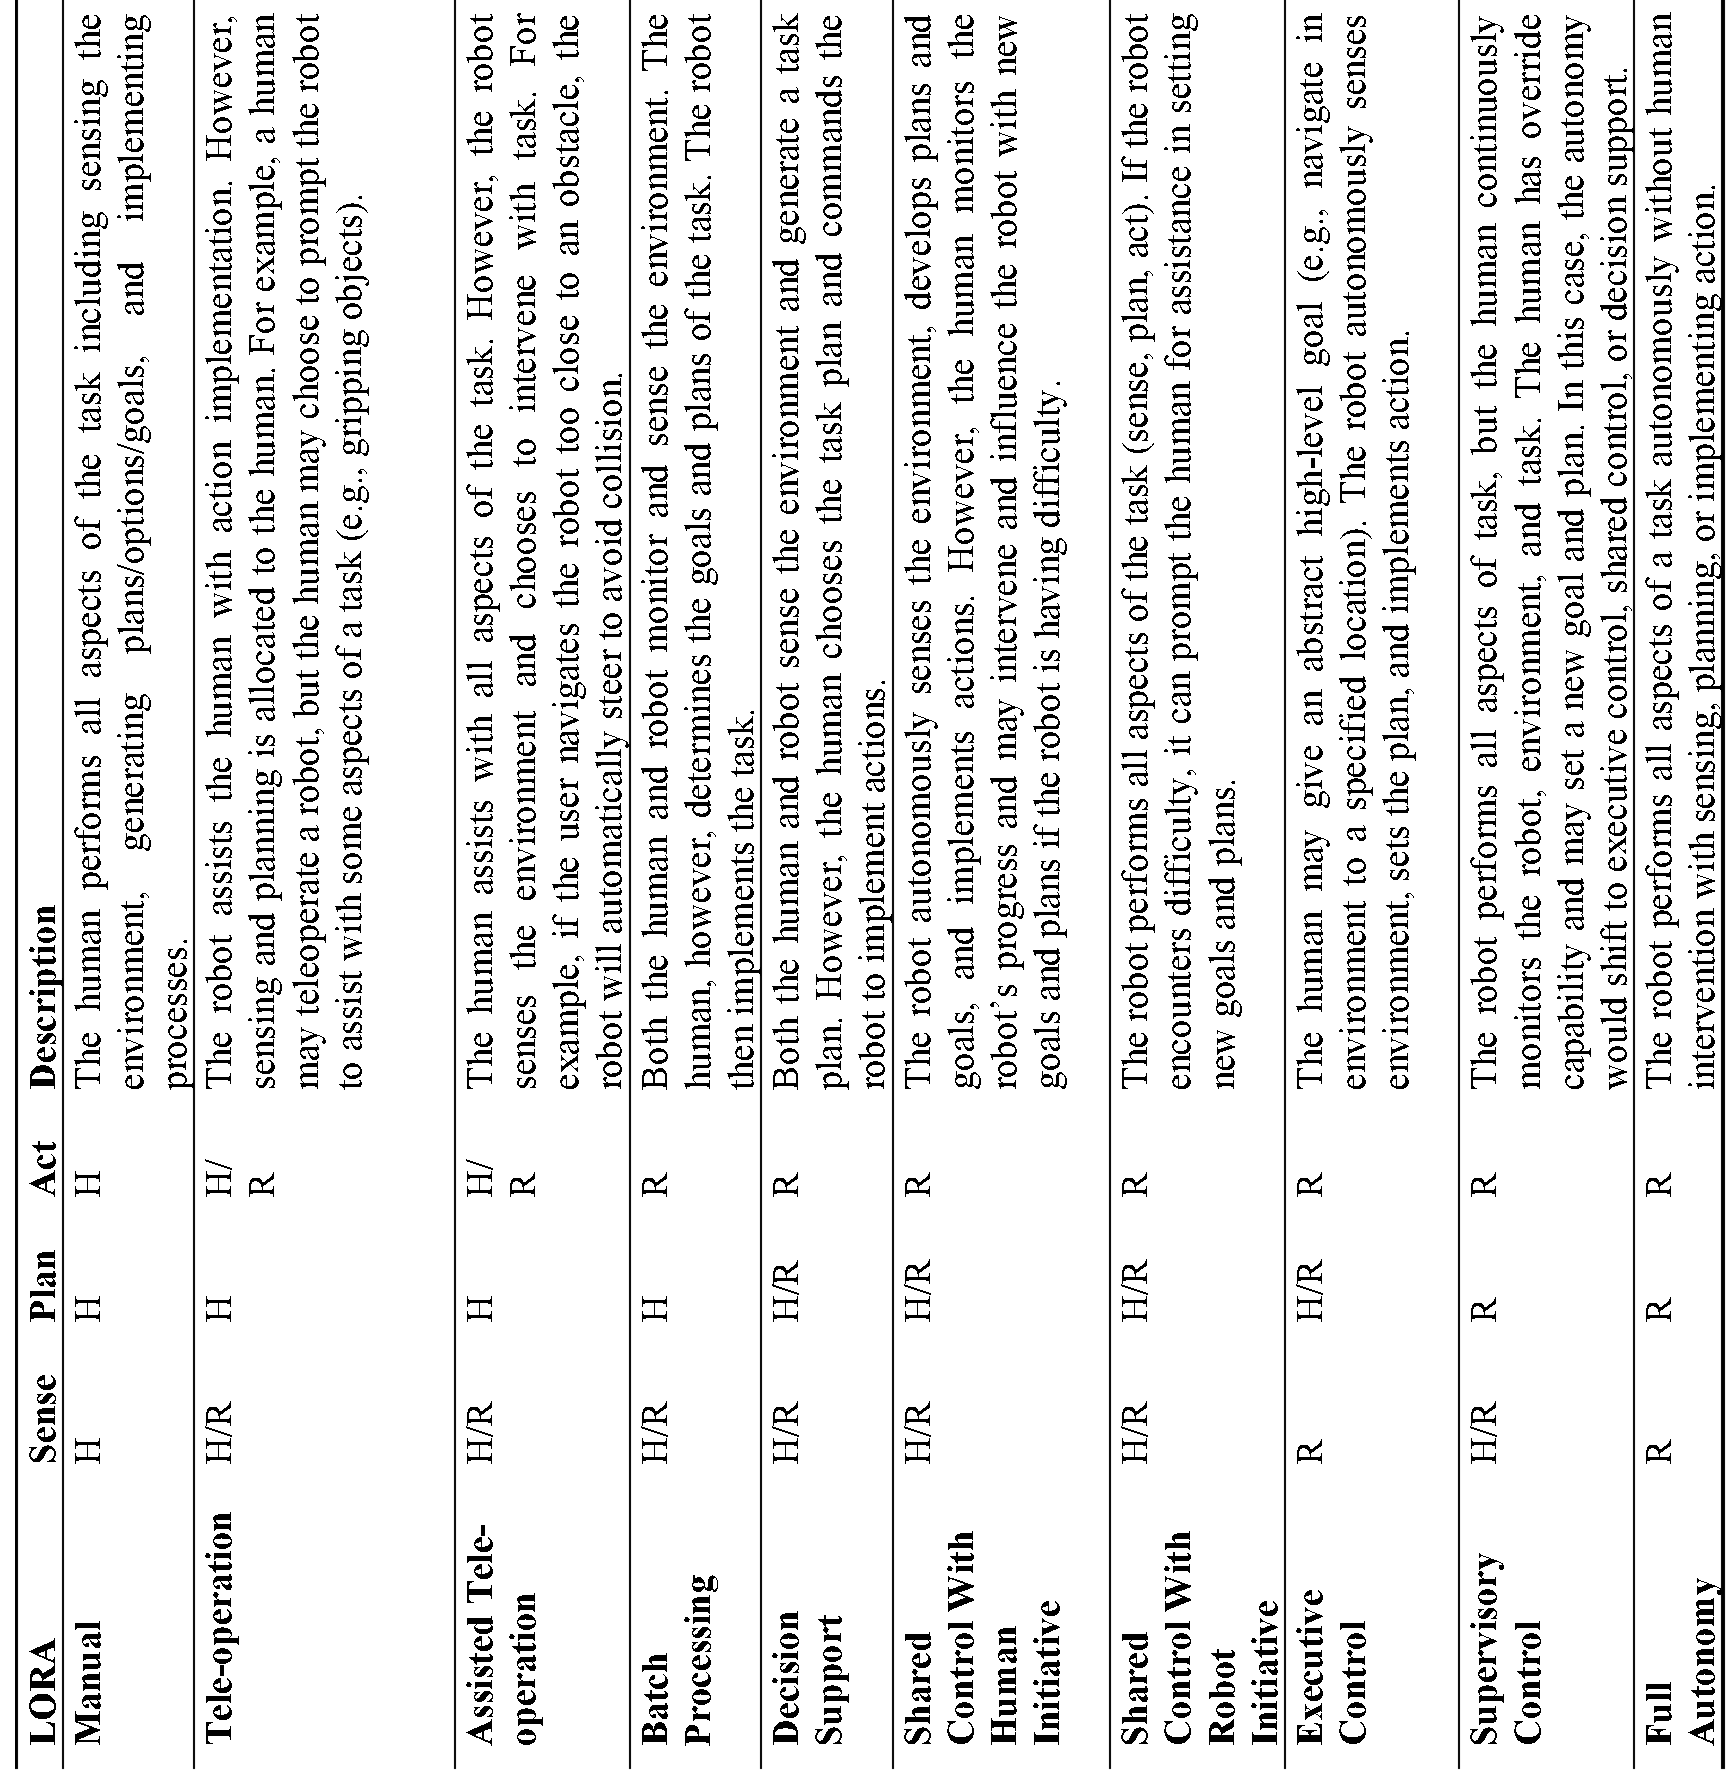
\includegraphics[width=1\columnwidth]{BeerHRItaxonomy.png}
	\caption{The HRI taxonomy proposed by Beer et al.\citep{Beer2014}. Adapted and reprinted from \citep{Beer2014}.} 
	\label{fig:HRItaxonomy}
\end{figure}

%\begin{landscape}
%\begin{table}[]
%	\centering

%		\begin{tabular}{|l|l|l|l|l|}
%			\hline
%			\textbf{LOA}                                  & \textbf{Sense} & \textbf{Plan} & \textbf{Act} & \textbf{Description}                                                                                                                                                                                                                                                               \\ \hline
%			\textbf{Manual}                               & H              & H             & H            & \shortstack{The human performs all aspects of the task including\\ sensing the environment, generating plans/options/goals,\\ and implementing processes.}                                                                                                                                          \\ \hline
%			\textbf{Teleoperation}                        & H/R            & H             & H/R          & \shortstack{The robot assists the human with action implementation. However,\\ sensing and planning is allocated to the human. \\For example, a human may teleoperate a robot, \\but the human may choose to prompt the robot to assist with some \\aspects of a task (e.g., gripping objects).}        \\ \hline
%			\textbf{Assisted teleoperation}               & H/R            & H             & H/R          & \shortstack{The human assists with all aspects of the task. However, \\the robot senses the environment and chooses to intervene with task.\\ For example, if the user navigates the robot too close to an obstacle,\\ the robot will automatically steer to avoid collision.}        \\ \hline
%			\textbf{Batch processing}                     & H/R            & H             & R            & \shortstack{Both the human and robot monitor and sense the environment.\\ The human, however, determines the goals and plans of the task.\\ The robot then implements the task.}                                                                                                                    \\ \hline
%			\textbf{Decision support}                     & H/R            & H/R           & R            & \shortstack{Both the human and robot sense the environment and generate\\ a task plan. However, the human chooses the task plan and\\ commands the robot to implement actions. }                                                                                                                    \\ \hline
%			\textbf{Shared control with human initiative} & H/R            & H/R           & R            & \shortstack{The robot autonomously senses the environment, develops plans\\ and goals, and implements actions. However, the human monitors \\the robot's progress and may intervene and influence \\the robot with new goals and plans if the robot is having difficulty.}                            \\ \hline
%			\textbf{Shared control with robot initiative} & H/R            & H/R           & R            & \shortstack{The robot performs all aspects of the task (sense, plan, act).\\ If the robot encounters difficulty, it can prompt the human for assistance\\ in setting new goals and plans.}                                                                                              \\ \hline
		%	\textbf{Executive control}                    & R              & H/R           & R            & \shortstack{The human may give an abstract high-level goal (e.g., navigate in \\environment to a specified location). The robot autonomously\\ senses environment, sets the plan, and implements action.}                                                                                           \\ \hline
		%	\textbf{Supervisory control}                  & H/R            & R             & R            & \shortstack{The robot performs all aspects of task, but the human continuously monitors the robot,\\ environment, and task. The human has override capability and may set a new goal and plan.\\ In this case, the autonomy would shift to executive control, shared control, or decision support.} \\ \hline
		%	\textbf{Full autonomy}                        & R              & R             & R            & \shortstack{The robot performs all aspects of a task autonomously without human intervention\\ with sensing, planning, or impementing action.}                                                                                                                                                    \\ \hline
		%\end{tabular}
	
%	\caption{My caption}
%	\label{my-label}
%\end{table}	
%\end{landscape}

\subsection{Shared control}
In the robotics community the term "shared control" is often used to generally denote that a robotic system offers some form of collaboration between a human and an AI. In this thesis shared control refers to a specific LOA defined as ``the merging of teleoperation and autonomous control in real time during task execution''~\citep{Backes1994}. In this shared control LOA, input from the operator is blended in real time with the robot's calculated movement in order to produce an improved output. The benefit of using such controllers come mostly in the form of safety and increased accuracy on performing the task. 

Robotic manipulators and arms are able to make the most in terms of performance and safety, with the use of shared control. A study using large-scale industrial manipulators, \citep{Hansson2010} demonstrated that shared control can increase the performance of novice operators compared to pure teleoperation, and decrease the workload in both experienced and novice operators. Similar gains are seen in telesurgery~\citep{Ballantyne2002}. Surgeons' movements are combined with automatic control to produce a more smooth and safe movement (e.g. filtering out hand tremor) for the robotic manipulator. This improves overall safety, gives patients less pain and faster recovery.

An early application of shared control to mobile robots has been in the form of safeguard teleoperation (also known as safe teleoperation). In safeguard teleoperation the operator is driving the robot, but the robot controller reacts in order to prevent commands that are unsafe. Krotkov et al. \citep{Krotkov1996} implemented a safeguard controller to a lunar rover in order to account for time delays between commands. In their field experiments, safeguard teleoperation improved performance and safety in an exploration task. In \citep{Fong2001a} a safeguard controller is proposed for mobile robots deployed in unstructured environments. Urdiales et al. \citep{Urdiales2007} implement a shared control robotic system by coupling the human joystick input with the robot's trajectories based on local efficiency factors. They report improved performance in a navigation task and a more uniform efficiency distribution between participants.

Another mobile robot application that benefits from shared control is robotic wheelchairs. Shared control allows for increased safety without compromising the development of the user's operating skills. Carlson and Demiris \citep{Carlson2010} propose a shared control method which combines safe trajectories from an AI generator with user intention prediction based on joystick commands. They report increased safety when the user is occupied with a distracting secondary task. They also report increased performance in the secondary task. In \citep{Carlson2012}, a human factors evaluation of a shared control wheelchair is presented. Findings based on secondary task reaction time and eye tracking, suggest that shared control results in reduced cognitive workload. Carlson et al. \citep{Carlson2012a} present an adaptive shared control system which modulates the level of assistance based on user's current behaviour. They report increased performance and increased user acceptance. Research from Parikh et al. \citep{Parikh2005} reveals that users also tend to prefer shared control compared to teleoperation and autonomous control, when operating a robotic wheelchair.

\subsection{Traded control}
Another common approach to variable autonomy is the switch between the two extremes in the LOA scale (i.e. pure teleoperation and autonomy). This is called traded control. Such an approach aims at using autonomy in tasks that the robot is capable of performing but can be tedious or difficult at times for the operator. Teleoperation is used in the tasks that the robot is not able to perform. This approach constitutes the base of our research. However, as we will describe in a later section, our research tackles some profound questions such as how to trade control dynamically, when and why (i.e. based on some factors). Here we present a brief overview of traded control.

Kortenkamp et al. \citep{Kortenkamp2000} present an architecture for traded control in which the robot queries the operator each time it finishes a simple action. Mano et al. \citep{Mano2009} constructed a traded control system for SAR. They heuristically define situations that will make use of autonomy mode and situations that will use teleoperation. These heuristics are based on the task and the operation environment (e.g. presence of obstacles, wireless communication quality). However, they do not address how the switch will take place and who has the responsibility for triggering the switch. A principled way of trading between teleoperation and autonomy is investigated in \citep{Sellner2005}. Robots in an assembly scenario query the operator about trading control after a model-based cost-benefit analysis. Human and robot performance models are explicitly trained by repeating the assembly scenario several times. Lastly, a control architecture is created \citep{Kim2004} to be used in an underwater robotic vehicle. This architecture allows operators to switch between teleoperation and semi-autonomous operation, in which a human supervisor is giving commands at the mission level.

\subsection{Multiple levels of autonomy}
Research on variable autonomy also considers robotic systems that implement several LOAs. In such cases the distinction between levels is less clear, e.g. safe teleoperation is used as a different LOA from shared control. Commonly four LOAs are implemented: a) teleoperation in which the operator has full control; b) a safe  mode in which the operator teleoperates the robot but the robot can take initiative to protect itself; c) shared control (as above); and d) an autonomous or semi-autonomous mode in which the operator gives high level commands to the robot (e.g. specific goals). The operators are able to switch between these modes mostly based on their own judgment. A typical example is the system in \citep{Bruemmer2002}. A mobile robot is presented which is capable of switching between different levels of autonomy at the operator's command. The system aids operator's judgment by providing on-screen indications of blockage or motion resistance. More research on multiple LOAs will be presented from this project's perspective later on.


\section{Dynamically switching levels of autonomy}
The use of different LOAs leads to a series of open challenges. Which LOA should be used under which conditions?; who should initiate switches in the LOA and based on which factors?; and how can we investigate the trade-offs offered by switching LOAs in a repeatable manner?

The majority of the robotics literature is focused on describing the engineering and/or computational details of new technologies, while comparatively few studies address the issues of rigorously evaluating how well a human can use such robots to carry out a real task. Additionally, the autonomous robotics literature has historically tended to be somewhat separated and distinct from the literature investigating the issues of teleoperation, with relatively little work specifically focusing on variable autonomy systems.

Research which focuses on investigating dynamic LOA switching on mobile robots is fairly limited. Furthermore, the investigation of Mixed-Initiative (MI) systems to address this dynamic switching is even more limited, as highlighted by Jiang and Arkin \citep{Jiang2015} and by publications arising from this thesis, e.g. Chiou et al. \citep{Chiou2015}. A large part of the literature, e.g. \citep{Krotkov1996, Bruemmer2005}, is focused on comparing the relative performance of separate LOAs, and does not report on the value of being able to switch between LOAs. In contrast, our work specifically addresses the issues of dynamically changing LOA on-the-fly (i.e. during task execution) using either a MI or Human-Initiative (HI) paradigm. 

In this section, research addressing the strategies for switching autonomy levels is discussed. More specifically, the discussion aims at pointing out the gaps in the literature regarding three key aspects: a) conducting rigorous experiments using a principled scientific framework; b) LOA switching initiated by the human operator (namely HI); and c) LOA switching initiated both by the AI or/and the operator (namely MI). 

In contrast to the literature presented here, and to the best of our knowledge, our work is the first that exploits rigorous methodologies from psychology and human factors research to carry out a systematic study of variable autonomy in mobile robots; the first mobile robot experiments that combine quantifiable and repeatable degradation factors for both human and robot; and the first work which formally and systematically evaluates the benefits of combining the capabilities of both human and autonomous control in the context of dynamically mode-switching systems. 

\subsection{Conducting variable autonomy experiments}\label{section:framework_lit}
Surprisingly, previous research on variable autonomy in mobile robots lacks a rigorous experimental framework that will allow for meaningful and repeatable scientific inference. Characteristically much of the published experimental work does not carefully control for possible confounding factors. These factors can vary from partially uncontrolled test environments (as in \citep{Marble2004}), up to the absence of standardized training for human test-subjects as in \citep{Bruemmer2005,Few2006, Bruemmer2004}. It is particularly important to control for the training and experience of human test-subjects, as these factors are known to affect overall robot operating performance \citep{Bruemmer2008, Armstrong2015}. Additional confounding factors include the robot having different speed limits in the different conditions tested \citep{Few2006}, or different navigation strategies of human operators like the ones observed in our work \citep{Chiou2015}. In contrast to our work, Nielsen et al.~\citep{Nielsen2008} report no significant primary task results due to large measurement variances, but they do present a method for systematically categorizing the different navigational strategies of human operators.  

All of the papers discussed above make important contributions in their own right, and we do not intend to devalue such work in any way. However, across the related literature we note a deficiency of: a) rigorous statistical analysis; b) clarity on assumptions and hypotheses; c) precise and detailed descriptions of the experimental protocol followed; d) a formalized, coherent and repeatable experimental paradigm. In contrast, in disciplines such as psychology and human factors, the above criteria constitute standard practice.

An excellent example of related work, which does provide a rigorous protocol, statistical analysis and detailed description, is the work of Carlson et al. \citep{Carlson2012a}. They validate an adaptive shared control system, while degrading task performance with the use of a secondary task. However, their work is focused on the use of a Brain-Computer Interface for robot control. Because this field is relatively young, and the problems are extremely difficult, \citep{Carlson2012a} used a robot navigation task which was comparatively simplified, i.e. operators only control left-right movement of a robot using a keyboard. 

\subsection{Human-Initiative variable autonomy}
\label{section:HI-background}
A Human-Initiative (HI) variable autonomy system, is a system in which the human operator can dynamically switch between the different LOA (e.g. teleoperation and autonomy) (see publications arising from this thesis \citep{Chiou2016}). In such systems only the human operator has the authority to initiate LOA switches based on his/her judgment. This judgment is often aided by suggestions made by the AI. The robot adopts a passive role without any kind of authority to initiate a LOA switch. This can be problematic in cases where the operator's judgment is impaired, e.g. if they have incomplete situation awareness (SA). Also it can be possible that the operator simply does not realize that a change in LOA is possible or beneficial (e.g. when under high workload). Additionally, the task of considering whether to switch LOA can add extra workload to the operator. 

In \citep{Goodrich2001} a system is presented with different LOAs. However, the initial LOA choice cannot change on the fly. Building on \citep{Bruemmer2002}, Baker and Yanco \citep{Baker2004b} presented a robotic system in which the robot aids the operator's judgment by suggesting potential changes in the LOA. However, the system was not validated experimentally. Marble et al. \citep{Marble2004} conducted a SAR-inspired experiment in which, similar to our experiments, participants were instructed to switch LOA in order to improve navigation and search task performance. However, \citep{Marble2004} was intended to be a usability study which explored the ways in which participants interacted with each different LOA. In contrast, our own work is additionally focused on evaluating and demonstrating the overall task-performance when LOA levels can be dynamically switched. As in our own work, \citep{Marble2004} also incorporate secondary tasks into their experiments. However, in contrast to our work, the use of these secondary tasks was opportunistic in nature because participants were only instructed to perform them optionally. Hence, the secondary tasks in \citep{Marble2004} do not degrade human performance on the primary task (steering the robot). Also, unlike our work, \citep{Marble2004} did not incorporate any methods into their experiments for degrading the robot's autonomous performance in a controlled way. In \citep{Ibanez-Guzman2004}, a robot was presented which could navigate autonomously to way-points specified by a human operator. This paper suggested that the performance of such robots might be improved by enabling a human operator to teleoperatively intervene in situations such as navigating narrow corridors, where the authors anecdotally reported difficulties with autonomous navigation. However, performance of this system was not experimentally validated in \citep{Ibanez-Guzman2004}.

Although it is out of this thesis scope, variable autonomy research in the field of multiple robots being controlled by a single operator, provides similar studies. However much of this research (e.g. \citep{Hardin2009,Goodrich2007b}) is focused on higher levels of abstraction than our work, e.g. planning or task allocation. Other experiments, e.g \citep{Riley2006, Valero-Gomez2011}, are focused on human factors issues such as gaining SA when controlling multiple robots, or how the operator interacts with as many robot as possible.


\subsection{Definition and taxonomy of Mixed-Initiative control}
\label{section:MI-taxonomy}
In \citep{Jiang2015} Jiang and Arkin present an elaborate definition of MI control in the context of human-robot teams. They define MI as:

\begin{quotation}
	"A collaboration strategy for human-robot teams where humans and robots opportunistically seize (relinquish) initiative from (to) each other as a mission is being executed, where initiative is an element of the mission that can range from low-level motion control of the robot to high-level specification of mission goals, and the initiative is mixed only when each member is authorized to intervene and seize control of it."
\end{quotation}

They also present the first taxonomy for MI robotic systems. Their taxonomy has three dimensions: 

\begin{itemize}
	\item \textbf{Span-of-mixed-initiative} which characterizes the control elements (initiatives) in which both agents are capable of initiating actions.
	
	\item \textbf{Initiative reasoning capacity} which characterizes the ability of an agent to reason about taking the initiative.
	
	\item \textbf{Initiative hand-off coordination} which characterizes the strategies used by the system when shifting initiative from one agent to the other.
\end{itemize}

Regarding the span-of-mixed-initiative, our system presented in Chapter \ref{chapter5:MI} is \textit{mostly-joint} as both agents have initiative capacity over two of the control elements, navigation execution and LOA switch. Regarding the initiative reasoning capacity, the system is characterized as \textit{deliberative}. It has the ability to reason about initiating actions deliberately based on an online performance metric and simplified context awareness. Lastly, the initiated actions are communicated explicitly to the agents via the control interface and sound notifications. Thus, in the initiative hand-off coordination dimension our system is characterized as \textit{explicitly-coordinated}.

\subsection{Mixed-Initiative control related systems}
\label{section:MI-systems}
Our literature survey found several systems characterized by authors as MI. However given the comprehensive taxonomy in \citep{Jiang2015}, we believe that many of them cannot be characterized as truly MI control systems. This is due to the fact that the human-robot team does not share any initiatives, e.g. in \citep{Finzi2005} only the operator is initiating actions based on system's suggestions. In this survey we will only present systems that have some form of true MI control.

Shared control is a widely researched LOA falling under the banner of MI control. Any mixed-initiative is restricted inside the shared control LOA. This means that the robot will only take initiative to blend its navigation control input with the one from the operator, in order to improve the control output. Similarly, in safeguard teleoperation (another form of shared control), the robot initiative takes place reactively to prevent collisions. In both cases no LOA switching takes place.

Nielsen et al. \citep{Nielsen2008} conduct experiments using multiple LOAs. However, the LOA is chosen during the initialization of the system and cannot change on the fly. Moreover, similar to shared control, the robot has only reactive initiative inside a specific LOA to prevent collisions. Lastly, initiative is not coordinated by any hand-off strategy. Multiple robotic configurations using multiple LOAs (teleoperation, safe mode, shared mode, autonomy) are tested in \citep{Bruemmer2005}. In shared mode the robot drives autonomously while accepting interventions from the operator. In safe mode the robot takes initiative only to prevent collisions. However, these LOAs cannot change on the fly and robot's initiative is limited in safe mode. Few et al. \citep{Few2006} present a control mode in which the operator is giving directional commands to adjust robot's navigation by using the joystick. The system offers limited initiative which depends on the frequency of operator's interaction.

Research on MI systems that are able to switch LOA dynamically or have initiative capabilities not restricted to a specific LOA, is fairly limited. Moreover, the MI systems proposed are either theoretical or not experimentally evaluated.  Bruemmer et al. \citep{Bruemmer2003b} present a theoretical multiple LOA, MI system. This system is based on "the theory of robot behavior" (human understanding of the robot) and  "the theory of human behavior" (robot understanding of the human). The latter proposes the use of readily available non-intrusive workload cues from operator as an indication of poor performance. More specifically, it proposes the use of the frequency of human input and the number and kind of dangerous commands issued by the operator, as performance indicators. This provides the robot with the capacity to initiate switches between the different LOAs. However, it can be argued that input frequency is not necessarily an indication of poor performance. Rather it reflects different operators' driving styles. Adams et al. \citep{Adams2004} propose a MI robot control architecture which relies on the detection of operator's emotional state. Initiative is mixed in all the levels of the system, i.e. in setting goals and constrains, planning and execution. Changes in control are initiated based on the operator's sensed state (e.g. boredom, stress, drowsiness, engagement). This requires user-specific models that can be challenging and impractical to create. Having a working system that mixes initiative in all the levels of abstraction is an extremely challenging concept for the current state of the research. Lastly, in contrast to our work, \citep{Adams2004} does not propose any hand-off coordination strategies and the system is not experimentally evaluated.

In studies of multi-robot systems, variable autonomy often lies on a higher level of abstraction compared to our work. Manikonda et al. \citep{Manikonda2007} describe a multi-robot MI controller and testbed for human-robot teams in tactical operations. The agents in the system share information towards a common model of the world and other agent's behavior. Based on this information they are able to initiate modifications to their goals and associated roles in the team. In \citep{Hardin2009} a MI approach is proposed in a multi-robot search task. Robots are equipped with the ability to initiate changes in their respective search areas (e.g. size of search area). These changes are reactively triggered by specific events, e.g. the human operator has identified an item of interest.

In summary, MI robotic systems found in the literature offer limited initiative inside a predefined LOA. In the case of multiple robots, the MI lies in a higher level of abstraction, making assumptions about other layers, e.g. navigation. Moreover, contrary to our work, initiative actions from the robot are not based on task performance metrics. The robot controller is rather taking initiative by reacting to sensor input (e.g. obstacles).

To the best of our knowledge, our work is the first to use an online task performance metric to address the problem of switching LOA during task execution using a MI controller. Also we are the first to show in a systematic way the benefits to human operator cognitive workload and the benefits to different tasks performance (e.g. navigation, spacial awareness tasks etc) of a robotic system that initiates dynamic LOA switches. 

\subsection{Human-Robot Interaction with LOA switching robots}\label{section:HRI_LOA_switch}
As seen in the previous sections and in our work in \citep{Chiou2015}, research which focuses on investigating dynamic LOA switching on mobile robots is (perhaps surprisingly) very limited. Furthermore, very little previous literature has attempted to rigorously evaluate variable autonomy systems which are able to switch LOA on-the-fly, as shown in our work \citep{Chiou2016}. Consequently, human interaction with a variable autonomy system remains predominantly unexplored in the prior literature. Studies which address similar applications to ours, e.g. SAR, have evaluated how operators interact with user interfaces~\citep{Yanco2004,Baker2004}. Other studies explored the human operator's interaction with the robot in order to exchange information~\citep{Fong2003}, but did not explore issues of control. Other studies investigated the human operator's interaction with a robotic system, but were restricted to exploring a single LOA~\citep{Bruemmer2005}, and did not explore the issues of variable LOA. Interesting studies of robotic wheelchairs, which exploited autonomous navigation capabilities by using a shared control (mixed initiative) architecture, measured the interaction of the operator with the collaborative control system based on joystick activity~\citep{Carlson2008}. In contrast to the above literature, this thesis specifically investigates issues of the interaction of a human operator with a variable autonomy (multiple LOAs) system.

In \citep{Baker2004b} a system was presented which aids the operator's judgment by automatically suggesting potential changes in the LOA. However, unlike our work, no data were presented on the operator's interaction with this LOA switching controller, because the system was not validated experimentally. As seen in Section \ref{section:HI-background}, the collaborative control for the robot presented in \citep{Ibanez-Guzman2004} was not experimentally validated and thus no HRI was presented. Marble et al.~\citep{Marble2004} conducted a SAR-inspired experiment in which participants were instructed to switch LOA in order to improve navigation and search task performance. In contrast to our work,~\citep{Marble2004} did not investigate the human operator's interaction with the a robotic system in which LOA levels can be dynamically switched. 

To the best of our knowledge and in contrast to the literature reported here, our work is the first on mobile robots that reports a systematic analysis of the ways in which human operators interact with, and exploit the capabilities of, a robotic system in which LOA can be dynamically switched either by the operator or both by the AI and the operator.

\section{Measuring and inducing cognitive workload}
\label{chapter2:workload}
Cognitive workload is one of the major reasons of performance degradation in humans when conducting a task. As discussed in Section \ref{section:HRIfield}, robot operators often suffer from errors and performance degradation due to workload. Thus, inducing and measuring workload is of importance when evaluating variable autonomy robotic systems.

Various methods exist for measuring workload. These methods can be categorized in three main classes \citep{Farmer2003}: physiological measures; subjective measures; task performance measures. In this section each of them is briefly discussed. 

\subsection{Physiological measures}
Physiological measures are based on the assumption that workload will cause a physical reaction to the body of the person experiencing it. Such measures include respiratory activity, heart rate, brain activity, eye blink, eye movement and pupil dilation. They are direct objective measures and non-intrusive in regard to the task. However, they significantly raise the complexity of experiments and data analysis. The data are hard to collect; often require specialized equipment or processing; and are prone to noise. For these reasons, physiological measures have not been used in this work.

An example of a physiological measure that offers promising potential is Electroencephalography (EEG). EEG measures the electrical activity of the brain with electrodes placed in standardized positions in the scalp. It has been successfully used as an on-line measure of workload and validated in many studies \citep{Wilson2007,Wilson2003,Wilson2000,Kothe2011,Prinzel2003}. Compared to other physiological measurements it has three key advantages: a) offers much better temporal resolution on the order of milliseconds; b) there are evidence that EEG outperforms some of the other techniques for measuring workload on-line \citep{Wilson2003a}; c) it is a measure of brain activity and as such can potentially provide much more information regarding the cognitive state of the operator than just workload. The latter makes EEG very appealing as an input to adaptive automation. For example EEG can be used on the operator to determine if a stimulus has being perceived \citep{Wyble2006a}, recognize emotions \citep{Schaaff2009} or measure task engagement \citep{Berka2007a}. Disadvantages of EEG include the fact that the signal is prone to artifacts (e.g. created by perspiration or movement) and noise and thus has to be recorded with care. Also, it has day to day variability \citep{Christensen2012} and highly depends on the individual. Hence, is not easy to generalize.

\subsection{Subjective measures}
Subjective measures come in the form of questionnaires and are the easiest and least intrusive methods to investigate workload. Participants, after the experiments, are asked to rate the workload they experienced in one or more scales. Thus, subjective measures cannot provide real-time assessment of workload. Also they are highly subjective as they capture the individual differences between operators. 

Such measures have been used extensively throughout the experiments in the form of NASA Task Load Index (NASA-TLX) \citep{Hart1988}. It is the most popular and well validated technique \citep{Hart2006} of subjective workload measurement. It rates perceived workload in order to assess a technology or system. NASA-TLX is considered a standard in the relevant human factors or teleoperation studies. It is multidimensional as it attributes workload to the following factors: Mental; physical; temporal demands; frustration; effort; performance. It applies a weighting scheme in order to decrease the variability between different participants. However, in our experiments we used what is called "raw NASA-TLX", which is simply a NASA-TLX without the weighting scheme. Raw NASA-TLX was found to be equally accurate, although there is an ongoing debate about its use \citep{Hart2006}. The reason the raw version was used, is that the weighting scheme can be tedious and time consuming for participants as it requires responses to a number of pairwise comparisons between the workload factors. These reasons, as observed during our pilot studies, led some of the participants to respond randomly in the pairwise comparisons.

This leads to participants answering in random some of the pairwise comparisons of the weighting scheme, as observed during our pilots experiments.

Lastly, Yagoda \citep{Yagoda2010} proposed a workload questionnaire to be used in conjunction with NASA-TLX in order to provide more insight on specific HRI factors that affect workload (e.g. team process). This technique is new and not validated to the best of our knowledge. Hence it has not been used. 

\subsection{Task performance measures}
Task performance workload assessment is done by measuring the performance on a primary or a secondary task. The assumption behind measuring workload with this method is that humans have limited cognitive resources. Thus, performance on a secondary or on the primary task are an indication of workload and will degrade with difficulty.

Our experimental paradigm uses a secondary task in order to primarily induce and secondary to measure operator's workload. Thus, the secondary task must be relevant and mentally interfere, but not interact, with the primary task. According to the Multiple Resource Theory \citep{Wickens2008,Wickens2002} this happens when two or more tasks share the same resources. For example the same perceptual modality and/or the same processing stages. The primary task of operating a robot through an interface, is mainly visual and involves spatial reasoning. Hence the secondary tasks used in the experiments are visual and/or require some sort of spatial reasoning. 


\chapter{TOWARDS THE PRINCIPLED STUDY OF VARIABLE AUTONOMY}\label{chapter3:towards}

Conducting experiments in any field requires a rigorous scientific framework for yielding meaningful, repeatable, and statistically validated results. Our literature survey, as reported in Section \ref{section:framework_lit}, discovered the absence of a variable autonomy experimental framework. Thus, our first step was towards defining such an experimental paradigm by conducting an exploratory pilot experiment.

This chapter is based on our Systems, Man, and Cybernetics conference paper \citep{Chiou2015}. It describes a pilot experiment in which a variable autonomy robot completes a navigation task. It explores the comparative performances of the human-robot system at different autonomy levels under different sets of conditions. Sensor noise was added to degrade robot performance, while a secondary task induced varying degrees of additional workload for the human operator. Carrying out these experiments and analyzing the results has highlighted the profound complexities of designing tasks, conditions, and performance metrics which are: principled; eliminate confounding factors; and yield scientifically rigorous insights into the intricacies of a collaborative system that combines both human and robot intelligences. The main contribution of this chapter is the description of lessons learned from attempting this experiment, and a variety of suggested guidelines for other researchers to consider when designing experiments in this context. Lastly, these lessons and guidelines, informed a framework for the systematic development and validation of a system for changing LOA on the fly. This framework was used at the later experiments as it enables for more robust and clean experimental designs.

\section{System description}\label{chapter3:system}
Our experimental system used a Pioneer-3DX mobile robot equipped with a laser range finder sensor and a camera (see Fig. \ref{fig:pioneer_exp1}). Remote control was achieved by a wireless link to the Operator Control Unit (OCU) which comprised a laptop connected to a screen showing the control interface (see Fig. \ref{fig:interface_pilot}) along with a joystick and a mouse. There is a rich literature on standards and guidelines for designing interfaces as seen in Section \ref{section:interfaces_lit}. The interface of our system adopts these recommended standards and guidelines where possible. Note that the intention of this work was not to design a better interface, but to explore the performance variations of human versus autonomous control under various conditions. 

\begin{figure}
	\centering
	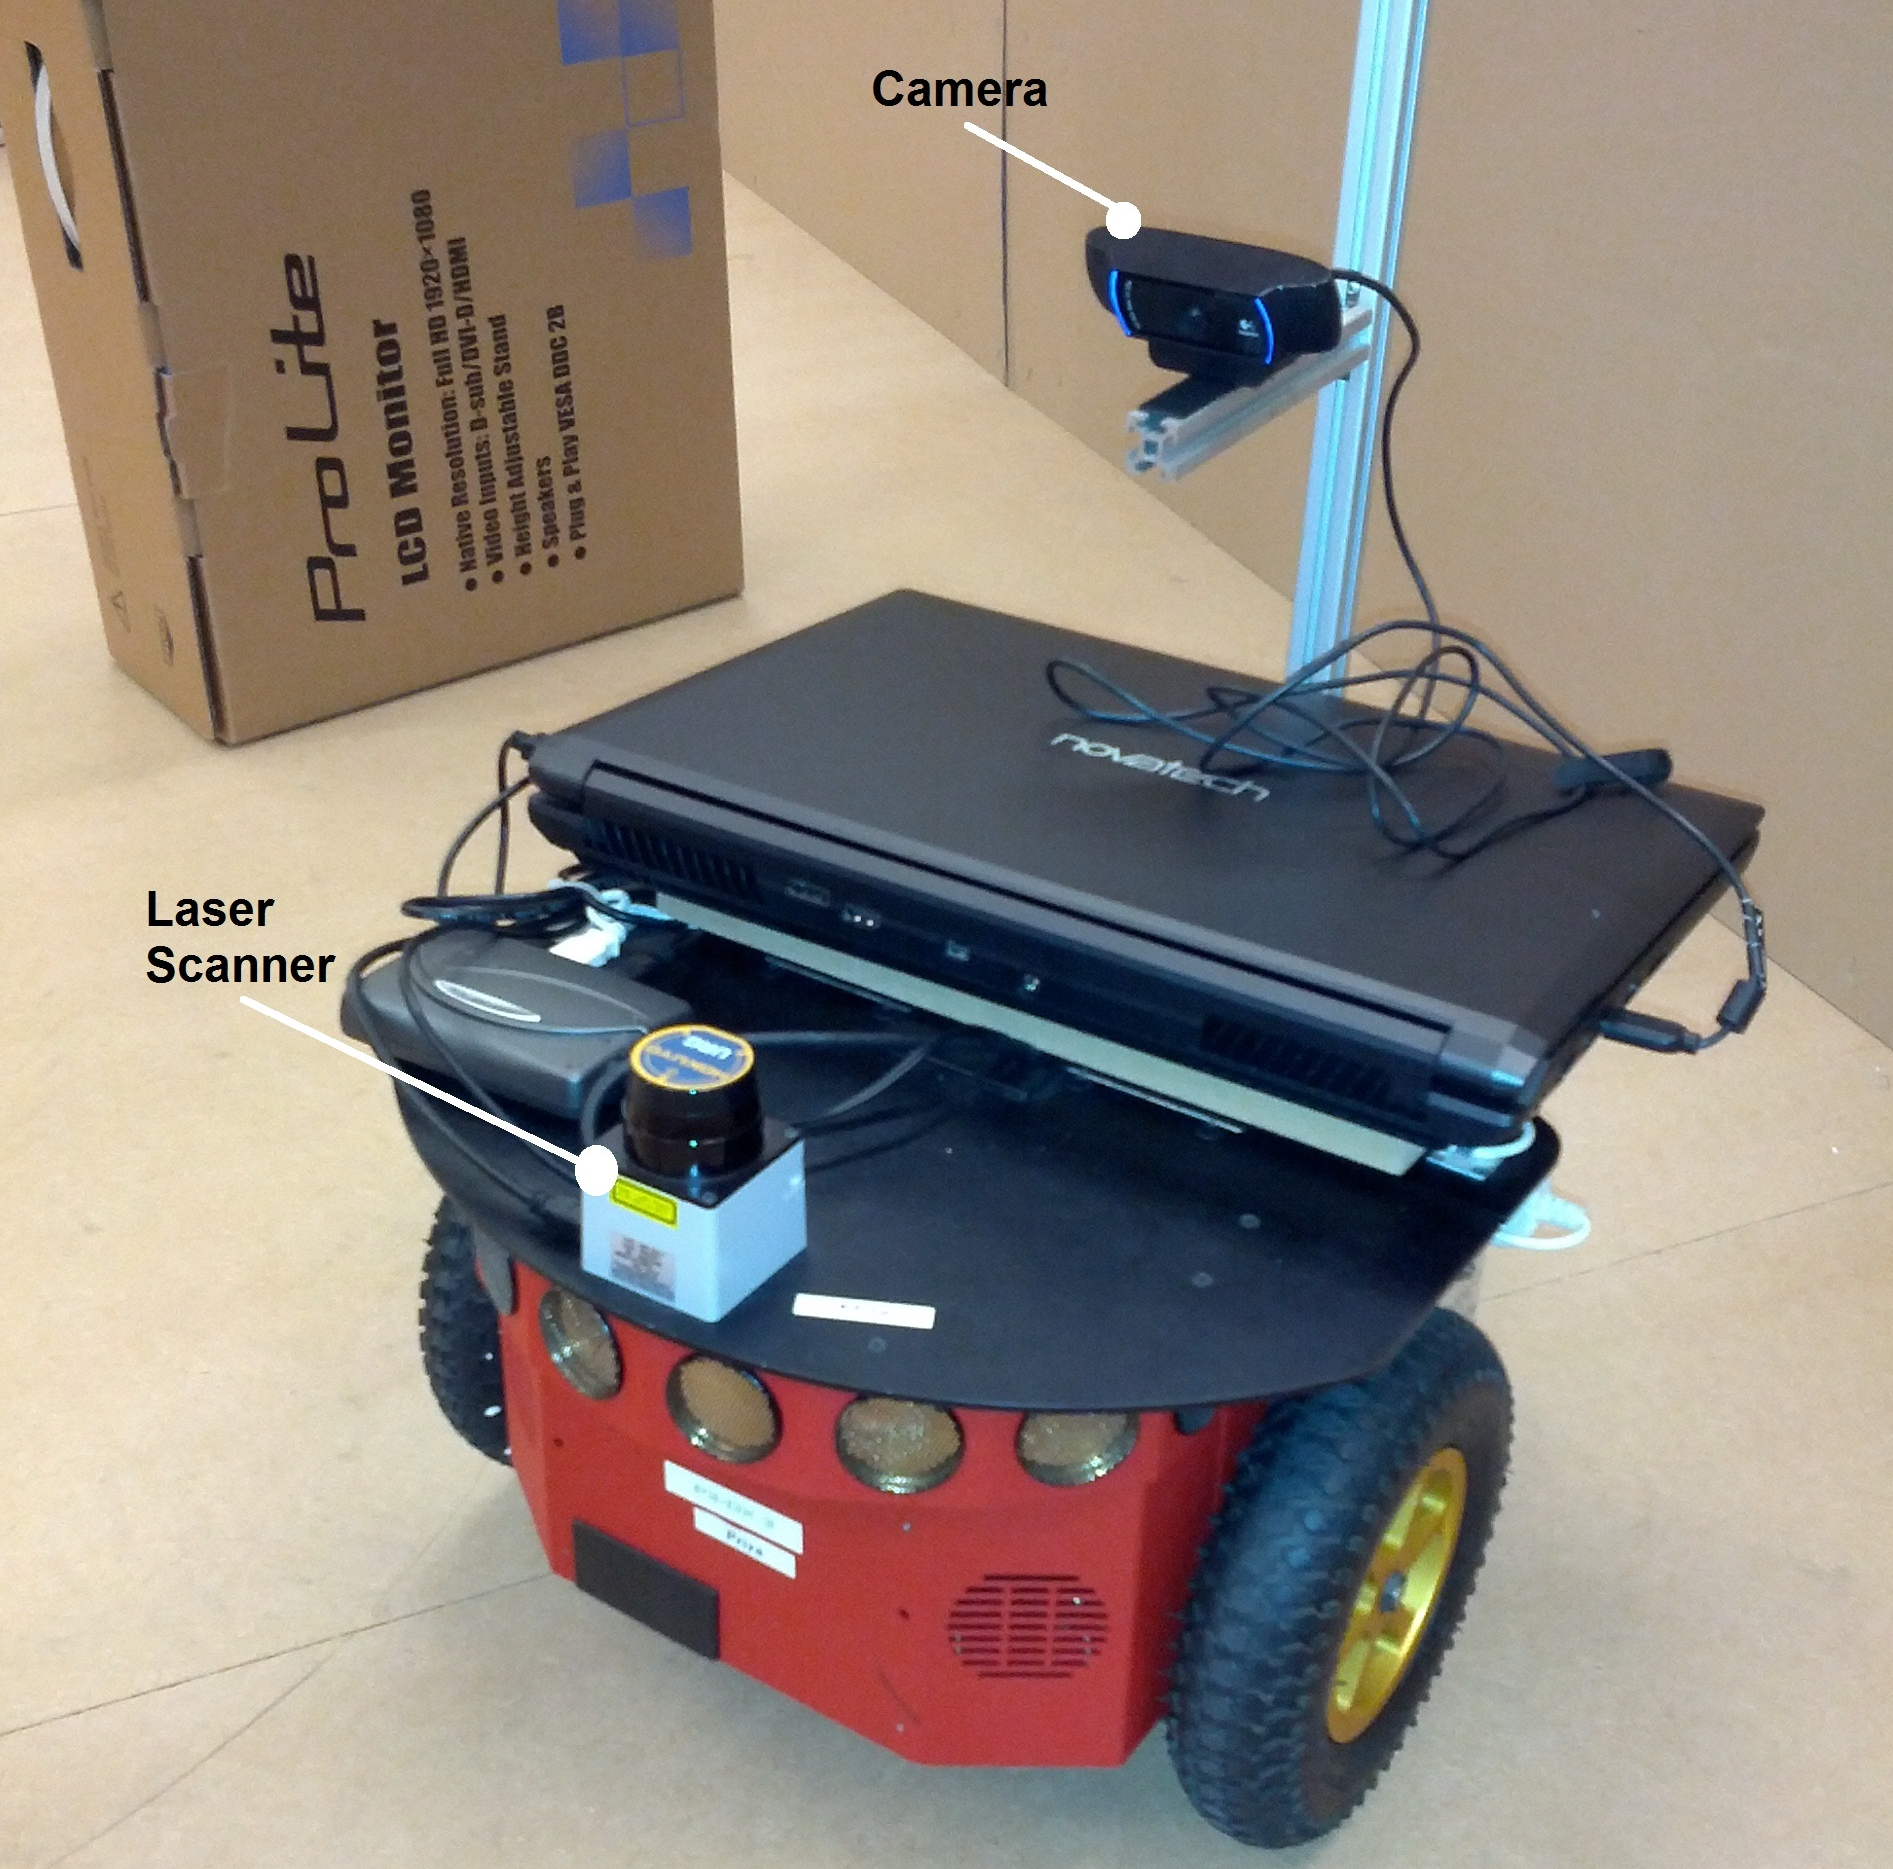
\includegraphics[width=0.5\columnwidth]{chapter5_fig/pioneer.jpg}
	\caption{The pioneer-3DX robot used in the experiment, equipped with a laser range finder and a camera.}
	\label{fig:pioneer_exp1}
\end{figure}

\begin{figure}
	\centering
	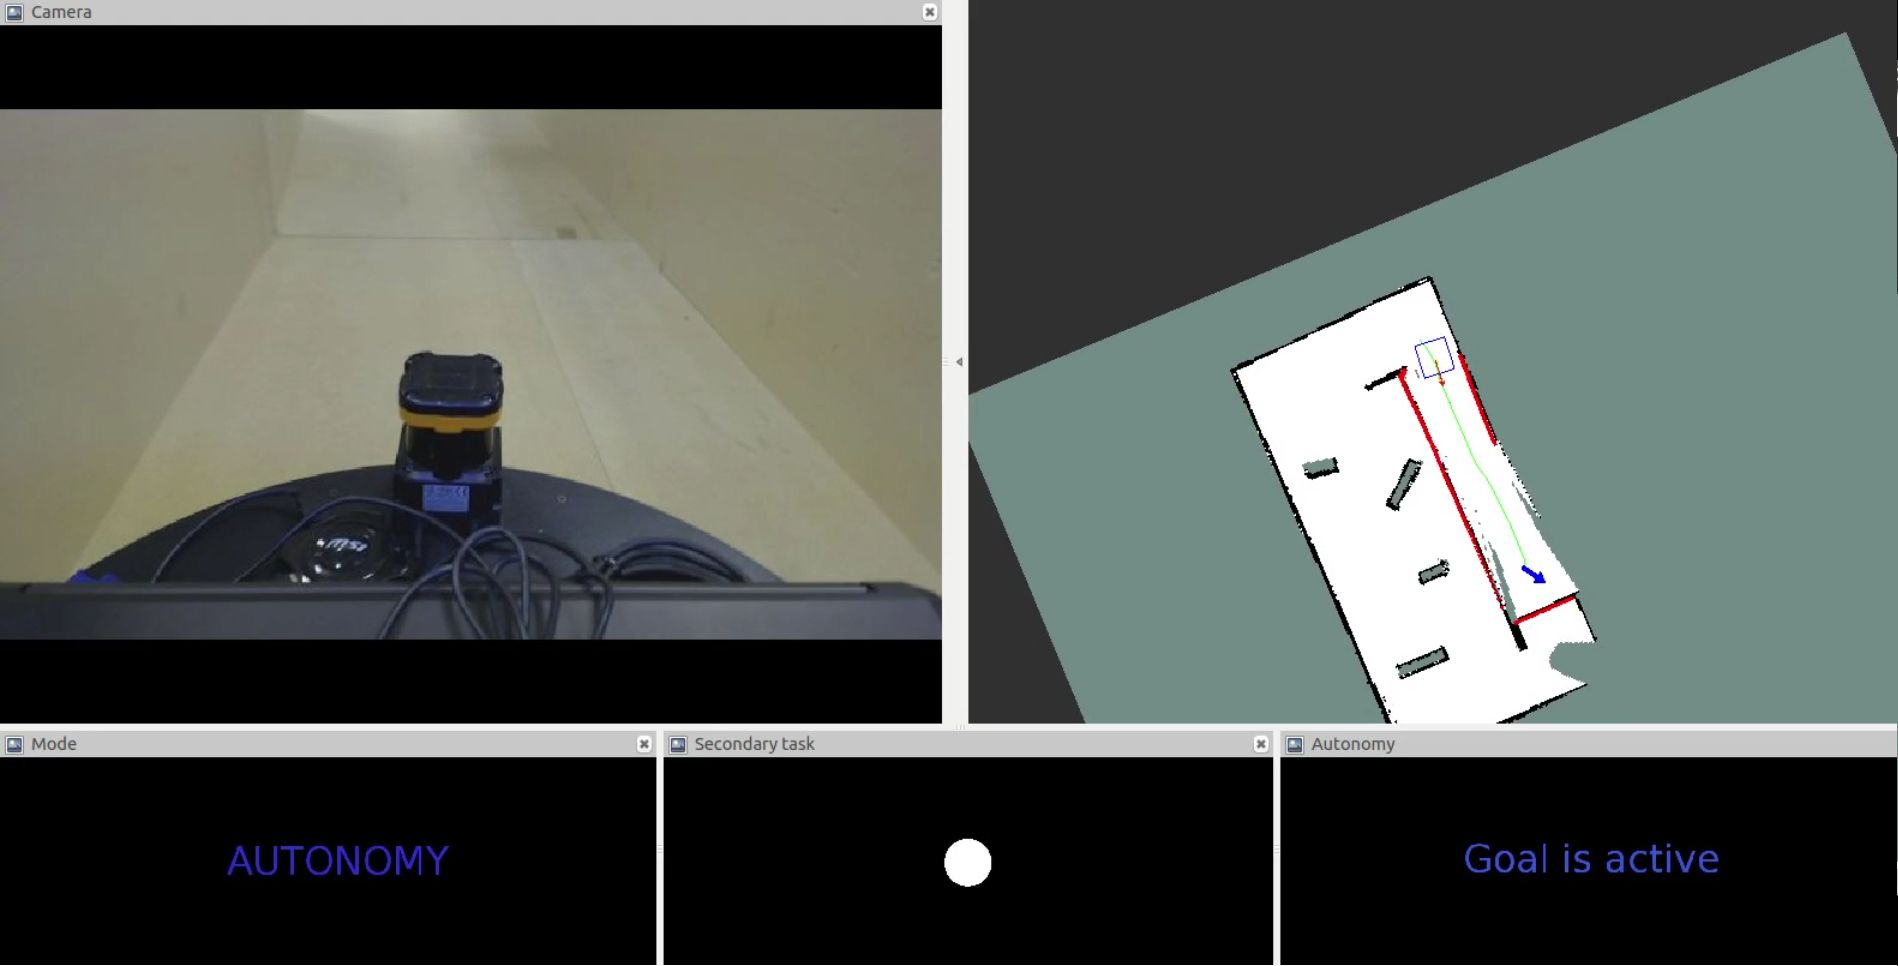
\includegraphics[width=1\columnwidth]{chapter3_fig/interface_pilot.jpeg}
	\caption{The control interface as presented to the operator. \textbf{Top}: video feed from the camera and the map of the environment. Inside the map, the position of the robot is visualized by the 3D model, the current goal by the blue arrow, the AI planned path by the green line, the obstacles' laser reflections by red and map walls with black. \textbf{Bottom}: the current autonomy mode, secondary task, and the status of the robot. }
	\label{fig:interface_pilot}
\end{figure}

Our system offers two LOAs: \textbf{Teleoperation:} the human operator drives the robot with the joystick, while gaining SA via a video feed from the robot's onboard camera. Additionally a 2D map generated by Simultaneous localization and Mapping (SLAM) using the laser, is displayed on the OCU. \textbf{Autonomy:} the operator gives high level navigation commands to the robot, which is responsible for executing them autonomously. The commands consist of the human operator clicking a desired destination on the 2D map. The robot autonomously navigates towards these destinations. The operator can switch between the two modes of operation at any time by simply using their chosen control method.

The system was developed in Robot Operating System (ROS). For autonomous navigation ROS's \textit{navigation stack} was used. It is a robust state-of-the-art solution \citep{Marder-Eppstein2010}. For SLAM the \textit{OpenSlam's GMapping} algorithm \citep{gmapping} through the ROS wrapper package called \textit{slam gmapping} was used. Other in-house developed ROS software is responsible for teleoperation, LOA switching and providing information to the interface which is an adapted version of ROS  \textit{rviz} package.

\section{Pilot experiment}
\label{section:chapter3-pilot}
Two main hypotheses guided the design of this experiment and the design of the experiments presented in later sections. These two hypotheses are:

\begin{enumerate}
	\item The factors that affect operator's performance are cognitive workload and fatigue.
	\item The factors that affect robot's performance are: a) the uncertainty in information given (i.e. sensing) to an AI algorithm; b) the limited capabilities of an AI algorithm to process the given information; c) the complete absence of a capability specific algorithm (e.g. computer vision detection of victims in SAR) and thus the absence of that capability. 
\end{enumerate}

It is highly intuitive and also supported by the literature (as described in Chapter \ref{chapter:background}) that operator's performance is workload dependent. One can argue plausibly that also SA affects performance. However, that argument is deficient compared to the workload hypothesis as a large percentage of workload is actually a product of mental effort to either acquire SA or maintain SA. In terms of usability, contrary to workload, SA cannot be measured directly by the AI in real-time. It is either measured subjectively or by highly intrusive techniques such as SAGAT \citep{Endsley1988} that require the operator to completely pause the task. Even with such methods, validation comes after the task is finished by comparing the real situation with the perceived SA. 

Given the perfect algorithm and enough information about the environment, then the robot should be able to always outperform the operator as it will always find the optimum solution and execute it without errors. In reality however, the localization and navigation algorithms used to provide the robot with its capabilities have limitations and are highly dependent upon the reliability of the sensors measurements. For example the performance of a SLAM algorithm will degrade in the case that the laser range finder sensor provides noisy measurements. Another case is an algorithm that even given sufficient input, has limited capabilities and can produce sub-optimal results (e.g. a path planning technique can compute a non-optimal path). Lastly, the robot may be completely incapable of performing a specific action. For example not been able to perform a search task without a suitable robot vision technique.

Given the two hypotheses described in this section, the aim of this experiment was to carry out a preliminary evaluation of how both human and machine intelligences perform on a navigation task, under ordinary and performance-degrading conditions. In particular, we sought to test how increased load on the robot (sensor noise) and increased load on the operator (more frequent secondary task demands) could affect performance during autonomous and teleoperation control.  

\subsection{Tasks and robot arena}

\begin{figure}
	\centering
	\begin{subfigure}[b]{0.5\textwidth}
		\centering
		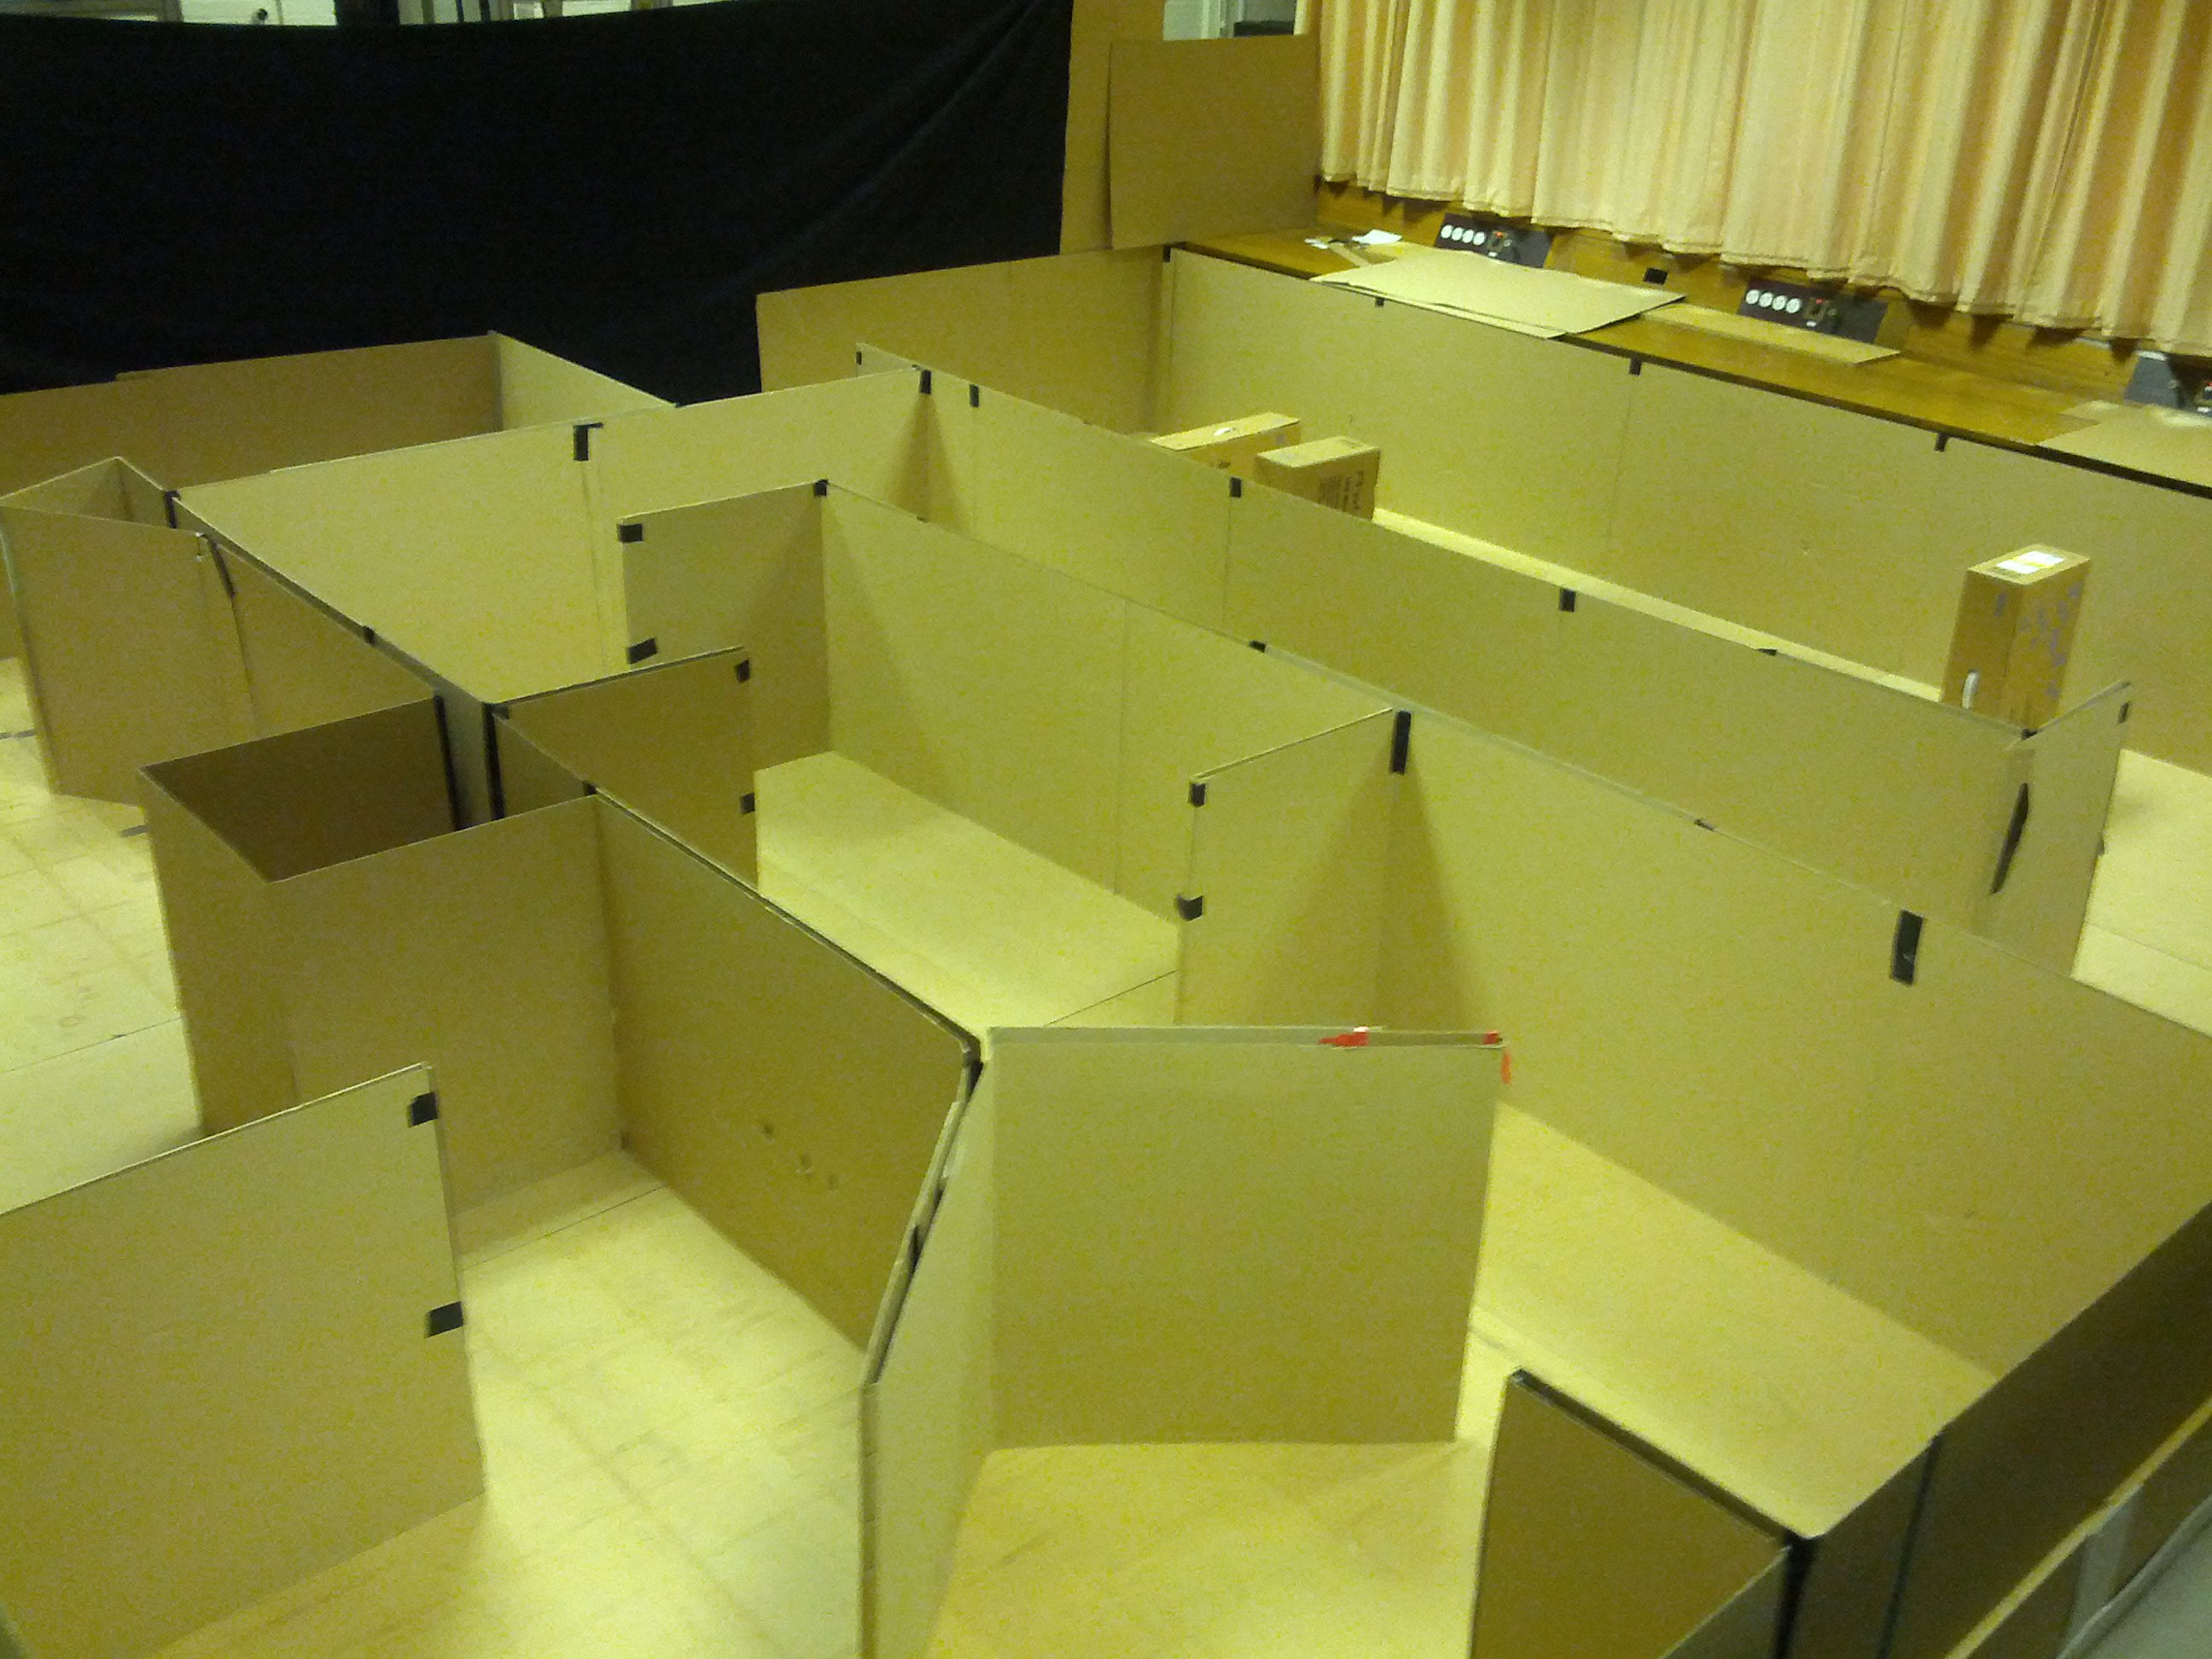
\includegraphics[width=\textwidth]{chapter3_fig/arena_pilot.jpg}
		\label{subfig:arena1_pilot}
	\end{subfigure}
	\hfill
	\begin{subfigure}[b]{0.45\textwidth}
		\centering
		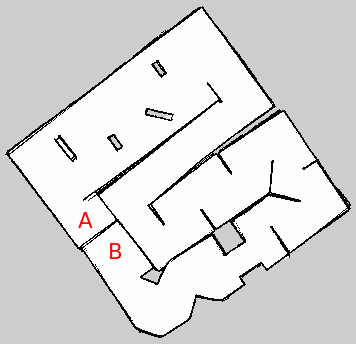
\includegraphics[width=\textwidth]{chapter3_fig/map_pilot.png}
		\label{subfig:map_pilot}
	\end{subfigure}
	\caption{\textbf{Left}: the maze-like arena used in the experiment. \textbf{Right}: a SLAM map of the arena constructed using the robot's onboard laser, and displayed to the human operator on the OCU. Operators are asked to drive from point A to point B and then back again to point A.}
	\label{fig:arena_pilot}
\end{figure}

The primary task was to drive the robot between two points in an obstacle course, as quickly and as accurately as possible (i.e. with the minimum number of collisions). This took place inside an arena of approximately 6.4 x 6 meters (see Fig. \ref{fig:arena_pilot}). It is approximately equivalent to a yellow coded National Institute of Standards and Technology arena \citep{Jacoff2003a}. A secondary task was performed in parallel by the operator and was designed to induce additional workload. In the secondary task a target stimulus (a white dot on a black background) appeared at random intervals on the interface. The operator needed to respond to the presence of the target by pressing a joystick button. The difficulty of the task was controlled by the frequency with which the target appeared on the OCU screen. We considered the secondary task to be the performance degradation factor (load) for the human operator, with two levels, low (i.e target stimulus appeared with low frequency) and high (i.e target stimulus appeared with high frequency).

In terms of robot performance, the degradation factor (load) was the noise in sensor readings with two levels: low and high. High robot load was achieved by means of artificial Gaussian noise added periodically to the laser readings. In the low robot load, no artificial noise was added.

Four conditions were tested: \textbf{Teleoperation with high operator workload}: The operator had to manually drive the robot with a joystick while performing a high difficulty secondary task. Robot load was set to low. \textbf{Teleoperation with low operator workload}: The operator had to manually drive the robot with a joystick while performing a low difficulty secondary task. Robot load was set to low. \textbf{Autonomy with low load}: The operator gave high level commands for the robot to perform autonomously. They were only allowed to switch to teleoperation if it was absolutely necessary for the completion of the trial and only for a dictated period of time. For example if the robot was stuck in a corner, then the operator was required to switch to teleoperation to unstuck. Then, the operator was immediately required to switch back to autonomy. Workload on the secondary task was set to low. \textbf{Autonomy with high load}: The operator gave high level commands for the robot to perform autonomously. He was only allowed to switch mode if it was necessary. Workload on the secondary task was set to low.


\subsection{Participants and experimental design}

The experiment had a between-group design with four groups corresponding to the experimental conditions. In total 28 participants took part, equally distributed among the groups when possible. This distribution was based on their previous experience with driving, video games and operating robots. 

All participants underwent a standardized training procedure. Before the start of the experimental session, participants were required to achieve a minimum performance standard. They had to complete a different obstacle course within a specific time limit, with no collisions, while not missing any secondary task responses. This ensured that all participants started the experiment having attained a minimum standard of proficiency.

Participants were instructed to perform both the primary task and the secondary task as quickly and accurately as possible to the best of their abilities. The map of the arena was not known to the robot or to the operators in advance. Before and during the experiments participants were not permitted to view the arena. Participants had to acquire all information about the arena from the video feed and a progressively acquired laser SLAM map, displayed on the OCU interface.

At the end of the session participants were asked to complete an online NASA Task Load Index (NASA-TLX) \citep{Sharek2011} subjective workload/task difficulty questionnaire.

\subsection{Results}

Analysis was conducted on a series of metrics as elaborated in this section. A two-way analysis of variance (ANOVA) was conducted and Fisher's least significant difference (LSD) for the pairwise group comparisons. Data in some occasions violated ANOVA's assumptions for normality of distribution and homogeneity of variances. However, ANOVA has been proven to be robust in practice when such violations exist. The two factors are the control mode (autonomy and teleoperation) and load (low and high). We use the term ``load'' to describe the amount of degradation induced in the agent who is in control in each condition, i.e. load is the secondary task in teleoperation mode and sensor noise in autonomy mode (artificially added or otherwise). 

% Time to completion
The effect of load on \textit{primary task completion time} was significant, \textit{F(1,22) = 15.525,  $p < .01$}, as was the effect of control mode, \textit{F(1,22) = 40.377, $p < .01$}. The interaction of these two factors was also significant, \textit{F(1,22) = 12.831, $p < .01$} (see Fig. \ref{subfig:totalTime_pilot}) and the statistical power was \textit{$power > .9$}. Pairwise comparison revealed that secondary task high load (high frequency stimulus) and low load (low frequency stimulus) conditions in teleoperation did not have a significant difference. This means that secondary task difficulty does not seem to have an effect on primary task completion time. On the other hand autonomy high load (i.e. added noise to sensor) with a mean of \textit{$M = 1153.8$ $sec$} performed much worse than autonomy low load (i.e. no added noise) (\textit{$M = 517.7$ $sec$}). The difference was significant at \textit{$p <.01$} suggesting that the added sensor noise had a big impact on autonomy performance. Autonomy high load was performed worse than teleoperation high load (\textit{$M = 313.5$ $sec$}) with significance \textit{$p < .01$}. This means that the added noise degrades robot performance more than the high workload secondary task degrades the human operator's performance. A trend can be seen in which teleoperation low load (\textit{$M = 283.2$ $sec$}) performs better than autonomy low load (\textit{$M = 517.7$ $sec$}), but the difference is marginal \textit{$p = .052$}. 

\begin{figure}
	\centering
	\begin{subfigure}[b]{0.49\textwidth}
		\centering
		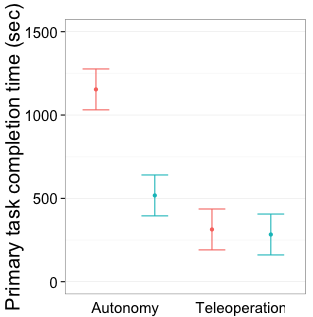
\includegraphics[width=\textwidth]{chapter3_fig/time-cropped_pilot.png}
		\caption{Primary task mean completion time per group.}
		\label{subfig:totalTime_pilot}
	\end{subfigure}
	\hfill
	\begin{subfigure}[b]{0.49\textwidth}
		\centering
		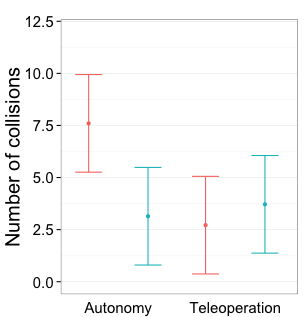
\includegraphics[width=\textwidth]{chapter3_fig/collisions-cropped_pilot.png}
		\caption{Mean collisions among the different groups.}
		\label{subfig:totalCollisions_pilot}
	\end{subfigure}
	\hfill
	\caption{Red is high load, blue is low.}
	\label{fig:time_collisions_pilo}
\end{figure}

%Collisions
Regarding the number of \textit{collisions} (see Fig. \ref{subfig:totalCollisions_pilot}), load, mode and their interaction did not have a significant effect (\textit{$power < .8$}). However collisions seem to be trending towards autonomy high load having a higher number (\textit{$M = 7.6$}) compared to the rest of the groups (teleop-high \textit{$M = 2.7$}, teleoperation low load \textit{$M = 3.7$}, autonomy low load \textit{$M = 3.1$}). This is largely due to the fact that noise distorts the map and thus the robot's ability to autonomously navigate degrades.  

% Primary score
\textit{Primary task score}, compensates for the individual differences in speed-accuracy trade-off (i.e. time vs collisions). It was calculated by adding \textit{$10 sec$} of penalty to the task completion time for every collision. With \textit{$power > .9$} the effects of load (\textit{F(1,22) = 13.003,  $p < .05$}), mode (\textit{F(1,22) = 33.067, $p < .01$}) and interaction (\textit{F(1,22) = 11.541, $p < .05$}) on primary task score were significant (see Fig. \ref{subfig:primary_score_pilot}). The condition that had significant difference from the rest was autonomy high load (\textit{$M = 1229.8$, $p < .01$}).
 
 \begin{figure}
 	\centering
 	\begin{subfigure}[b]{0.46\textwidth}
 		\centering
 		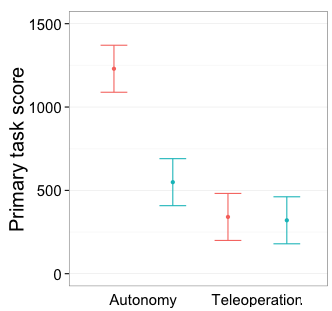
\includegraphics[width=\textwidth]{chapter3_fig/primary_score_cropped_pilot.png}
 		\caption{Primary task score per group.}
 		\label{subfig:primary_score_pilot}
 	\end{subfigure}
 	\hfill
 	\begin{subfigure}[b]{0.52\textwidth}
 		\centering
 		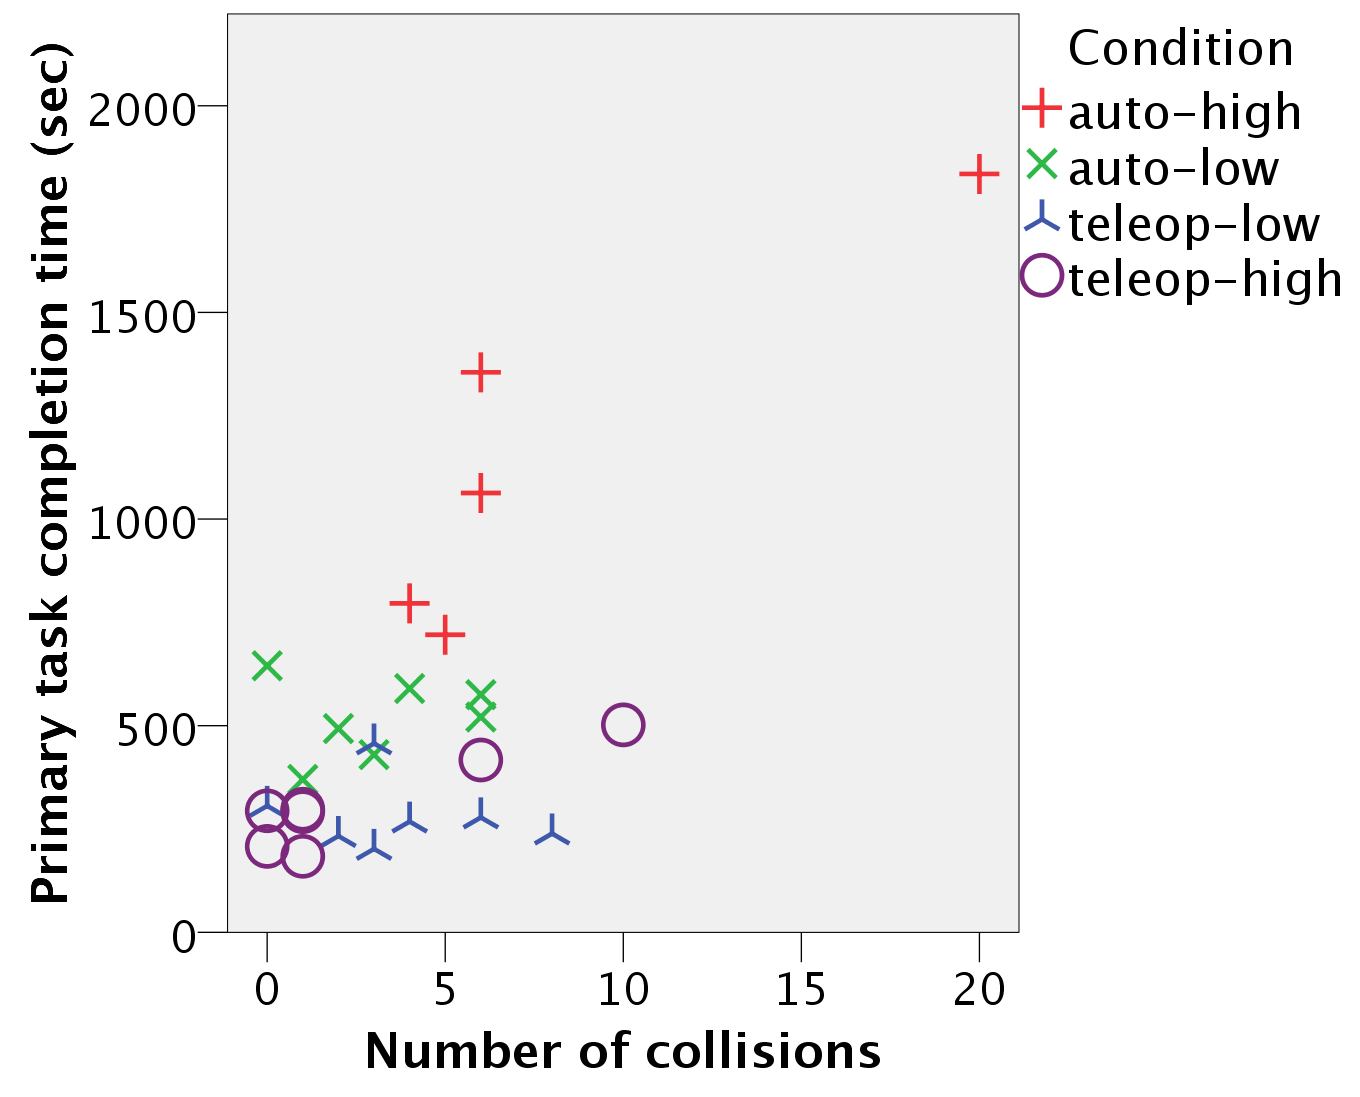
\includegraphics[width=\textwidth]{chapter3_fig/speed-acc_pilot.png}
 		\caption{Individual participant primary task performance.}
 		\label{subfig:speed_acc_pilot}
 	\end{subfigure}
 	\hfill
 	\caption{In \ref{subfig:primary_score_pilot} red is high load, blue is low.}
 	\label{fig:score-speed-acc_pilot}
 \end{figure}
 
%SPEED-ACC
\textit{Individual participant performance} on the two primary task metrics (see Fig. \ref{subfig:speed_acc_pilot}), shows no obvious groups. This is in terms of operator strategies favoring speed or accuracy over the other. It seems that there are some participants that perform generally worse and participants that perform generally better.

% RT
In terms of secondary task performance, i.e. \textit{reaction time} (see Fig. \ref{subfig:totalRT_pilot}), ANOVA (\textit{$power < .8$}) showed that the main effects for load and mode are not significant. The interaction however is significant with \textit{F(1,22) = .4.638, $p < .05$}. Pairwise comparisons between the groups showed that the difference between teleoperation high load (\textit{$M = 0.588$ $sec$}) and teleoperation low load (\textit{$M = 0.717$ $sec$}) is marginally significant \textit{$p =.05$} with the rest of the comparisons not being significant.

 \begin{figure}
 	\centering
 	\begin{subfigure}[b]{0.4\textwidth}
 		\centering
 		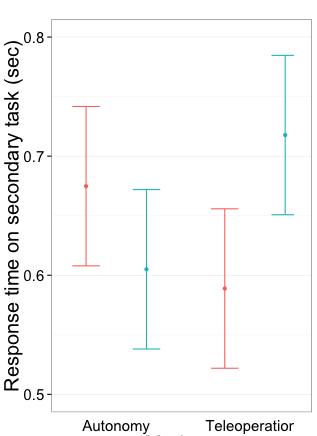
\includegraphics[width=\textwidth]{chapter3_fig/RTs-cropped_pilot.png}
 		\caption{Mean reaction time for each group.}
 		\label{subfig:totalRT_pilot}
 	\end{subfigure}
 	\hfill
 	\begin{subfigure}[b]{0.4\textwidth}
 		\centering
 		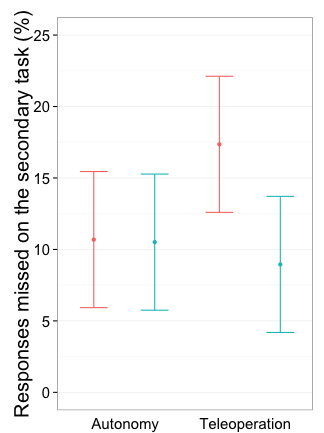
\includegraphics[width=\textwidth]{chapter3_fig/misses-cropped_pilot.png}
 		\caption{Percentage of missed responses for each group.}
 		\label{subfig:totalMissedRT_pilot}
 	\end{subfigure}
 	\hfill
 	\caption{Secondary task performance. Red is high load, blue is low.}
 	\label{fig:rt_pilot}
 \end{figure}

%Missed RT
The \textit{rate of missed responses} (i.e number of missed responses over the number of targets presented on the display) in the secondary task was also measured. ANOVA with \textit{$power < .8$} showed that differences were not significant. In Fig. \ref{subfig:totalMissedRT_pilot} the rate of missed responses is presented for reference. Playback of the recorded trials and informal discussion with the participants provided useful insight regarding missed responses. In most cases for teleoperation, they occurred during a difficult navigation maneuver or when the operator was trying to acquire SA or both. During autonomy mode, greater rates of missed responses occurred during periods when a) AI performance dropped, e.g. the robot became stuck or lost localization; b) when a human operator was trying to infer what the robot was doing; c) when the operator was giving a command.

% NASA-TLX
\textit{NASA-TLX scores} suggest that participants found all of the different conditions equally difficult, as ANOVA (\textit{$power < .8$}) showed no significant difference. This means that the degraded/high load trials were not difficult enough to be consciously perceived as such  by the participants.

It should be noted that the data from two participants in the conditions autonomy high load and autonomy low load were removed from this analysis as the trials were not completed.

\subsection{Discussion}
It proved unexpectedly difficult to extract a clear analysis or definitive interpretation of the results. This is mainly due to the small number of participants per group and the high variance in performance between trials. There were a number of confounding factors that could have affected the latter and need careful consideration as discussed here and in Section \ref{chap3:guidelines}.

Firstly the degradation factors for the two agents did not cause an equivalent effect, as assumed during the experimental design. Results show that the sensor noise degrading effect on the robot was higher than the effect of the high workload secondary task on the human. Thus, in the later experiments, we changed the secondary task to make it more difficult, i.e. more intrusive; demanding more cognitive resources. This allowed the new secondary task to match the autonomy degradation factor in order for these to become meaningfully comparable. In general, the autonomy high load condition performs the worst in terms of primary task performance.

Counter-intuitively, participants were faster to respond to stimulus in the teleoperation high load condition than in the teleoperation low load condition. This could be due to the fact that participants may feel more engaged and alerted when they have to respond to a more frequent stimulus.

\section{Suggestions for future experiments}
\label{chap3:guidelines}
This section presents observations and lessons learned that lead to a more systematic experimental design in the context of variable autonomy mobile robotics research. It is based on the findings presented in this chapter and is focused on how to control for confounding factors and minimize result variance while maintaining all those elements that allow for meaningful scientific investigation.

One of the primary considerations is the difficulty and the nature of the tasks. Regarding the difficulty of the navigation task, most of the arena should be simple for the robot to navigate autonomously. However, some parts should be impossible for the robot without human intervention. This will yield more significant results by avoiding variance in performance of the autonomy between trials, caused by unpredictable situations. For example a robot that sometimes is able to pass through a narrow passage, while other times is stuck in the same passage. Also the arena map should be fully known in advance, and presented to each participant in the same way with the same accuracy. This will minimize the variance in performance caused by different human operator strategies for exploring an unknown map. In the context of our research, tasks have to be designed such that they genuinely necessitate the use of both teleoperation and autonomy in order to be better or successfully completed. In this way the collaborative potential (i.e. between the human and the AI) that variable autonomy offers can be investigated. This is congruent with real world deployment of robots in which the strengths of both agents are needed.

The experimental protocol plays a key role in controlling for individual differences between participants. For example a within-subjects design is more likely to control for individual differences. This is preferable over avoidance of possible training effects, given the variance of the results presented in this chapter. Moreover it is a more efficient use of resources. Also of particular importance are participants' experience and skill level. Extensive participant training makes experiments time consuming. However, this ensures participants share a minimum skill level, trust the autonomous system, and fully understand its capabilities and limitations. This can improve the HRI, and minimize variability between different participants. An example of a problematic interaction is the tendency that many human operators exhibit of overriding correct autonomous actions. This is because they mistakenly believe these actions are not contributing towards the goal \citep{Marble2004}.

Choosing appropriate metrics and measurement techniques is not trivial and requires careful consideration. As discussed in Section \ref{section:chapter3-pilot}, SA affects performance but it can be complex to measure, e.g. no real-time measurement; highly intrusive techniques. Measuring SA implicitly through task performance can be better suited than other methods in the current context. Similar to SA, operator workload is difficult to measure in real time without using physiological techniques, such as EEG (see Section \ref{chapter2:workload}). Also, counter-intuitively, high workload does not necessarily cause task performance to degrade. Predictions on performance degradation during task execution, based on the measured workload level, can only be made if a correlation between them is found.

Lastly, the experiments need to explicitly contribute towards MI variable autonomy. This has to be reflected on the experimental design. A MI system needs to \emph{jointly} consider both degraded task performance and the context and timing of the performance measurements. For example, if a human is attempting a very difficult maneuver or operation, this may produce degraded performance using a particular metric (e.g. slow progress towards a navigational goal). However, giving control to the robot in this context could be problematic, e.g. causing a collision or the robot to get stuck. Despite the complexity, measuring degraded performance jointly with context, might be simplified by designing experiments that use "idle time" as an additional performance metric. This can be defined as the time passed without any progress towards achieving a goal. In teleoperation, idle time includes times when an operator is neglecting the robot. In autonomy it includes time which passes without the robot controller actively achieving something, e.g. the robot sits stuck in a corner or stuck in front of an obstacle. This is similar to the ``neglect time'' metric proposed by Goodrich and Olsen \citep{Goodrich2003}. However, it is simpler and more easily applied to multiple conditions and tasks.


\section{Conclusion and impact}
\label{chap3:conclusion}

Our initial experiment aimed to explore the performance of human operators and the robot under different conditions and to address the lack of a rigorous experimental framework. It provided some useful insights and interesting results that informed the design of the experiments presented in the later chapters. 

Firstly, the simple reaction time secondary task proved inappropriate, mainly because of its unclear impact on performance. However, the system's performance degraded significantly with noise that distorted the robot's model of the world. In order to objectively infer when a LOA switch is needed, the different experimental conditions should be able to degrade performance in a consistent and measurable way. A variety of different secondary tasks such as arithmetic tasks; SA tasks (e.g. the operator being asked to provide information to the experimenter during trials); and tasks that can be cooperatively performed by both agents; can be used towards this direction.

Secondly, designing and conducting principled experiments, which yield statistically meaningful insights in this context, has proved to be a challenging task. Mainly this is due to the intrinsic complexity of combining human factors with a robotic system. A multidisciplinary approach is required, taking into account robotics, human factors, psychology and HRI. There are a plethora of confounding factors that can distort results and make meaningful inference intractable. An important aim of this chapter is to communicate to the research community the lessons learned, and suggestions for a systematic experimental framework, that we have arrived at through carrying out our pilot-study experiment.

Lastly, constraining the physical conditions and the experimental design in appropriate ways might help in reducing complexity. However, such results might not be practically meaningful or useful if the environment is excessively sterilized or artificially constrained. With the suggestions presented in this chapter, we have moved towards a cleaner and more principled experimental design, rather than a restricted or sterilized one, that can provide data that is meaningful to real-world robotic systems, but is also collected scientifically under controlled laboratory conditions.

\chapter{EXPERIMENTAL ANALYSIS OF HUMAN-INITIATIVE VARIABLE AUTONOMY}\label{chapter4:HI}
This experiment develops from our previous work described in Chapter \ref{chapter3:towards} and it is based on our published papers in IEEE/RSJ International Conference on Intelligent Robots and Systems (IROS) \citep{Chiou2016} (finalist for best paper award on cognitive robotics) and in AAAI 2016 fall symposium series \citep{Chiou2016_AAAI}. Based on the lessons learned in our previous experiment, a rigorous experimental paradigm was informed that allows the principled study of variable autonomy. More specifically, the framework was improved compared to the one in Chapter \ref{chapter3:towards} by: a) minimizing confounding factors, e.g. by using extensive participant training and a within-subject design; b) introducing a meaningful (i.e. enough difficulty to degrade primary task performance) secondary task for human operators; and c) introducing a variable autonomy controller.  This multidisciplinary framework is drawing on methodologies from the fields of psychology and human factors, as well as engineering and computer science. The absence of such a framework in existing literature was highlighted in previous sections (e.g. in \ref{section:framework_lit}). Thus, we consider the framework used here to be a significant contribution.

In the experiment described here, we compare the performance of three different systems: 1) pure joystick teleoperation of a mobile robot; 2) a semi-autonomous control mode (which we refer to hereafter as the ``autonomy'' LOA) in which a human operator specifies navigation goals to which the robot navigates autonomously; 3) a Human-Initiative (HI) variable autonomy system, in which the human operator can dynamically switch between the teleoperation and autonomy modes using a button press. During experiments, human test subjects are tasked with navigating a differential drive vehicle around a maze-like test arena, with SA provided solely by a monitor-displayed control interface. At various points during the experiments, the robot's performance is degraded by artificially introducing controlled amounts of noise to sensor readings, and the human operator's performance is degraded by forcing them to perform a cognitively complex secondary task.  Our hypothesis is that the HI system will enable superior navigation performance compared to either teleoperation or autonomy alone, especially in scenarios where the performance of both the human and the robot may at times become degraded. We evaluated our hypothesis through carefully controlled and repeatable experiments using a significant number of participants.

Issues of variable autonomy robotics comprise two different but highly coupled elements: robotics engineering and computation; and Human-Robot Interaction (HRI). The first element addresses autonomous control capabilities, and how are they integrated into a robot system. The second element refers to all aspects of the human operator interacting and cooperating with the variable autonomy robot as part of a team. It includes factors such as trust in autonomous control technologies, the operator's personal preferences, and the operator's use of the robot's autonomous abilities. Here we provide analysis on both of these elements.

First, an analysis is provided focused on overall system performance with respect to the primary task of robot navigation through a complex environment. The results present (for the first time - to the best of our knowledge, see Section \ref{section:HI-background}) scientific evidence proving that variable autonomy can outperform both pure teleoperation and pure autonomy in various circumstances. Then, an analysis focused on the HRI aspects of the human operator interacting with and exploiting the HI controller is provided. More specifically we report on: the human operators' preferred LOA; the amount of time spent in each LOA; the frequency of human-initiated LOA switches; human perceptions of the difficultly of using HI variable autonomy systems. We also investigate the correlation between these variables; their correlation with performance in the primary task (navigation of the robot); and their correlation with performance in a secondary task. To the best of our knowledge, as described in Section \ref{section:HRI_LOA_switch}, our work is the first on mobile robots that reports a statistical analysis of the ways in which human operators interact with a robotic system in which LOA modes can be dynamically switched.

Lastly, the experiment reported here focuses on the ability and authority of a human operator to switch LOA on the fly, based on their own judgment. We define (see Section \ref{section:HI-background}) this form of variable autonomy as Human-Initiative (HI), in contrast to Mixed-Initiative (MI) systems (see Section \ref{section:MI-taxonomy}) in which both the AI and the operator have the authority to initiate LOA changes. However, results and insights gathered during this experiment have additionally been used to inform the design of a Mixed-Initiative (MI) system as reported in the next chapter (see Section \ref{chapter5:general_expert_MI}).

\section{Apparatus and robotic software}
Our robot and environment were simulated in the Modular Open Robots Simulation Engine (MORSE) \citep{Echeverria2011}, which is a high fidelity simulator (i.e. realistic graphics, physics and robot model). The robot used was a Pioneer-3DX mobile robot equipped with a laser range finder sensor and a RGB camera. The robot is controlled by the Operator Control Unit (OCU), composed of a laptop, a joystick, a mouse and a screen showing the control interface (see Fig. \ref{fig:interface_exp2}).

In our previous experiment, in \citep{Chiou2015} and Chapter \ref{chapter3:towards}, we built a large maze-like test arena (see Fig. \ref{subfig:arena_real_exp2} and Fig. \ref{subfig:map_real_exp2}), and carried out human-subject tests using a real Pioneer-3DX robot fitted with camera, laser scanner and WiFi communication to the remote Operator Control Unit. While demonstrating new methods on real robots is important, we observed that this can introduce difficult confounding factors, which can detract from the repeatability of experiments and the validity of collected data. Major confounding factors include individual differences in personality traits; experience on operating robots or playing video games; map exploration strategies; WiFi communication delays (e.g. in the commands or in the video feedback). Minor confounding factors include tests at different times of day or different weather, mean that daylight levels inside the lab change, affecting the video images observed by each test-subject. Different amounts of battery charge can cause top speed of the robot to vary slightly between different test-subjects. These and other factors led us to design the experiments reported in this paper using a high fidelity simulated robot and test-arena. As can be seen in Fig. \ref{fig:arenas_exp2} and Fig. \ref{fig:maps_exp2}, and comparing the real and simulated video feeds (Fig. \ref{fig:interface_exp2} and Fig. \ref{fig:various_real_exp2}), the simulation environment creates very similar situations and stimuli for the human operators as experienced when driving the real robot, but with a much higher degree of repeatability.

\begin{figure}
	\centering
	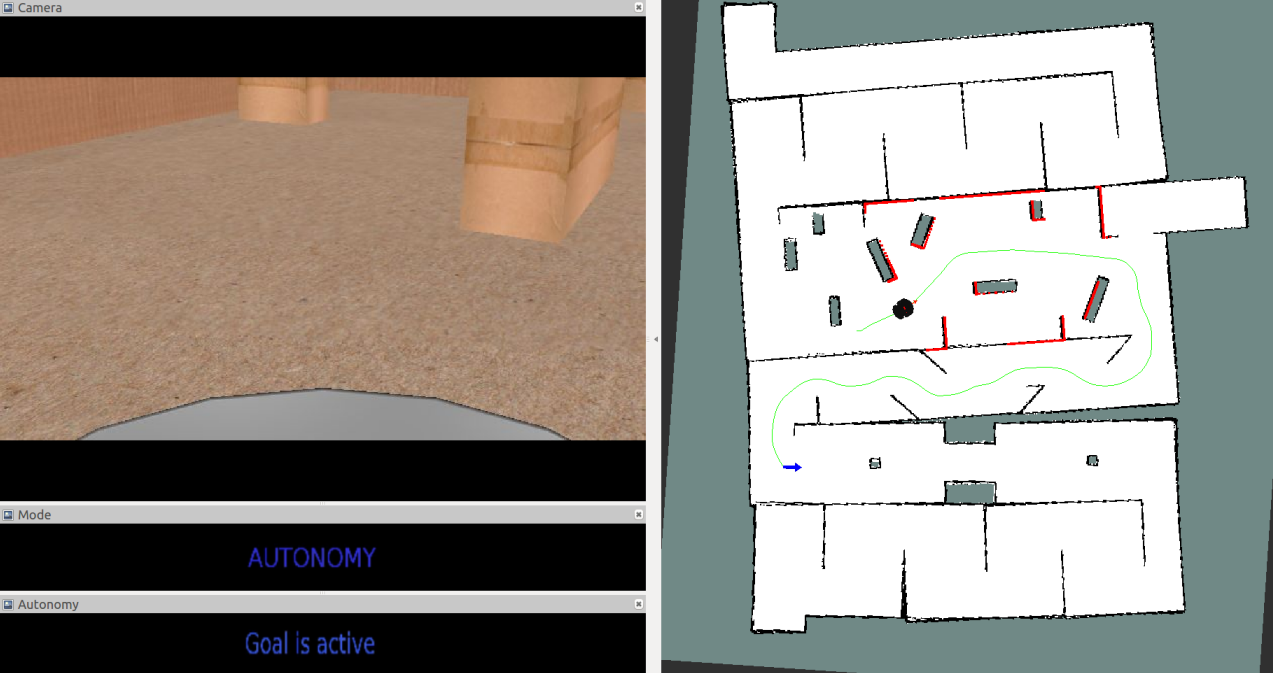
\includegraphics[width=0.8\columnwidth]{chapter4_fig/interface.png}
	\caption{The control interface as presented to the operator. \textbf{Left}: video feed from the camera, the control mode in use and the status of the robot. \textbf{Right}: The map showing the position of the robot, the current goal (blue arrow), the AI planned path (green line), the obstacles' laser reflections (red) and the walls (black).} 
	\label{fig:interface_exp2}
\end{figure}

Our system offers two LOAs. \textbf{Teleoperation:} the human operator drives the robot with the joystick, while gaining SA via a video feed from the robot's onboard RGB camera. Additionally a laser generated 2D map is displayed on the OCU. \textbf{Autonomy:} the operator clicks on a desired location on the 2D map, then the robot autonomously plans and executes a trajectory to that location, automatically avoiding obstacles. The system is a \textbf{Human-Initiative (HI)} system as the operator can switch between these LOAs at any time by pressing a joystick button. The software used was developed in Robot Operating System (ROS) and is described in more detail in Section \ref{chapter3:system}.

\section{Experimental design and procedure}

This experiment investigates to what extent circumstances in which the robot is under-performing can be overcome or improved by switching control between the AI and the human operator. Such circumstances can be captured by idle time, which is the time passed without any progress towards achieving a goal (see \citep{Chiou2015} or Section \ref{chap3:guidelines}). For example a robot being neglected by its operator when in teleoperation mode, or stuck due to a navigation failure in autonomy mode. Similar situations are quite common in real world robotics deployments \citep{Murphy2004}. For example, consider the case in which a robot operator must interrupt their control of the robot, to provide information to the SAR team leader or EOD team commander. Our hypothesis is that in such circumstances, trading control to another agent will improve the overall task performance of the system. 

\begin{figure}
		\centering
		\begin{subfigure}[b]{0.48\textwidth}
			\centering
			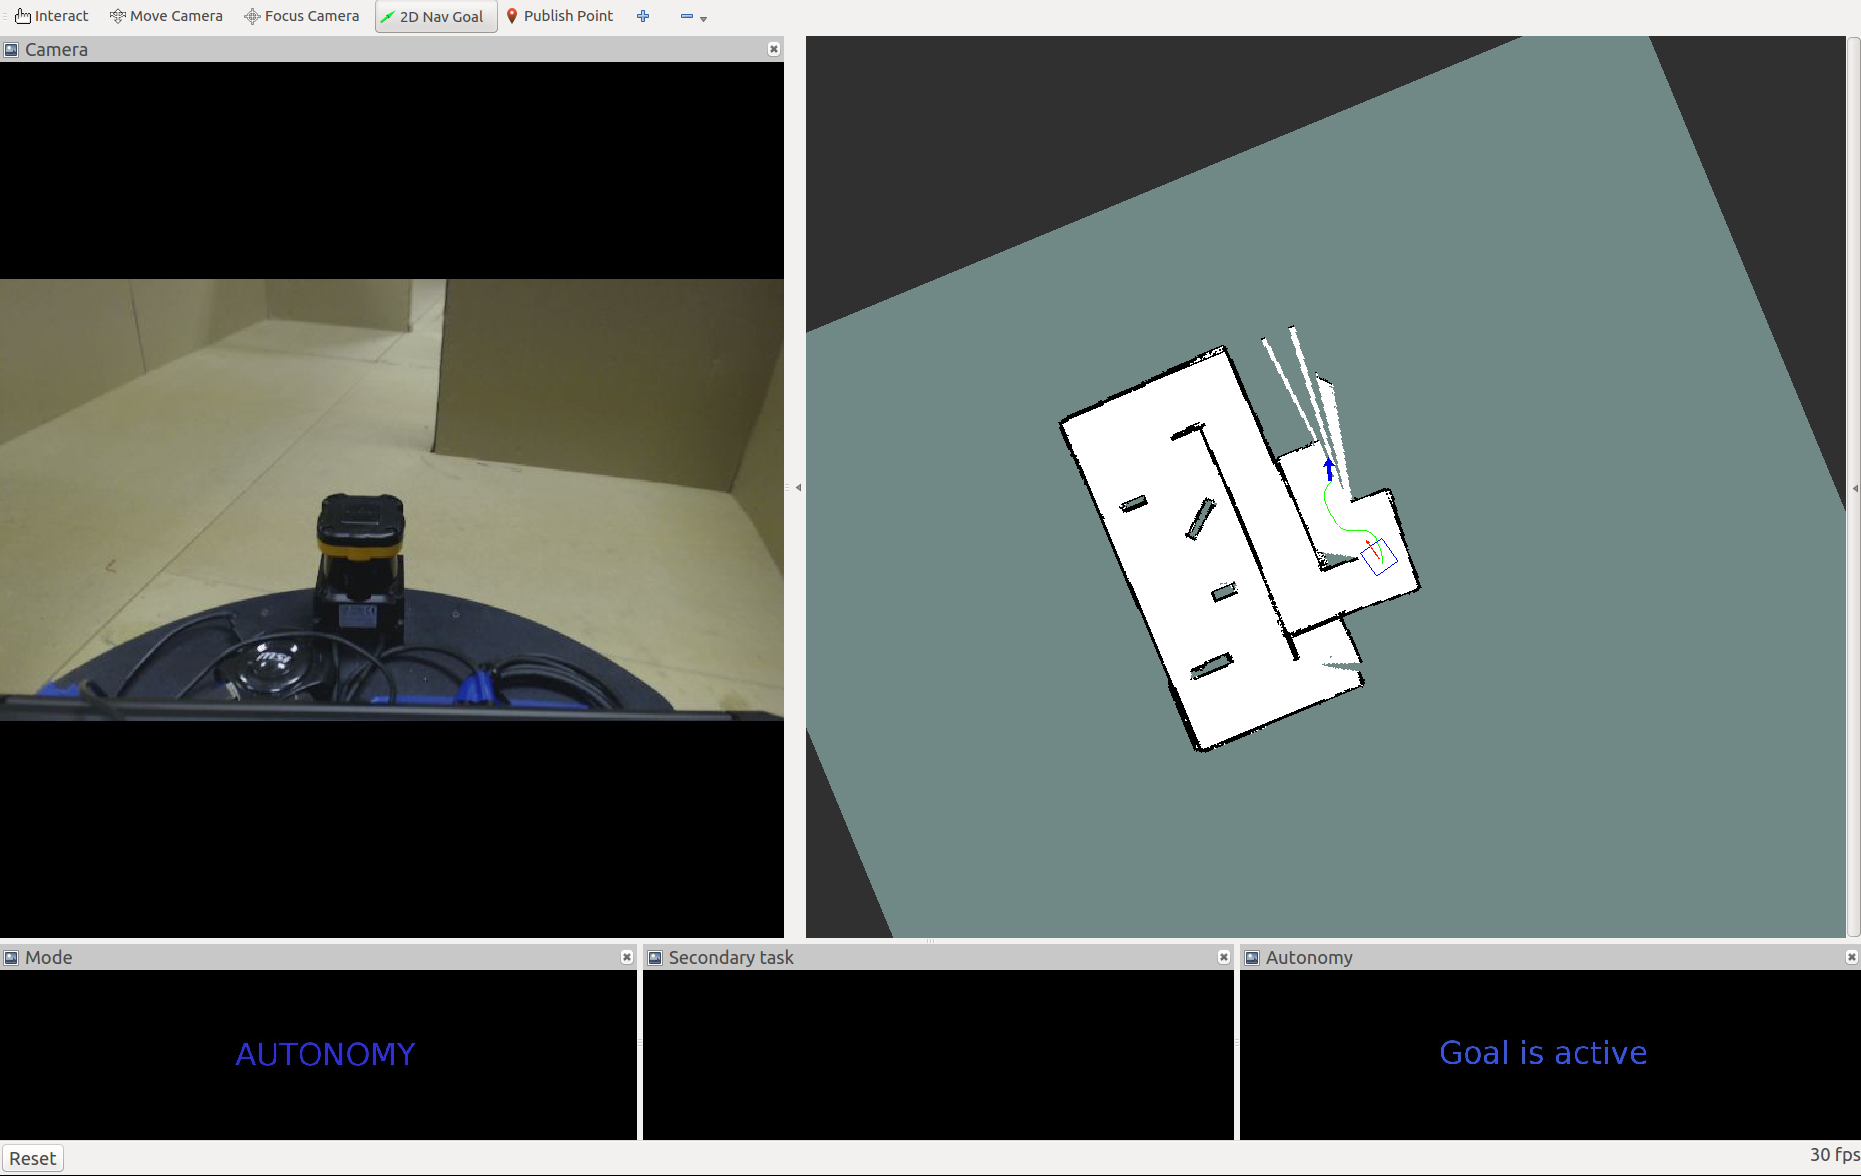
\includegraphics[width=\textwidth]{chapter4_fig/interface_real.png}
			\caption{}
			\label{subfig:interface_real_exp2}
		\end{subfigure}
		\hfill
		\begin{subfigure}[b]{0.49\textwidth}
			\centering
			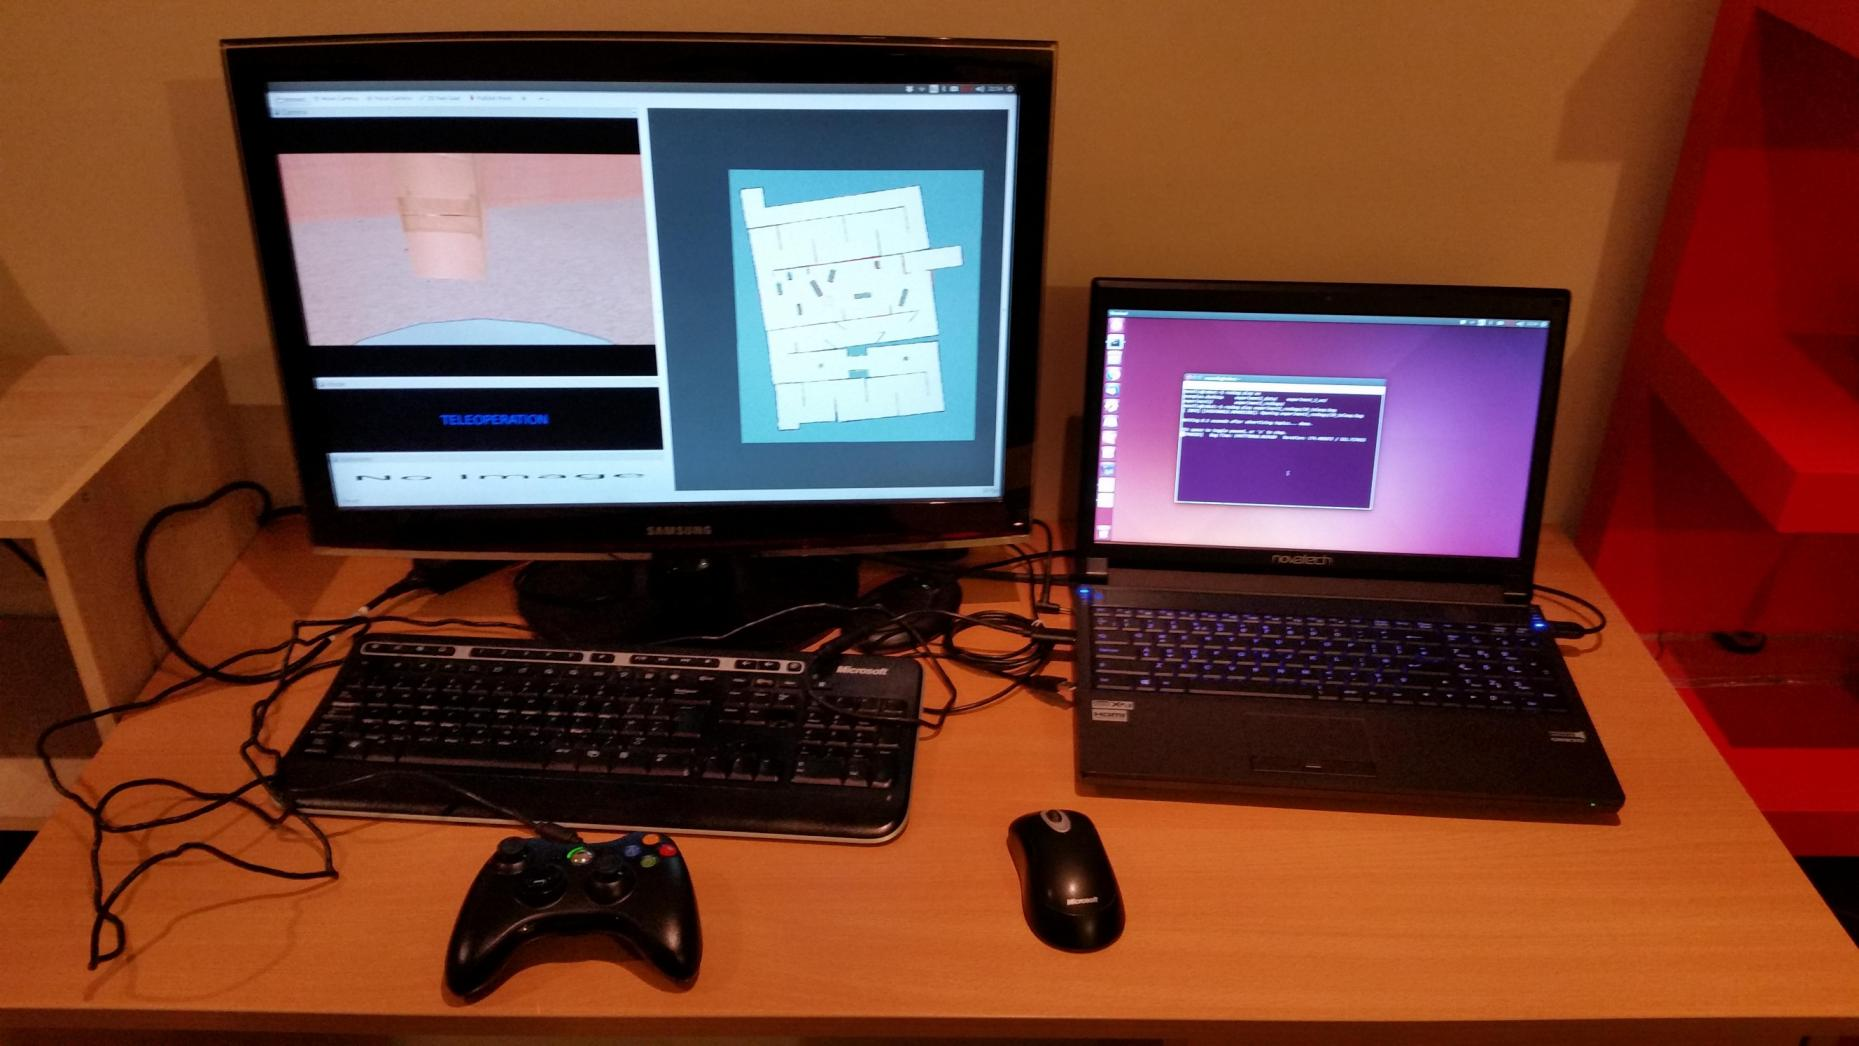
\includegraphics[width=\textwidth]{chapter4_fig/OCU.jpg}
			\caption{}
			\label{subfig:OCU_exp2}
		\end{subfigure}
		\hfill
		\caption{ \textbf{\ref{subfig:interface_real_exp2}:} the control interface as presented to the operator in our previous real world experiment. \textbf{\ref{subfig:OCU_exp2}:} the Operator Control Unit (OCU), composed of a laptop, a joystick, a mouse and a screen showing the control interface. The same OCU was used in both experiments.}
		\label{fig:various_real_exp2}
	\end{figure}

\subsection{Experimental setup - operator control unit and robot test arena}
	
In the work described in this paper, we used an identical OCU (see Fig. \ref{subfig:OCU_exp2}) as that used in our previous experiments with a real robot \citep{Chiou2015}. A simulated maze was designed with dimensions of  $11 \times 13.5$ meters (see Fig. \ref{subfig:arena_exp2} and Fig. \ref{subfig:map_exp2}). It approximates a yellow coded National Institute of Standards and Technology arena \citep{Jacoff2003a}. As can be seen in Fig. \ref{subfig:map_real_exp2} and Fig. \ref{subfig:interface_real_exp2}, the data presented to the human operator via the OCU is almost identical to that experienced by human test subjects operating the real robot in a real arena in our prior work.
	
\begin{figure}
	\centering
	\begin{subfigure}[b]{0.45\textwidth}
		\centering
		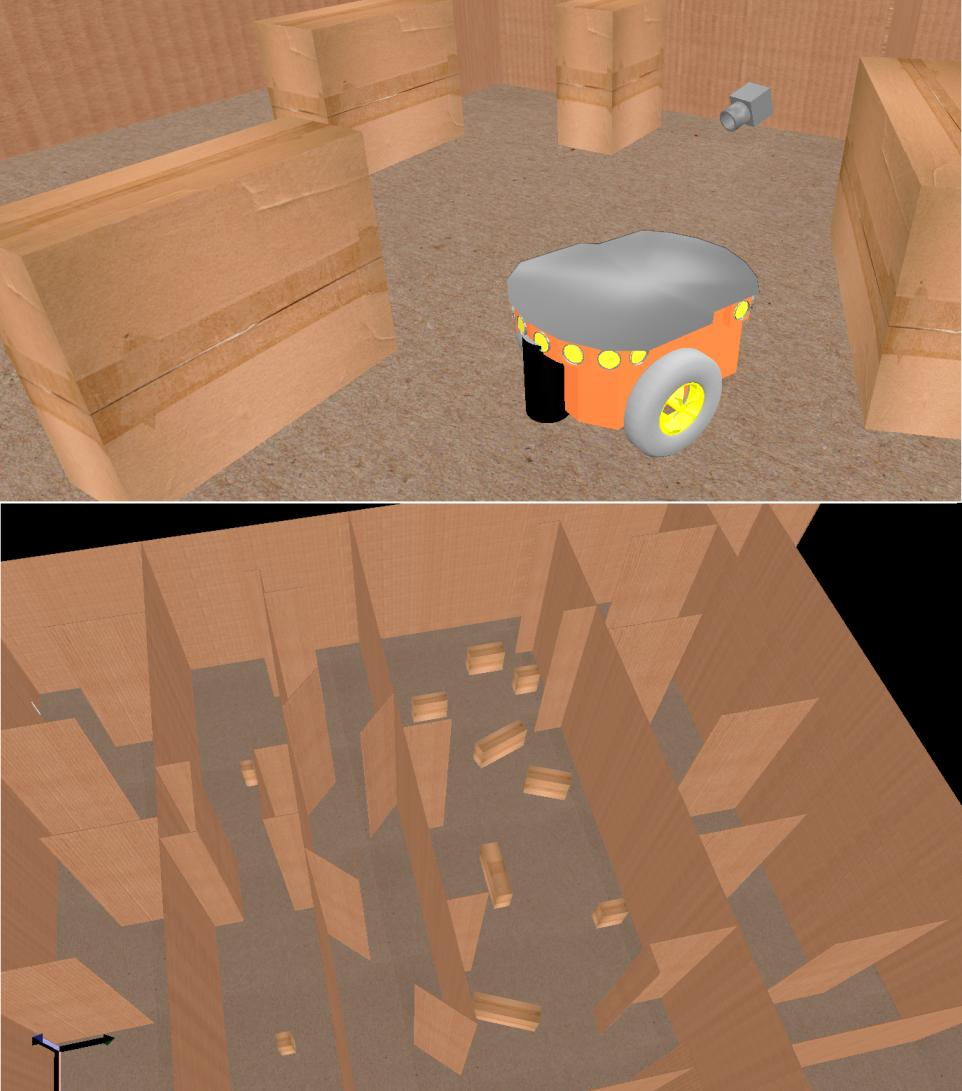
\includegraphics[width=\textwidth]{chapter4_fig/sim2.jpeg}
		\caption{The simulated arena and the robot model used in the experiment.}
		\label{subfig:arena_exp2}
	\end{subfigure}
	\hfill
	\begin{subfigure}[b]{0.35\textwidth}
		\centering
		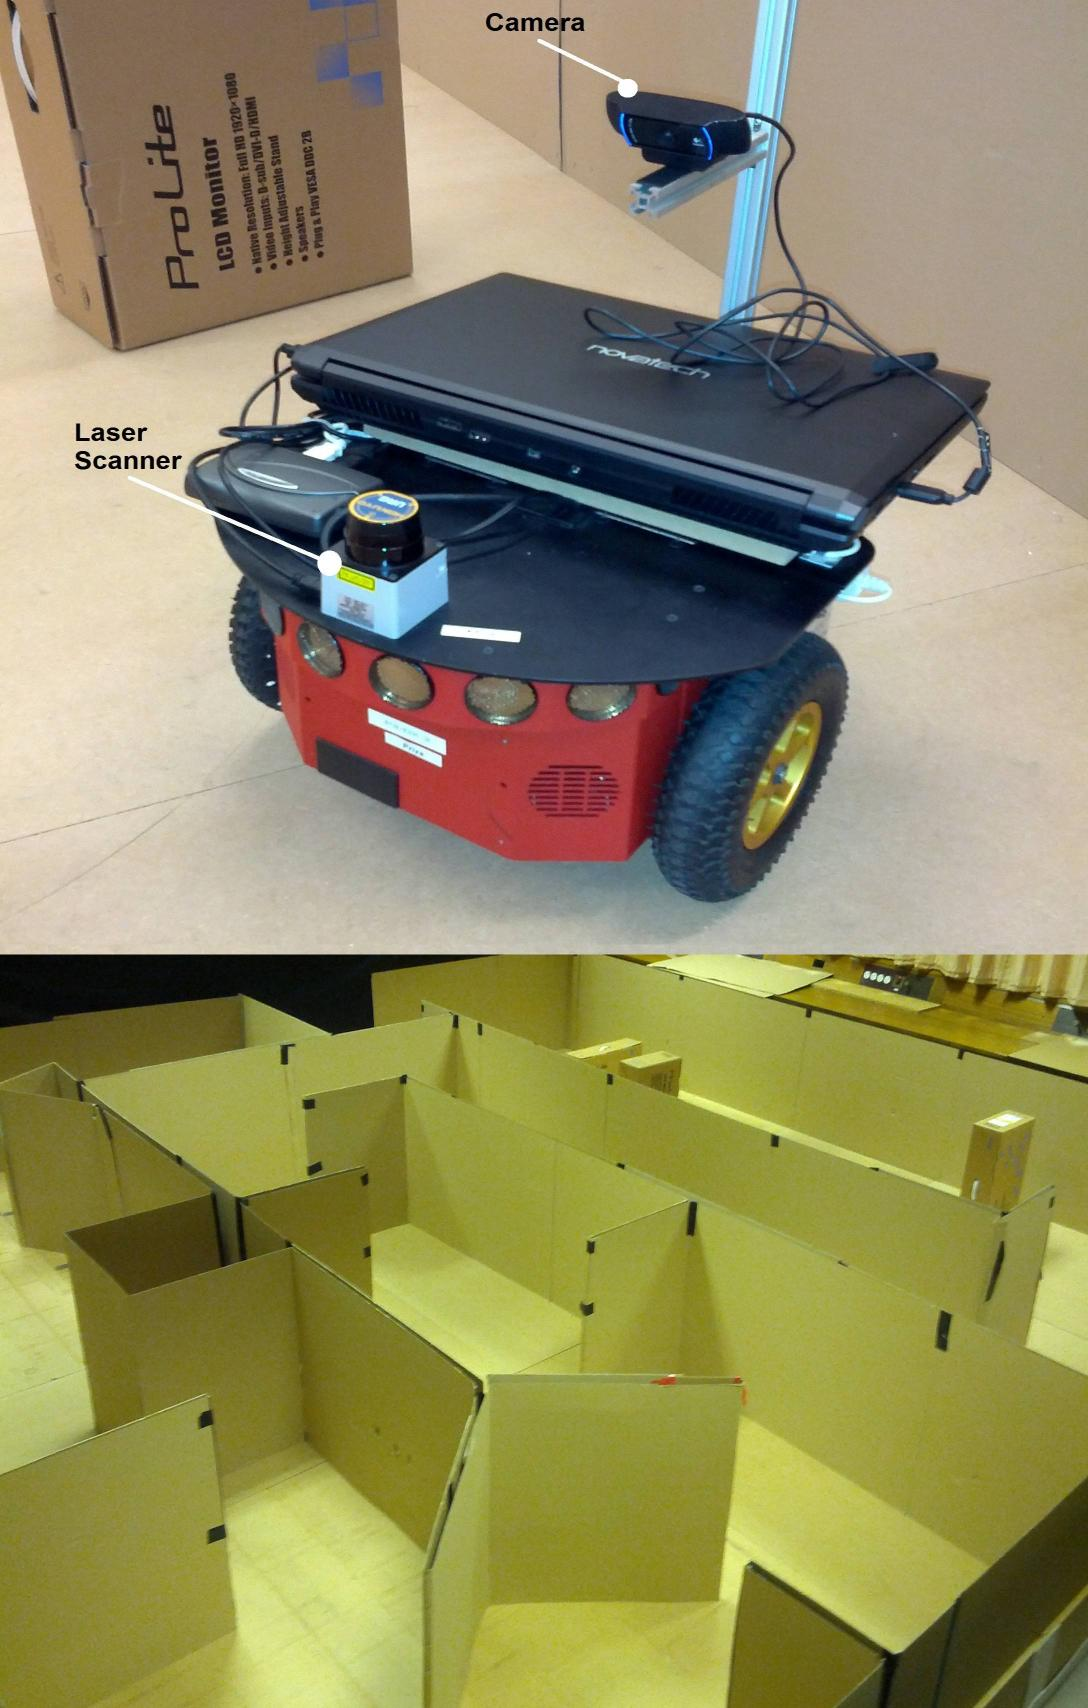
\includegraphics[width=\textwidth]{chapter4_fig/arena_real.jpeg}
		\caption{The real arena and robot used in our previous experiment.}
		\label{subfig:arena_real_exp2}
	\end{subfigure}
	\hfill
	\caption{Note that the simulation recreates the real environment with a good degree of fidelity.}
	\label{fig:arenas_exp2}
\end{figure}

\begin{figure}
	\centering
	\begin{subfigure}[b]{0.41\textwidth}
		\centering
		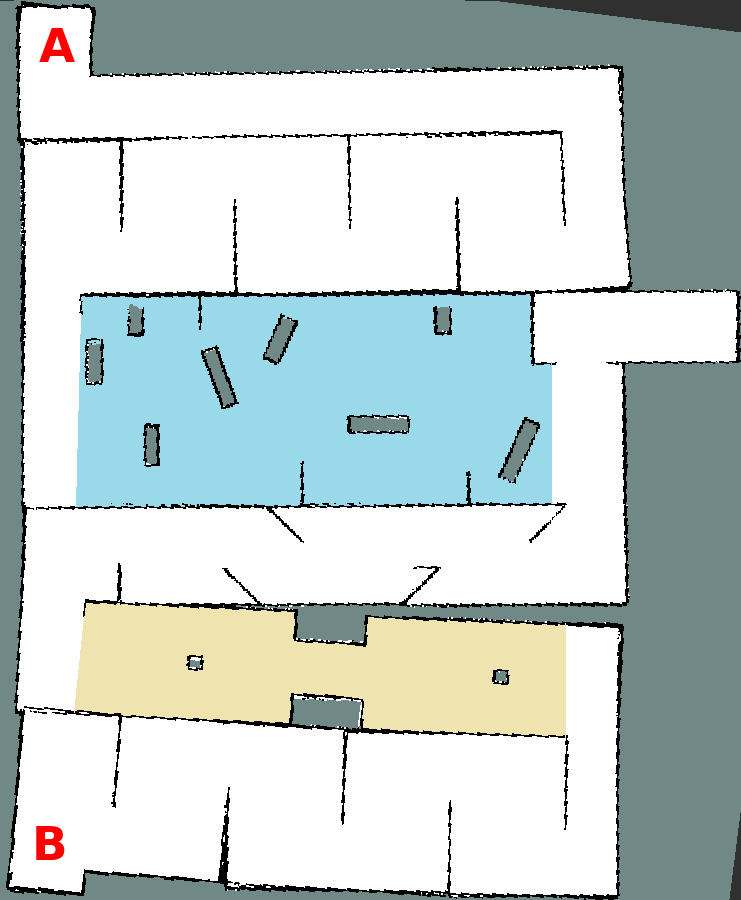
\includegraphics[width=\textwidth]{chapter4_fig/map.png}
		\caption{}
		\label{subfig:map_exp2}
	\end{subfigure}
	\hfill
	\begin{subfigure}[b]{0.45\textwidth}
		\centering
		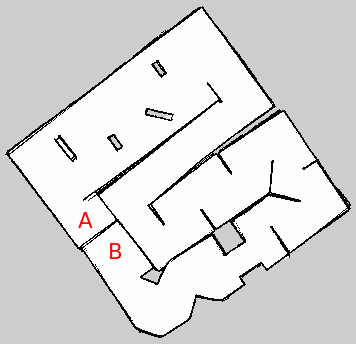
\includegraphics[width=\textwidth]{chapter4_fig/map_real.png}
		\caption{}
		\label{subfig:map_real_exp2}
	\end{subfigure}
	\hfill
	\caption{\textbf{\ref{subfig:map_exp2}:} laser-derived SLAM map created in the simulation environment. Primary task was to drive from point A to B and back again to A. The yellow shaded region is where artificial sensor noise was introduced. The blue shaded region is where the secondary task was presented to the operator. \textbf{\ref{subfig:map_real_exp2}:} laser-derived SLAM map generated by real robot in our previous experiment. Note the similarities between the real and simulated data.}
		\label{fig:maps_exp2}
	\end{figure}
	
\subsection{Primary and secondary tasks, and experimental test modalities}
Each human test subject was given the primary task of navigating from point A in Fig.~\ref{subfig:map_exp2} (the beginning of the arena) to point B (the end of the arena) and back to point A. The path was restricted and one way, i.e. no alternative paths existed in order to prevent different operator's from using different paths and thus avoiding a potential confounding factor.
	
Two different kinds of performance degrading factors were introduced, one for each agent: artificially generated sensor noise was used to degrade the performance of autonomous navigation; and a cognitively intensive secondary task was used to degrade the performance of the human test subject. In each experimental trial, each of these performance degrading situations occurred twice, once on the way from point A to point B, and a second time on the way from point B back to point A. The two different kinds of degradations occurred separately from each other, as shown in Fig. \ref{subfig:map_exp2}.
	
More specifically, autonomous navigation was degraded by adding Gaussian noise to the laser scanner range measurements, thereby degrading the robot's localization and obstacle avoidance abilities. This was achieved by adding to each individual laser measurement Gaussian noise with zero mean and $\sigma$ proportional to the measured distance, i.e. the longer the distance of the measurement the bigger the added noise. For every experimental trial this additional noise was instantiated when the robot entered a pre-defined area of the arena, and was deactivated when the robot exited that area.
	
To degrade the performance of the human operator, their cognitive workload was increased via a secondary task of mentally rotating 3D objects. Whenever the robot entered a predefined area in the arena, the test subject was presented with a series of 10 cards, each showing images of two 3D objects (see Fig. \ref{fig:rotation_task_exp2}). In half of the cards, the objects were identical but rotated by 150 degrees. In the other half the objects were mirror image objects with opposite chiralities. The test subject was required to verbally state whether or not the two objects were identical (i.e. yes or no). This set of 3D objects was previously validated for mental rotation tasks in \citep{Ganis2015}.
	
	\begin{figure}
		\centering
		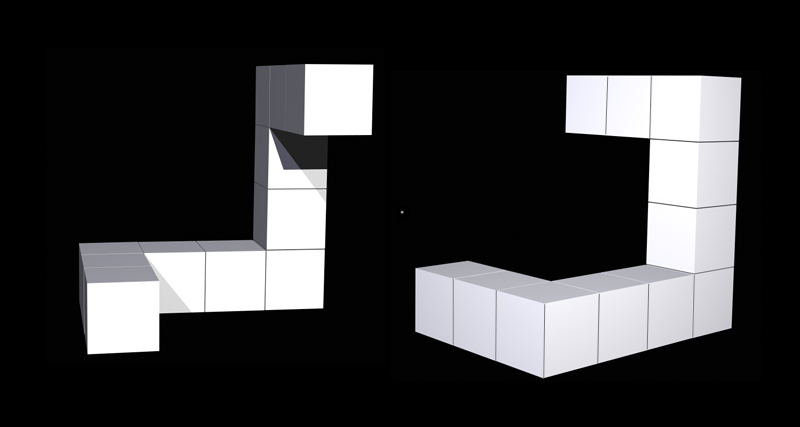
\includegraphics[width=0.45\columnwidth]{chapter4_fig/rotation_example.jpg}
		\caption{A typical example of a rotated 3D objects card.} 
		\label{fig:rotation_task_exp2}
	\end{figure}
	
For each human test subject, three different control modes were tested. In \textbf{\textit{teleoperation}} mode, the operator was restricted to using only direct joystick control to steer the robot, and no use of the robot's autonomous navigation capabilities was allowed at any time. In \textbf{\textit{autonomy}} mode, the operator was only allowed to guide the robot by clicking desired destinations on the 2D map. The only exception was in the case of critical incidents such as the robot becoming stuck in a corner. Under such circumstances the experimenter would instruct the human operator to briefly revert to joystick control in order to free the robot so that the experiment could continue. In \textbf{\textit{Human-Initiative (HI)}} mode, the operator was given freedom to switch LOA at any time (using a push-button on the joy-pad) according to their judgment, in order to maximize performance. 

\subsection{Participants and procedure}
A total of 24 test subjects participated in a within-groups experimental design (i.e. every test subject performed all three trials), with usable data from 23 participants. A prior experience questionnaire revealed that the majority of the participants were experienced in driving, playing video games or operating mobile robots. Each test subject underwent extensive training before the experiment. This ensured that all participants had attained a common minimum skill level (which otherwise might lead to a confounding factor in later data analysis). Participants were not allowed to proceed with the experimental trials until they had first demonstrated that they could complete a training obstacle course three times, within a specific time limit, with no collisions and while presented with the two degrading factors (i.e. the secondary task and sensor noise). Each of the three training trials used a different control mode. Additionally, all participants were required to perform the secondary task separately (i.e. without driving the robot) in order to establish baseline performance.

During the actual experimental trials (testing the three different control modes), counterbalancing was used, i.e. the order of the three control modes was rotated (through six different possible permutations) for different participants. The purpose of this counterbalancing measure was to prevent both learning and fatigue effects from introducing confounding factors into the data from a within-groups experiment. Ideally, counterbalancing should have been done using 24 test-subjects (i.e. a multiple of 6). Unfortunately, due to technical reasons, only 23 out of our 24 human test-subjects yielded usable data, however our slightly imperfect counterbalancing over 23 subjects should still have eliminated most learning and fatigue effects from our statistical results. For the secondary task, different cards, but of equal difficulty \citep{Ganis2015}, were chosen randomly before each trial, again to eliminate learning as a confounding factor in the test data. 

Participants were instructed to perform the primary task (controlling the robot to reach a destination) as quickly and safely (i.e. minimizing collisions) as possible. Additionally they were instructed that, when presented with the secondary task, they should do it as quickly and as accurately as possible. They were explicitly told that they should give priority to the secondary task over the primary task and should only perform the primary task if the workload allowed. Also they were told that there would be a score penalty for every wrong answer. This experimental procedure was informed by initial pilot study tests, with pilot participants, which showed that when people are instructed to ``do both tasks in parallel to the best of your abilities'', they  either a) ignore the secondary task or b) choose random answers for the secondary task to alleviate themselves from the secondary workload, so that they can continue focusing on the primary task of robot driving. Lastly, participants were informed that the best performing individuals in each trial (using a weighted performance score based on both primary and secondary tasks) would be rewarded with a gift voucher. The purpose of this prize was to provide an incentive for participants to achieve the best score possible on both primary and secondary tasks.

The human operators can only acquire situational awareness information via the Operator Control Unit (OCU) which displays real-time video feed from the robot's front-facing camera, and displays the estimated robot location (derived from laser scanner and SLAM algorithm) on the 2D SLAM map.

Our previous work (see \citep{Chiou2015} or Section \ref{chap3:guidelines}) showed that a difficult confounding factor can be introduced by the fact that different test subjects may explore in different directions, thus revealing different information about the test arena at different times, as the robot's onboard laser SLAM progressively performs mapping. Additionally, real-time SLAM can produce maps of varying accuracy between trials. To overcome this confounding factor, all participants were given an identical and complete 2D map, generated offline prior to the trials by driving the robot around the entire arena and generating a complete SLAM map.

During each trial, a variety of data and metrics were collected: primary task completion time (time taken for the robot to travel from point A to point B and back again to point A (see Fig.\ref{subfig:map_exp2}); total number of collisions; secondary task completion time; number of secondary task errors. At the end of each experimental run, participants had to complete an online NASA Task Load Index (NASA-TLX) \citep{Sharek2011}  questionnaire. 

\section{Human-Initiative system performance analysis}

Statistical analysis was conducted on a number of metrics gathered during the experiments. A repeated measures one-way ANOVA was used, with a Greenhouse-Geisser correction in the cases that sphericity assumption was violated (i.e. that the variances of the differences between conditions/levels are not equal). The independent variable was the control mode with three levels, i.e. autonomy; teleoperation; and HI. Fisher's least significant difference (LSD) test was used for pairwise comparisons given the a) clear hypothesis; b) predefined post-hoc comparisons; c) small number of comparisons. LSD is typically used after a significant ANOVA result to determine explicitly which conditions differ from each other through pairwise comparisons. Here we consider a result to be significant when it yields a $p$ value less than $0.05$, i.e. when there is less than a 5 percent chance that the observed result occurred merely by chance. We also report on the statistical power of the results. Power denotes the probability that a statistical significant difference will be found, if it actually exists. It is generally accepted that greater than 80 percent chance to find such differences constitutes a good power value. Lastly $\eta^2$ is reported as a measure of effect size.

\subsection{Results}\label{chapter4:results_system}
% PRIMARY TIME
ANOVA for \textit{primary task completion time} (see Fig. \ref{subfig:totalTime_exp2}) showed overall significantly different means with \textit{F(1.275, 28.057) = 34.567,  $p < .01$, $power > .9$, $\eta^2 = .61$} between HI variable-autonomy (\textit{$M = 413.6$ $sec$, $SD = 33.7$}), autonomy (\textit{$M = 483.9$ $sec$, $SD = 45.4$}) and teleoperation (\textit{$M = 429.6$ $sec$, $SD = 45.7$}). Pairwise comparison reveals that pure autonomy performed significantly worse (i.e. higher mean completion time) than the other two modes of operation with \textit{$p <.01$}. Also HI variable autonomy performed significantly better (i.e lower mean completion time) than teleoperation (\textit{$p <.05$}). 

% COLLISIONS
The effect of control mode on the number of \textit{collisions} (see Fig. \ref{subfig:totalCollisions_exp2}) was significant, \textit{F(1.296, 28.507) = 9.173, $p < .05$, $\eta^2 = .29$} with a \textit{$power > .85$}. Pure autonomy mode led to significantly (\textit{$p < .05$}) fewer collisions (\textit{$M = .61$, $SD = .89$}) than teleoperation (\textit{$M = 2.43$, $SD = 2.78$}). HI variable autonomy mode (\textit{$M = .57$, $SD = .99$}) also led to fewer collisions (\textit{$p < .01$}) than teleoperation. HI and autonomy had no significant difference. Playback of the recorded trials revealed that in teleoperation most of the collisions occurred during the time of the secondary task. This was true for the participants that attempted to perform both tasks in parallel as they were not able to allocate enough attention in safely operating the robot. This is indicative of the performance degradation effect that the secondary task had on the primary.

	\begin{figure}
		\centering
		\begin{subfigure}[b]{0.49\textwidth}
			\centering
			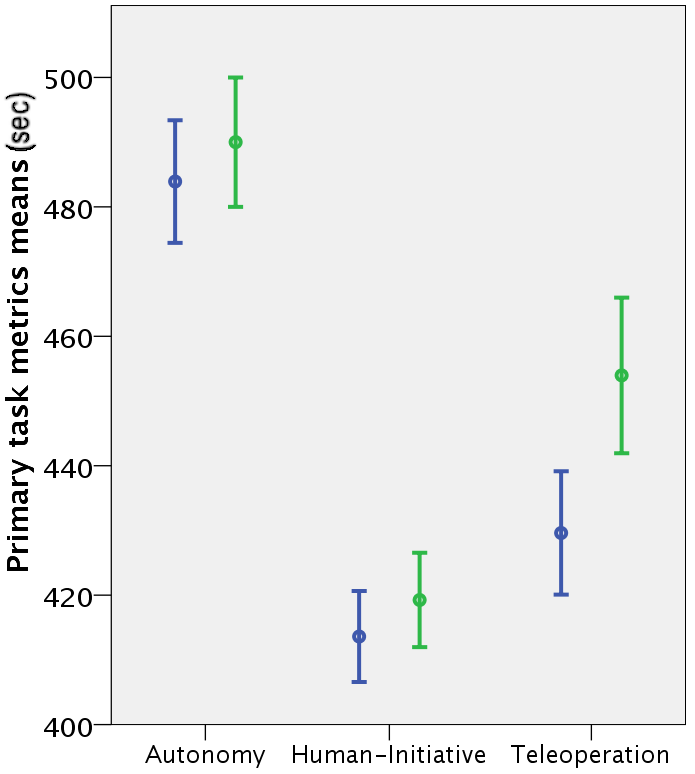
\includegraphics[width=\textwidth]{chapter4_fig/primary_metrics_time.png}
			\caption{}
			\label{subfig:totalTime_exp2}
		\end{subfigure}
		\hfill
		\begin{subfigure}[b]{0.49\textwidth}
			\centering
			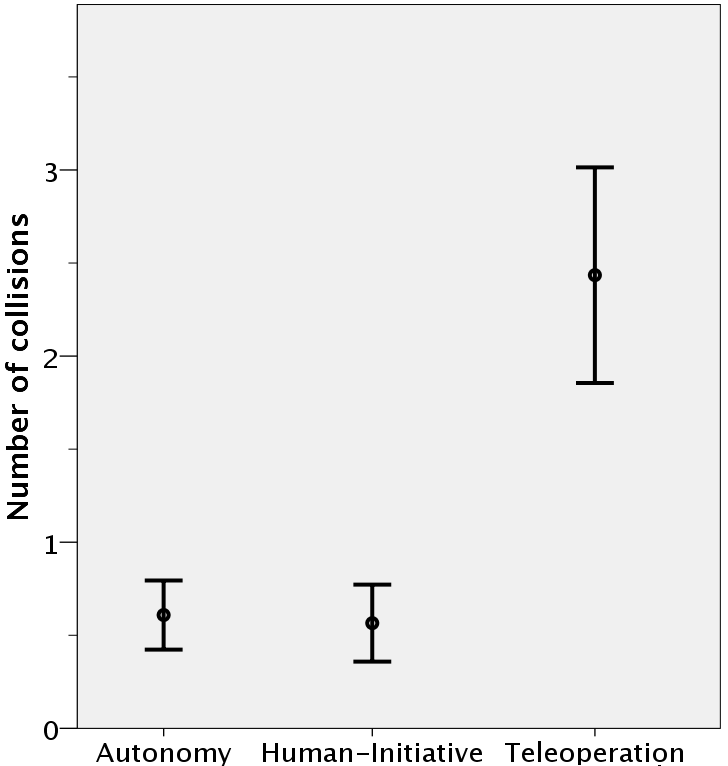
\includegraphics[width=\textwidth]{chapter4_fig/collisions.png}
			\caption{}
			\label{subfig:totalCollisions_exp2}
		\end{subfigure}
		\hfill
		\caption{Primary task results. \textbf{\ref{subfig:totalTime_exp2}:} average time to completion (blue) and score combining time and collisions penalty (green). \textbf{\ref{subfig:totalCollisions_exp2}:} average number of collisions. In all graphs the error bars indicate the standard error.}
		\label{fig:time_collisions_exp2}
	\end{figure}
	
% PRIMARY SCORE
It is useful to be able to rank each trial according to an overall performance metric, which we refer to as the \textit{primary task score}. This overall score is needed to be able to compare e.g. one human operator who achieves a very fast task completion time, but with many collisions, against another operator who achieves a slower time but with few collisions. We generate the primary task score by adding a time penalty of \textit{$10$ $sec$} for every collision onto the primary task completion time for each participant. This is inspired by the performance scores used in the RoboCup competitions \citep{Jacoff2003a}. Fig. \ref{subfig:totalTime_exp2} shows the mean primary task scores for each robot control mode. ANOVA analysis confirmed that control mode had a significant effect on the primary task score, \textit{F(1.336, 29.403) = 19.342, $p < .01$, $power > .95$, $\eta^2 = .47$}. LSD test suggests that HI variable autonomy (\textit{$M = 419.2$, $SD = 35$}) significantly (\textit{$p <.01$}) outperforms both the pure autonomy mode (\textit{$M = 490$, $SD = 47.93$}) and the pure teleoperation mode (\textit{$M = 453.9$, $SD = 57.68$}). Note also that teleoperation appears to outperform autonomy (\textit{$p <.05$}) in these experiments. This is due to the different amounts of degradation from the added noise. The laser noise stops the robot. The secondary task slows or in some cases completely stops the human.

% SECONDARY TIME
\textit{Secondary task completion time} (see Fig. \ref{subfig:secondary_time_exp2}) refers to the average time per trial that the participants took to complete one series of the 3D object cards. ANOVA with \textit{$F(1.565, 34.420) = 7.821, p < .01 , power > .85$, $\eta^2 = .26$}, suggests that there is a significant difference between the mean secondary task completion times with and without also performing the primary task of controlling the robot. Participants performed significantly ($p < .05$) better in the baseline trial (\textit{$M = 33.2$ $sec$, $SD = 5.52$}) compared to their performance during robot operation. During robot operation, HI variable autonomy mode (\textit{$M = 39.3$ $sec$, $SD = 10.35$}), pure autonomy mode (\textit{$M = 39.5$ $sec$, $SD = 12.32$}) and teleoperation mode (\textit{$M = 41.7$ $sec$, $SD = 16.5$}) did not show statistical differences.

	\begin{figure}
		\centering
		\begin{subfigure}[b]{0.49\textwidth}
			\centering
			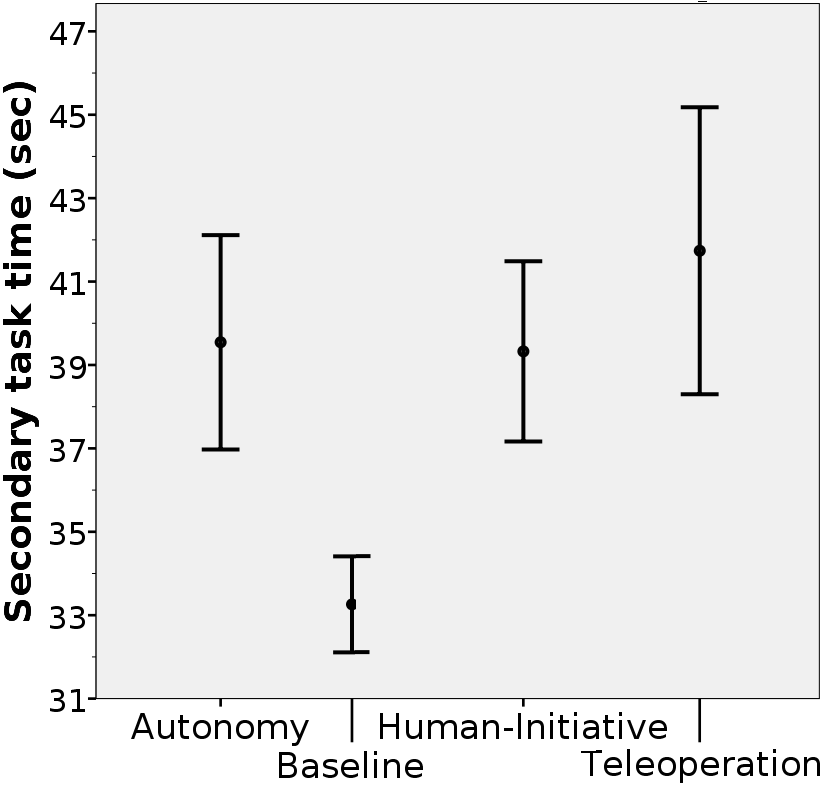
\includegraphics[width=\textwidth]{chapter4_fig/secondary_time.png}
			\caption{}
			\label{subfig:secondary_time_exp2}
		\end{subfigure}
		\hfill
		\begin{subfigure}[b]{0.49\textwidth}
			\centering
			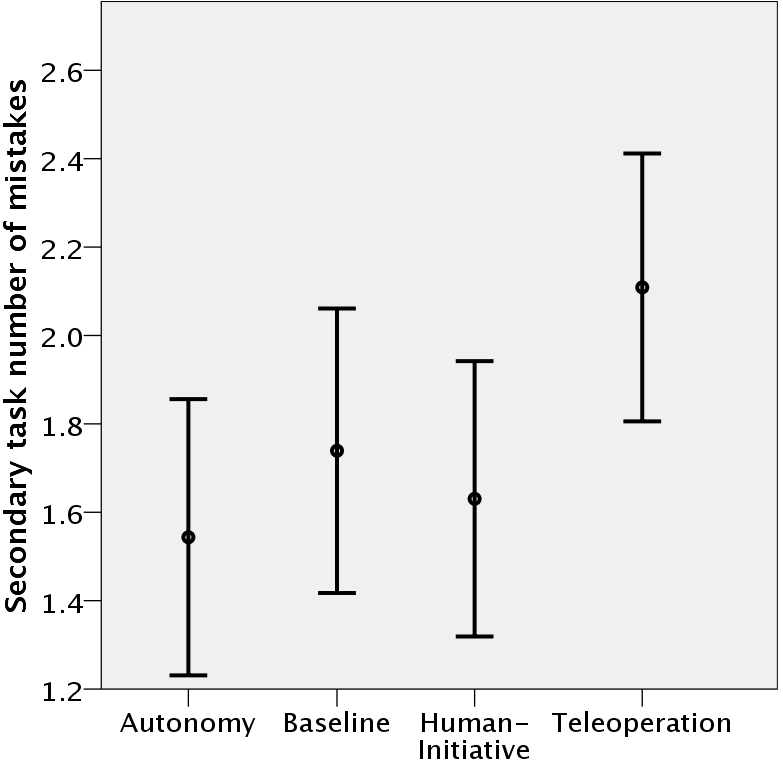
\includegraphics[width=\textwidth]{chapter4_fig/secondary_mistakes.png}
			\caption{}
			\label{subfig:secondary_mistakes_exp2}
		\end{subfigure}
		\hfill
		\caption{Secondary task performance. \textbf{\ref{subfig:secondary_time_exp2}:} average time to completion for one series of 3D objects. \textbf{\ref{subfig:secondary_mistakes_exp2}:} average number of errors for one series of 3D objects.}
		\label{fig:rt_exp2}
	\end{figure}

% SECONDARY MISTAKES
No significant differences were observed between the different robot control modes with respect to numbers of secondary task errors (see Fig. \ref{subfig:secondary_mistakes_exp2}) according to ANOVA with \textit{$F(3,66) = 1.452, p > .05 , power < .8$, $\eta^2 = .06$}. Participants had \textit{$M = 1.74$, $SD = 1.54$} errors during baseline tests without operating the robot, \textit{$M = 1.63$, $SD = 1.49$} during HI variable autonomy mode, \textit{$M = 1.54$, $SD = 1.49$} in pure autonomy mode, and \textit{$M = 2.1$, $SD = 1.45$} in pure teleoperation mode.

% NASA-TLX
Control mode had a significant effect on \textit{NASA-TLX scores} (see Fig. \ref{fig:NASA-TLX_exp2}) as suggested by ANOVA (\textit{$F(2,44) = 11.510, p < .01 , power > .9$, $\eta^2 = .34$}). Pairwise comparisons showed that autonomy (\textit{$M = 35.2$, $SD = 11.83$}) was perceived by participants as having the lowest difficulty, as compared to HI variable autonomy mode (\textit{$M = 41.4$, $SD = 12.67$}) with $p < 0.05$ and teleoperation mode (\textit{$M = 47.8$, $SD = 11.87$}) with $p < 0.01$. HI variable autonomy is perceived as being less difficult than teleoperation ($p < 0.05$). 

\begin{figure}
	\centering
	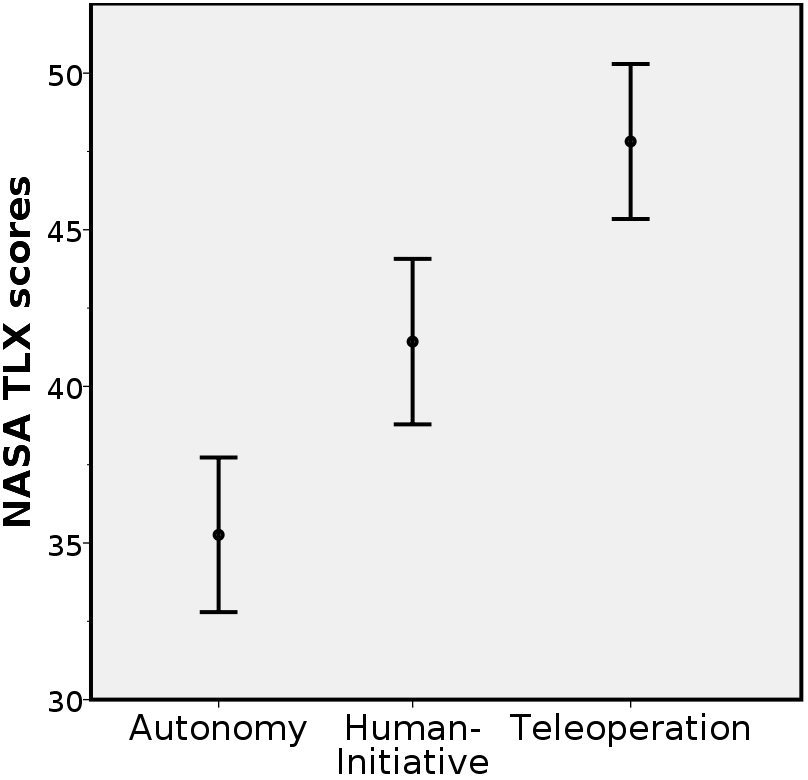
\includegraphics[width=0.49\columnwidth]{chapter4_fig/NasaTLX.png}
	\caption{NASA-TLX score showing the overall trial difficulty as perceived by the operators.} 
	\label{fig:NASA-TLX_exp2}
\end{figure}

\subsection{Discussion}

In terms of overall primary task performance, HI variable autonomy control significantly outperformed both pure teleoperation and pure autonomy. This confirms our hypothesis that a variable autonomy system with the capability of on-the-fly LOA switching can improve overall performance of the human-robot team. In essence, it does so by being able to overcome situations in which a single LOA may struggle to cope. For example, external distractions to the operator such as the secondary task can be overcome by the operator switching from teleoperation to autonomy. In contrast, when autonomous control struggles to cope with noisy sensory information, the situation can be ameliorated by switching to teleoperation. From the Human-Robot Interaction (HRI) perspective, operators were able to successfully change LOA on-the-fly in order to maximize the system's performance. Since the LOA change was based on the operator's judgement, these experiments suggest that, given sufficient training, operators make efficient use of the variable autonomy capability. Additionally, note that autonomy generates significantly fewer collisions than teleoperation, however HI variable autonomy generates equally few collisions. This reinforces the conclusion that human operators can efficiently exploit autonomy by making smart decisions about switching between autonomy and teleoperation when most appropriate. 

Regarding the secondary task, when performed in isolation from the primary task (during baseline testing), participants perform better. Since participants were instructed to focus on the secondary task whenever it was presented, this suggests that even having the primary task waiting on standby was enough to impair their performance on the secondary task. The absence of statistical differences across control modes in the secondary task time to completion and errors, suggests that a) the choice of control mode did not have any effect on secondary task performance; b) participants had the same level of engagement with the secondary task across trials.

NASA-TLX showed that autonomy is perceived as the easiest control mode, while HI is perceived as being easier than teleoperation. The fact that HI is perceived as more difficult than autonomy might perhaps reflect the cognitive overhead imposed on the operator by having to make judgements about switching LOA. This suggestion was further reinforced by observations made during trials and from informal conversations with participants. Most participants demonstrated a more laid-back attitude while using autonomy. However, participants stated that, while HI variable autonomy mode was ``more stressful and demanding'', it was also ``more fun'' due to a perception of increased engagement. For this reason, many participants expressed strong preference for HI variable autonomy over the other control modes. These observations are perhaps related to those of \citep{Wen2015} which suggests that humans' ``sense of agency'' is improved when they interact more actively with a system.

\section{Human-Initiative Human-Robot Interaction analysis}
Here, we present data and analyses regarding the ways in which human operators interacted with the dynamic LOA switching capabilities of the HI system. The percentage of time spent in each LOA (i.e. teleoperation or autonomy) during the HI trials was measured. We report mostly on the time spent in the autonomy LOA, because: firstly, it was the dominant LOA chosen by human test-subjects during the HI trials; secondly, everything that is correlated (or not) with percentage of time in autonomy is also inversely correlated (or not) with percentage of time in teleoperation LOA. This is due to the fact that these two modes combine together to form almost $100\%$ of the time of each trial. The remaining small percentage of time corresponded to a ``stop mode'' which allows operators to perform emergency canceling of navigational goals and robot movement. 

\begin{figure}
		\centering
		\begin{subfigure}[b]{0.5\textwidth}
			\centering
			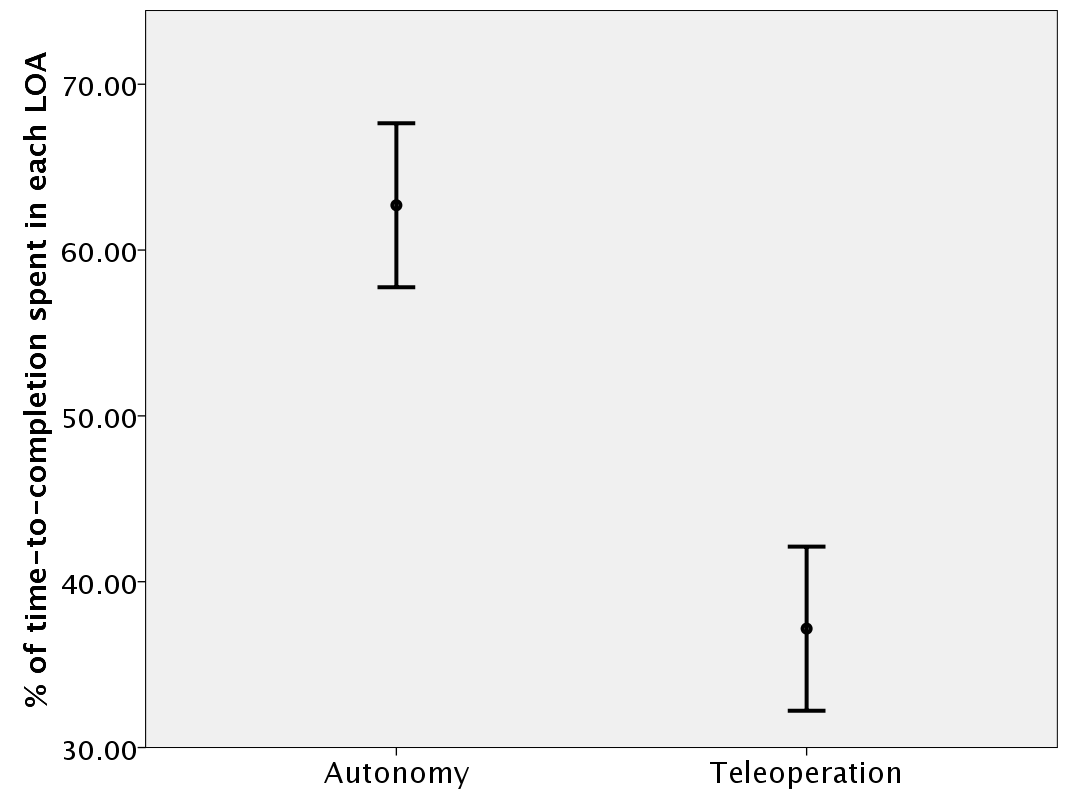
\includegraphics[width=\textwidth]{chapter4_fig/time-in-mode.png}
			\caption{}
			\label{subfig:time-percentage-mode_exp2}
		\end{subfigure}
		\hfill
		\begin{subfigure}[b]{0.45\textwidth}
			\centering
			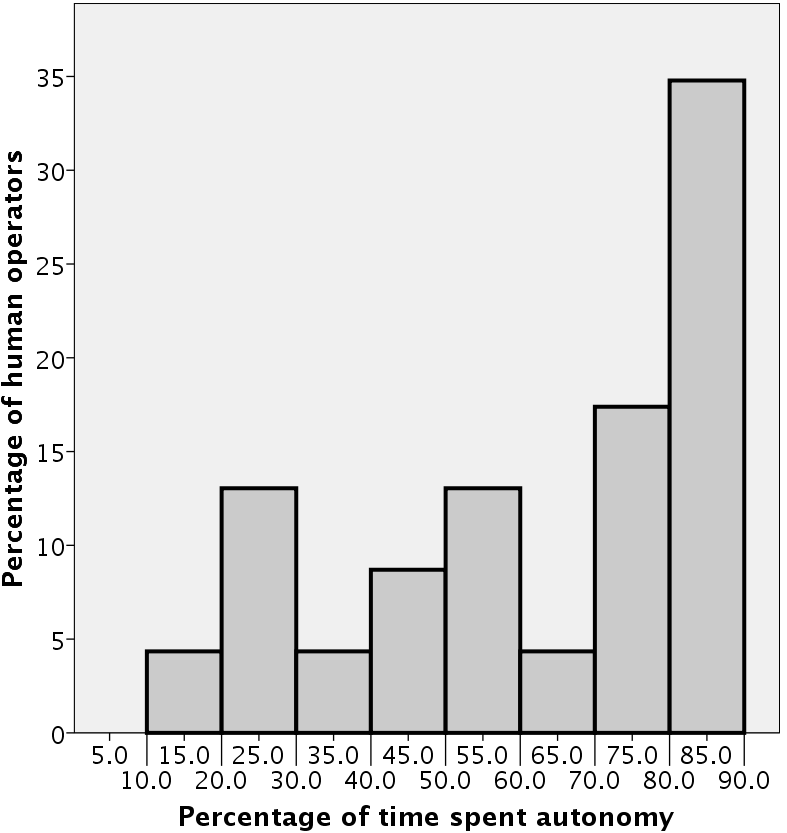
\includegraphics[width=\textwidth]{chapter4_fig/time-mode-histogram.png}
			\caption{}
			\label{subfig:time-percentage-histogram_exp2}
		\end{subfigure}
		\hfill
		\caption{\textbf{\ref{subfig:time-percentage-mode_exp2}:} Percentage of time-to-completion spent in each of the two LOAs during the HI trials. Error bars indicate the standard error. \textbf{\ref{subfig:time-percentage-histogram_exp2}:} Histogram showing the proportion of human operators who spent various different proportions of their time in the autonomy LOA during HI experiments.}
		\label{fig:time-percentage_exp2}
\end{figure}

\subsection{Results}
\label{chapter4:results_HRI}
The average percentage of time spent in teleoperation mode was \textit{$M = 37.17\%$} and the average time spent in autonomy was \textit{$M = 62.7\%$}, see Fig. \ref{subfig:time-percentage-mode_exp2}. The standard deviation, across trials, on these percentages was $SD = 23.7$. The remaining $0.13\%$ of time was spent in stop mode. As can be seen in the histogram (see Fig. \ref{subfig:time-percentage-histogram_exp2}) the majority of the human test-subjects spent more than 60\% of the time using autonomy. Additionally there were two other smaller groups of operators based on Fig. \ref{subfig:time-percentage-histogram_exp2}. One group equally split their time between autonomy and teleoperation, while the third group mostly (i.e. more than 60\% of the time) chose to use the teleoperation mode.

% Frequancy of switchies
The number of LOA switches operators performed in each trial denotes the frequency in which they make use of the HI controller capabilities. The mean number of LOA switches per trial was  $M = 9.78$ with a standard deviation of $SD = 7.367$. As can be seen from the histogram of Fig. \ref{fig:number-loa-switches_exp2}, the vast majority of the operators (more than 74\%) changed LOA fewer than 11 times. A much smaller number of operators choose to switch control very often (more than 16 times per trial).


\begin{figure}
	\centering
	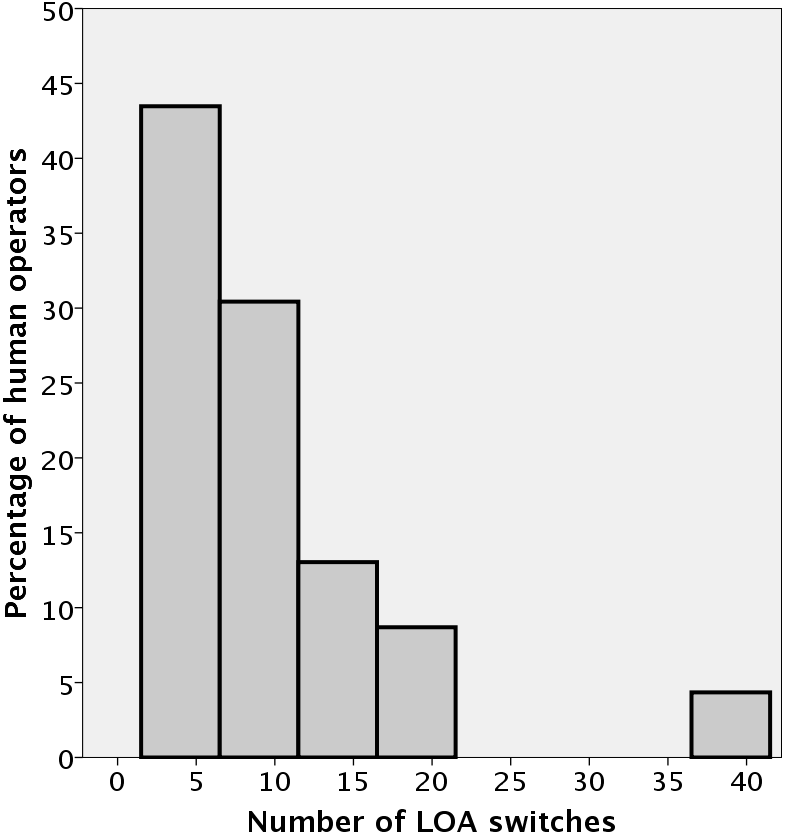
\includegraphics[width=0.49\columnwidth]{chapter4_fig/number-loa-switches.png}
	\caption{Histogram showing the percentages of human operators who chose to make various different numbers of LOA switches during HI trials.} 
	\label{fig:number-loa-switches_exp2}
\end{figure}

% Correlations performance + number of LOA switches
Correlation analysis using a two-tailed Pearson's $r$ was conducted to investigate any relationships between human-robot team performance and other variables. Firstly the \textit{number of LOA switches} and the \textit{percentage of time spent in autonomy} were not correlated $r(21)= .24, p>.05 $. No correlation was found between the \textit{number of LOA switches} and performance of the system in terms of \textit{primary task time-to-completion} (duration of navigation from A to B and back), $r(21)= -.43, p>.05 $. Also there was no correlation between the \textit{number of LOA switches} and performance in the \textit{secondary task completion time}, $r(21)= .016, p>.05$. The \textit{percentage of time spent in autonomy} and performance in the \textit{primary task time-to-completion}, were not correlated $r(21)= .012, p > .05$. Lastly, the \textit{percentage of time spent in autonomy} was not found to be correlated with the \textit{secondary task completion time}, $r(21)= .16, p>.05$.

% NASA-TLX
In \textit{NASA-TLX} scores (see section \ref{chapter4:results_system}), ANOVA and pairwise comparisons showed that autonomy was perceived by participants as having the lowest difficulty, as compared to HI and teleoperation. Correlation analysis showed that \textit{NASA-TLX scores} were inversely and significantly correlated with the \textit{percentage of time spent in autonomy} during the HI trials, $r(21)= -.446, p < .05$. The greater the proportion of time spent in autonomy mode, the easier the task was perceived to be by the human test-subjects. Analysis found no correlation between the \textit{number of LOA switches} and \textit{NASA-TLX scores}, $r(21)= -.016, p < .05$.

\subsection{Discussion}
The analysis showed that the majority of the participants chose to use mostly autonomy mode. Furthermore, participants switched LOA $9.78$ times on average. The fact that there is no correlation between either of those two factors and performance in primary or secondary tasks, suggests that operators used LOA switching for reasons that are not purely related to task performance. However, our previous work in \citep{Chiou2016} and Section \ref{chapter4:results_system} did clearly demonstrate that HI variable autonomy can outperform pure autonomy or pure teleoperation in various situations. Thus, it can be inferred that part of the time spent in autonomy, and a number of the observed LOA switches, were crucial in improving overall task performance. This in turn, suggests that all participants attained a minimum skill level to successfully exploit the HI LOA switching capabilities, further reinforcing the findings.

The remaining use of autonomy and number of LOA switches (i.e. those in excess of what were needed to achieve good performance), may simply reflect personal preferences. These individual preferences can be driven by several factors. The level of trust in the autonomous control can lead operators to use more or less autonomy. For example, a test-subject who does not trust the robot's autonomous capabilities, may choose rely on direct teleoperation more than is necessary. Since, in our experiments, the autonomy mode was highly used by most test-subjects, this suggests that human operators did indeed trust that the robot's autonomous navigation AI will perform at least as well as a human teleoperator in most situations.

Operators' personality traits may also play an important role. Possibly some humans prefer to be more in control of a situation or show a more hands-on attitude, and are therefore likely to use more teleoperation. Others may prefer the role of a supervisor in conjunction with a more laid back attitude. Those individuals are likely to use more autonomy. Additionally, note that a number of LOA switches can be traced to the general alertness of human operators, triggered by their anticipation of events. For example, some operators may switch preemptively to autonomy while anticipating the appearance of a secondary task. Other operators may switch preemptively to teleoperation if they anticipate the robot getting stuck in an awkward situation in the test arena. The latter was observed by the experimenters in a number of participants, who would switch momentarily to teleoperation in parts of the arena where they felt the robot was performing sub-optimally, e.g. while navigating around sharp corners. These participants tend to switch LOA more frequently and thus fall into the group of operators with a very high number of LOA switches, see Fig. \ref{fig:number-loa-switches_exp2}. 

Correlation between NASA-TLX scores and the percentage of time spent in autonomy, shows that participants who mostly used the autonomy mode perceived the overall task and operational difficulty to be easier than those who used mostly teleoperation. Firstly, this further validates the NASA-TLX results in Section \ref{chapter4:results_system} that found autonomy to be easier than teleoperation. However, it is still not clear if the causal reason that operators preferentially chose autonomy more than teleoperation is because they perceived it as an easier and more effective control mode. Further investigation is needed to confirm cause and effect. Secondly, it is a possible indication of the extra cognitive overhead that switching LOA based on judgment may impose on the operator. In particular while teleoperating or while occupied with a secondary task, the operator can find himself in an overwhelming situation. Thus, he/she may find it difficult to judge which is the appropriate LOA for the situation or he/she may be too overwhelmed to actually perform the LOA-switching action (i.e. making a cognitive decision to switch, followed by executing a button press). This problem of cognitive overloading of the human operator, can be tackled by implementing a Mixed-Initiative (MI) robotic system in which both the AI and the human operator have the authority to initiate LOA changes. The AI can assist by taking control from the operator or switching LOA while he/she is occupied, thus alleviating him/her from the burden of manual control.


\section{Conclusions and impact}
\label{chap4:conclusion} 
This chapter presented a systematic and statistically validated empirical analysis of a variable autonomy robot control system. Previously, a comparatively small part of the robotics literature has addressed the issues of variable control. Previous studies have focused on the engineering and computer science behind building such systems or on enhancing the human-robot control interface. 

In contrast to the literature, this chapter has made a variety of new contributions, including: showing how to carry out a principled performance evaluation of the combined human-robot system, with respect to completing the overall task; presenting clear empirical evidence to support the notion that variable autonomy systems may have advantages over purely autonomous or teleoperated systems for certain kinds of tasks; using rigorous methodologies, transferred from the fields of psychology and human factors research, to inform experimental design, eliminate confounding factors, and yield results that are statistically validated; and demonstrates that human operators, when appropriately trained, make successful decisions about switching LOA, which efficiently exploit the contrasting strengths of both teleoperation and autonomous controllers. We must note here that our hypothesis and experimental paradigm are intended to be a starting point, from which more complex hypotheses and scenarios can be formulated.

In the HRI dimension of HI control, the analysis was focused on the use of the dynamic mode-switching capabilities of the system by the operator. We believe this is the first study which has quantitatively reported on metrics such as percentage of time spent in each LOA, frequency of LOA switches, and perceived workload and difficulty in regard to such metrics. 

Overall, we believe this is the first study which has used a systematic and repeatable framework to support the continued development of variable autonomy mobile robots. 


\chapter{DESIGN AND EVALUATION OF A MIXED-INITIATIVE CONTROL SYSTEM}
\label{chapter5:MI}
In this chapter we build on our previous work (see Chapters \ref{chapter3:towards} and \ref{chapter4:HI}) in order to progress research towards designing Mixed-Initiative controllers, conducting systematic experimental evaluations of MI control, and identifying the major challenges that MI research needs to overcome. In brief, this is done by describing the design of two MI controllers and then reporting on two evaluation experiments for one of the controllers. The first experiment was in a simulated environment while the second one took place in a controlled real world environment. When evaluating novel systems, using both real and simulated environments has the benefit of providing comprehensive insights. Simulated environments are ideal for initial evaluations as they are easily controlled and thus minimize confounding factors. The benefit is that the fundamental principles of the system under evaluation can be tested with a high degree of confidence. Real world experiments on the other hand are ideal for follow up evaluations as they introduce realism and a less sterilized environment (i.e more confounding factors). Thus, the robustness of the system can be tested in a variety of conditions (e.g. different environment layout, unforeseen performance degrading factors etc).

Initially, we discuss the difficult issues involved in extending notions of variable autonomy from Human-Initiative (HI) to Mixed-Initiative (MI) robotic systems. Towards this end we propose an approach to designing expert-guided MI controllers. This approach is informed by our previous experiments. Then, using this approach and data from our previous experiments, we design a novel fuzzy MI controller. This controller is novel for the following reasons, as elaborated in our literature survey (see Sections \ref{section:MI-taxonomy} and \ref{section:MI-systems}): a) it is the first MI controller that is capable of LOA switching during task execution; and b) the first to be practically implemented and experimentally evaluated. Additionally, we took a novel approach in designing the MI controller as it makes use of expert knowledge; an online performance metric; and simplified context knowledge. 

The fuzzy MI controller is evaluated in two different experimental settings. First, we conduct a replication of the experiment reported in Chapter \ref{chapter4:HI} in order to make an initial evaluation of the MI controller. The performance of the MI controller is compared with the performance of the HI controller. Evidence is reported showing that the MI controller can outperform HI in terms of navigation task performance under various circumstances. Moreover, evidence shows the potential advantages of MI regarding mentally demanding secondary tasks such as mental rotation of 3D objects. Lastly, results from this initial experiment show the potential benefits of MI control in alleviating operator's workload.

Our experimental framework is also extended into a more complex and realistic real world scenario. An experiment is presented which was designed to evaluate how the MI controller would perform in a real robot used in an Urban Search and Rescue (USAR) scenario. Some of the results comparing HI with MI proved hard to interpret conclusively. However, this problem itself yielded interesting new insight into two major challenges for MI systems. Lastly, the experiment provided real world evidence, in contrast to our previous experiment using a simulator, further demonstrating the advantages of HI variable autonomy when compared with teleoperation.

\section{Framework for designing an expert-guided Mixed-Initiative robotic system}
\label{chapter5:general_expert_MI}

The fundamental problem of MI in the context of this thesis is the LOA switching by either the operator or the robot controller in order to improve the human-robot system's performance (e.g. by overcoming a performance degrading factor). The robot, in this case meaning the hardware, can be seen as a resource with two different agents having control rights: one agent is the human operator and the other is the robot's autonomous control system (i.e. the robot controller). At any given moment, the most capable agent should take control. Hence, of particular importance is the ability of each agent to diagnose the need for a LOA change, and to take control (or hand over control) successfully.

An operator's LOA switches are based on judgment. As demonstrated by the HI results presented in Chapter \ref{chapter4:HI} (see also results presented in this chapter), humans are able to diagnose when they need to intervene, given sufficient understanding of the system and the situation. More specifically, empirical observations and careful analysis of the HI results from our previous work (see Chapter \ref{chapter4:HI} and \citep{Chiou2016,Chiou2016_AAAI}) revealed that operators switch LOA based on three factors: a) preferred LOA; b) context; and c) performance degradation. The preferred LOA constitute participants' default LOA. For example some operators prefer autonomy over teleoperation. It reflects individual preferences based on a number of factors (e.g. trust in the AI) and personal traits (e.g. preference to be in control). In context sensitive LOA switches, operators are able to evaluate the current context and infer if a LOA switch is needed. For example they can change control preemptively as they predict performance degradation in a given situation. An example would be a situation in which noise starts to appear in the sensors, thus they change to teleoperation as they predict degradation in autonomy's performance.

On the other hand, it is not obvious how to enable the robot controller to detect when the performance of the system is degraded. This is necessary to enable the robot controller to robustly and automatically take control when it is needed and to relinquish control when under-performing. For example, the robot controller can initiate a switch to a LOA that offers increased autonomous capabilities. This can be beneficial in situations where the human operator is too preoccupied with the primary cause of his or her performance degradation to voluntarily switch control to the robot. Compared to a human operator the robot controller does not have personal preferences. Also, an AI system able to understand and take context sensitive decisions can be complex and challenging to design. Thus, in order to inform the design of MI robotic systems we focus primarily on LOA switches based on task performance degradation. 

To this end we propose the expert-guided approach on designing MI controllers. In the core of our proposed approach is the following assumption: given a task, we assume the existence of an "expert" controller which is able to control the robot in a close-to-optimal manner in that task. Based on this assumption, the core idea is that the MI controller should compare the current performance of the system with the expert performance. This comparison will yield an online \textit{task effectiveness} performance metric. In essence this metric should express how effective the system is performing in a given task, compared to the close-to-optimal performance of an expert in the same task. Any robot initiative on switching LOA should be based on that metric. For example if the system is not performing as effective in the task compared to the expert then the robot controller should initiate a LOA switch.

The expert-guided MI controller approach proposed here relies on the following assumptions: a) human operators are willing to either be handed control or hand over control; b) the agent to which the control will be traded or the LOA selected, is capable of coping with the cause of performance degradation (see Section \ref{chap3:guidelines} or \citep{Chiou2015}); c) the system is equipped with expert knowledge or an expert controller providing information on how the system should be performing (i.e. close-to-optimal performance) in a given task. 

As we will discuss in the later sections, there are a variety of approaches on using expert knowledge or an expert controller when designing a MI system. For example, machine learning techniques can be exploited in order to learn patterns of how human operators efficiently change LOA. This can be achieved by using those techniques on HI data gathered during experiments. Alternatively or additionally, expert knowledge or heuristics can be encoded into a fuzzy logic controller capable of taking informed decisions on LOA switching.


\section{Designing the expert-guided Mixed-Initiative controller for navigation}
\label{chapter5:designing_MI_nav}

In the context of this thesis, the expert-guided MI controllers presented (i.e. the threshold controller and the fuzzy controller) are focused primarily on LOA switches based on navigational performance degradation. Given the navigation task, an online error metric expresses the effectiveness of \textit{goal directed motion}. This metric, \textit{goal directed motion error} (refereed to as "error" for the rest of the chapter), is the task effectiveness performance metric (as discussed in the previous section) for the navigation task. In the simplified case, this could be a function of speed towards achieving a desired goal position \citep{Olsen2003} or the number of collisions inside a thresholded time window. The general idea is that the metric should compare the current progress towards achieving a navigation goal (i.e. a waypoint), to a close-to-optimal progress towards achieving the same goal. 

We used a closed loop control system approach to aid the design of the MI controllers. In this paradigm an error signal is typically used to denote system's performance deviations from a desired state. The raw error signal is processed and filtered into a meaningful form e.g. noise free. The controller relies on that processed error signal to infer the status of the system and take the appropriate actions in order to maintain the desired state of performance. 

For our navigation task, the expert performance is provided by a concurrently active navigation system. This expert system uses a robust off-the-shelf expert navigation planner from the Robot Operating System (ROS) navigation stack \citep{Marder-Eppstein2010}. More specifically, the global shortest feasible path is calculated based on Dijkstra's algorithm \citep{Dijkstra1959}, while the local path and optimal velocities are calculated using the dynamic window approach algorithm \citep{dwa_planner}. This expert planner calculates at any given moment a close-to-optimal path towards the goal and the close-to-optimal velocity which the robot should be moving along this path. This is given robot's current state (e.g. pose) and the surrounding location. From this velocity we isolate the linear component of the $x$ axis (i.e. the axis denoting the forward/backward motion of the robot). This linear speed denotes the speed which the robot should be moving towards the goal, by either moving forward (i.e. positive speed) or backwards (i.e. negative speed). In order for the error to be yielded, this speed from the expert planner is constantly compared with the current linear speed (i.e. the linear velocity component) of the robot moving towards the goal. Their difference is the \textit{goal directed motion error} that we use in the controllers presented in this chapter. Please refer to Fig. \ref{fig:block_diagram} for the block diagram of the system.

\begin{figure}
	\centering
	\includegraphics[width=0.8\columnwidth]{chapter5_fig/MIblockDiagram.png}
	\caption{The block diagram of the MI control system. Given a navigation goal; the current pose of the robot; and the map (or a known surrounding area); the expert planner yields a close-to-optimal suggested speed. This speed denotes how fast the robot should be moving towards achieving the navigation goal. Then this speed is compared with the current speed of the robot towards that goal to calculate the raw performance error. The MI controller decides on switching LOA based on the filtered error.} 
	\label{fig:block_diagram}
\end{figure}

In addition to the general assumptions described in the previous section, our navigation based MI controllers are following two additional assumptions: a) the map or the region surrounding the robot is known; and b) the system is equipped with a navigation expert planner capable of reliably computing both a close-to-optimal path and velocities towards a navigation goal.
 

\subsection{Threshold Mixed-Initiative controller}
\label{chapter5:threshold_controller}

Initially a threshold controller was designed based on the \textit{goal directed motion error} metric. More specifically, the controller models LOA switches initiated by the operators and which are based on their judgment about the current system performance. The model assumes the following two-step process: first it is observed over a period of time that the system's performance have dropped (e.g. based on a online metric). Second when this performance drop reaches a certain threshold, a switch in the LOA is initiated regardless on which agent is in control.

Based on our control engineering approach and our model, two requirements have to be satisfied by the error signal (i.e. the goal directed motion error) signal: a) frequent and very brief changes in error are considered as noise; b) the final error signal to be used should express the accumulated error over time. The first requirement comes from the fact that the error needs to be filtered into a meaningful noise free form. The second requirement comes from our model as it assumes that the performance drop is observed over a short period of time before any initiative takes place.

The exponential moving average (EMA) algorithm (frequently known as Brown's simple exponential smoothing \citep{Brown1963}) applied (see Equation \ref{eq:avg}) to the raw error (Equation \ref{eq:error}), satisfies both of these requirements. It acts as a smoothing filter to high frequency noise and also it accumulates the error over a period of time. It reflects the error trends quicker compared to a simple moving average as it does not have a phase shift. It is also easy to implement and computationally cheap. The raw error equation follows:

\begin{equation}\label{eq:error}
e_{t} = s_{E} - s_{R}
\end{equation}

The raw error $e_{t}$ is the difference between the close-to-optimal speed from the expert planner $s_{E}$ and the current linear speed $s_{R}$ of the robot moving towards the goal. The equation for the smoothed error using the EMA follows:

\begin{equation}\label{eq:avg}
E_{t} = \alpha \cdot e_{t} + (1-\alpha) \cdot E_{t-1}
\end{equation}

The term $E_{t}$ refers to the final accumulated and smoothed error. The term $e_{t}$ refers to the current error observation. The smoothing factor $\alpha$ controls the weight of the most recent (i.e. current) observation and thus the time window in which the error will be accumulated. The bigger the $\alpha$ is, the more the current error observation is taken into account and thus the smaller the accumulated error time window is (i.e. past error observations contributing less in the $E_{t}$ calculation). 

The threshold controller uses the filtered error $E_{t}$ to initiate LOA switches. When this error exceeds some threshold, the controller infers that the current agent in control is under-performing. Thus, it initiates a change in the LOA. The error threshold and the smoothing factor $\alpha$ parameters, were calculated using the following procedure: For every operator the HI data from the previous experiment (see Chapter \ref{chapter4:HI}) were run through the threshold controller. These data included the operator's LOA changes and their time-stamps, the speed of the robot and the performance error. For every operator the controller would yield a set of LOA switches predictions. In essence, the controller was attempting to match the LOA switches initiated by the operators on the previous HI data. A grid search algorithm was used to search and feed the controller with different parameters values. The cost function defined in Equation \ref{eq:cost_individual} was used on the controller's LOA switches predictions to calculate the cost of a particular parameters pair (i.e. the threshold and the $\alpha$) for each individual operator. The final parameters chosen, were the parameters that minimized the total (i.e. the sum) cost for all participants. The cost function for each individual follows:

\begin{equation}\label{eq:cost_individual}
j = \sum{|\hat{t^{i}_k} - t_k|} + c \cdot p
\end{equation}

Put simply, Equation \ref{eq:cost_individual} expresses the LOA switch prediction error from the controller on HI data, with the addition of a penalty term for every prediction that does not match (i.e. false positives). Where $\hat{t}$ is the time-stamp of the predicted LOA switch and $t$ is the time-stamp of the operator's actual switch. The subscript $k$ denotes a specific time-stamp. Where $c$ is the number of predictions that do not match operator's switches, and $p$ is a cost penalty. A non-matching prediction is defined a prediction that falls outside of a small time window around any of the operator's LOA switches. The assumption is that these predictions do not correspond to any actual operator's LOA switches and thus they get penalized. 

The parameters calculated with the grid search were $\alpha = 0.06$ and error $threshold = 0.07 m/sec$. We conducted a pilot experiment with a small number of participants, using these parameters with the threshold controller. It rapidly became clear that this controller did not work well. Poor performance was characterized by excessive LOA switching (i.e. the controller was oversensitive in detecting performance drops). As a result the controller was intrusive and impractical. This led us to design a new expert knowledge controller based on fuzzy logic, as described in the next section.

\subsection{Fuzzy Mixed-Initiative controller}
\label{chapter5:fuzzy_controller}
A bang-bang Mamdani type fuzzy controller \citep{Mamdani1975,Nagi2009} was designed to address the limitations of the threshold controller. In control theory a bang-bang controller (also known as on-off controller), is a controller that switches between two states. In this case, as explained later in this section, the controller's two states were: a) switch LOA; b) do not switch LOA. The Mamdani type refers to the type of the fuzzy inference process. In Mamdani inference \citep{Mamdani1975}, both the antecedent and the consequent parts of the fuzzy control rules are linguistic, allowing for expert knowledge to easily get incorporated into the system. Hence, the output after the linguistic fuzzy rules aggregation is a fuzzy set and needs defuzzification. Fuzzy rules aggregation is the process by which the fuzzy sets denoting the activation of each rule are combined to produce a single output fuzzy set. 

This controller constitutes an improvement compared to the previous simple threshold controller by utilizing expert knowledge in three ways: a) by defining fuzzy sets for the goal directed motion error, instead of a fixed threshold; b) by incorporating very simple context information; c) by taking informed decisions on when to initiate a LOA switch based on a fuzzy logic rule base. The hypothesis is that the fuzzy logic MI controller will yield smoother transitions between LOA switches decisions. Thus, will not be as intrusive (i.e. reactive) in switching LOA compared to the simple threshold controller.

In fuzzy logic a linguistic variable associates a linguistic concept and the fuzzy set representing that concept, to a numerical value. For example the linguistic variable "error" when its value is "small", associates the numerical value for "small" with the fuzzy set representing the concept of "small", i.e. with the membership function of "small" fuzzy set. Our fuzzy controller has two variables as inputs. The first linguistic input variable is "error" that denotes the filtered error. This is the filtered error from the exponential moving average (EMA) as in the previous threshold controller. The smoothing factor $\alpha$ used in the EMA filter, was the one found by the parameters search for the threshold controller. The second input variable is "speed" that denotes the speed in which the robot is currently moving. 

\begin{figure}
		\centering
		\begin{subfigure}[b]{0.49\textwidth}
			\centering
			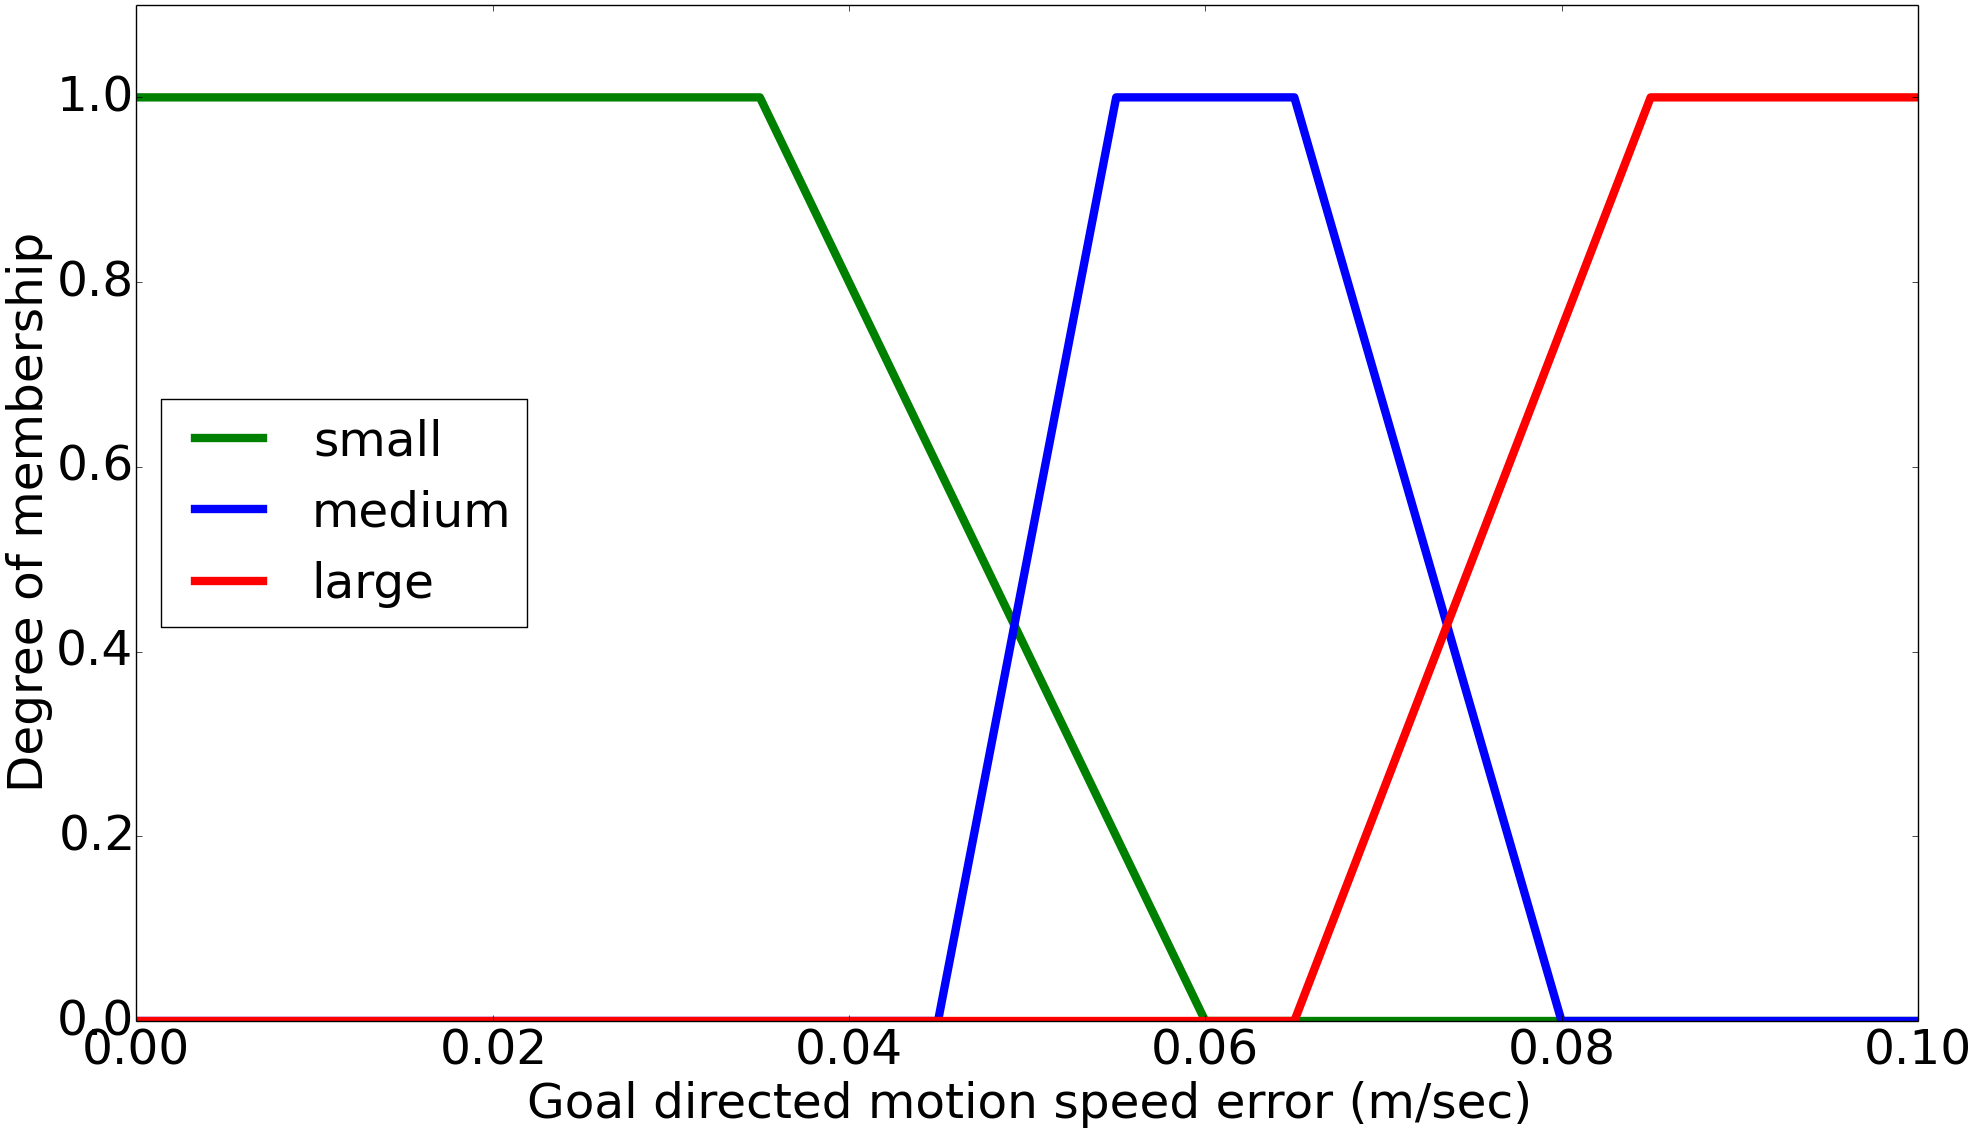
\includegraphics[width=\textwidth]{chapter5_fig/fuzzy_error.png}
			\caption{}
			\label{subfig:fuzzy_error}
		\end{subfigure}
		\hfill
		\begin{subfigure}[b]{0.49\textwidth}
			\centering
			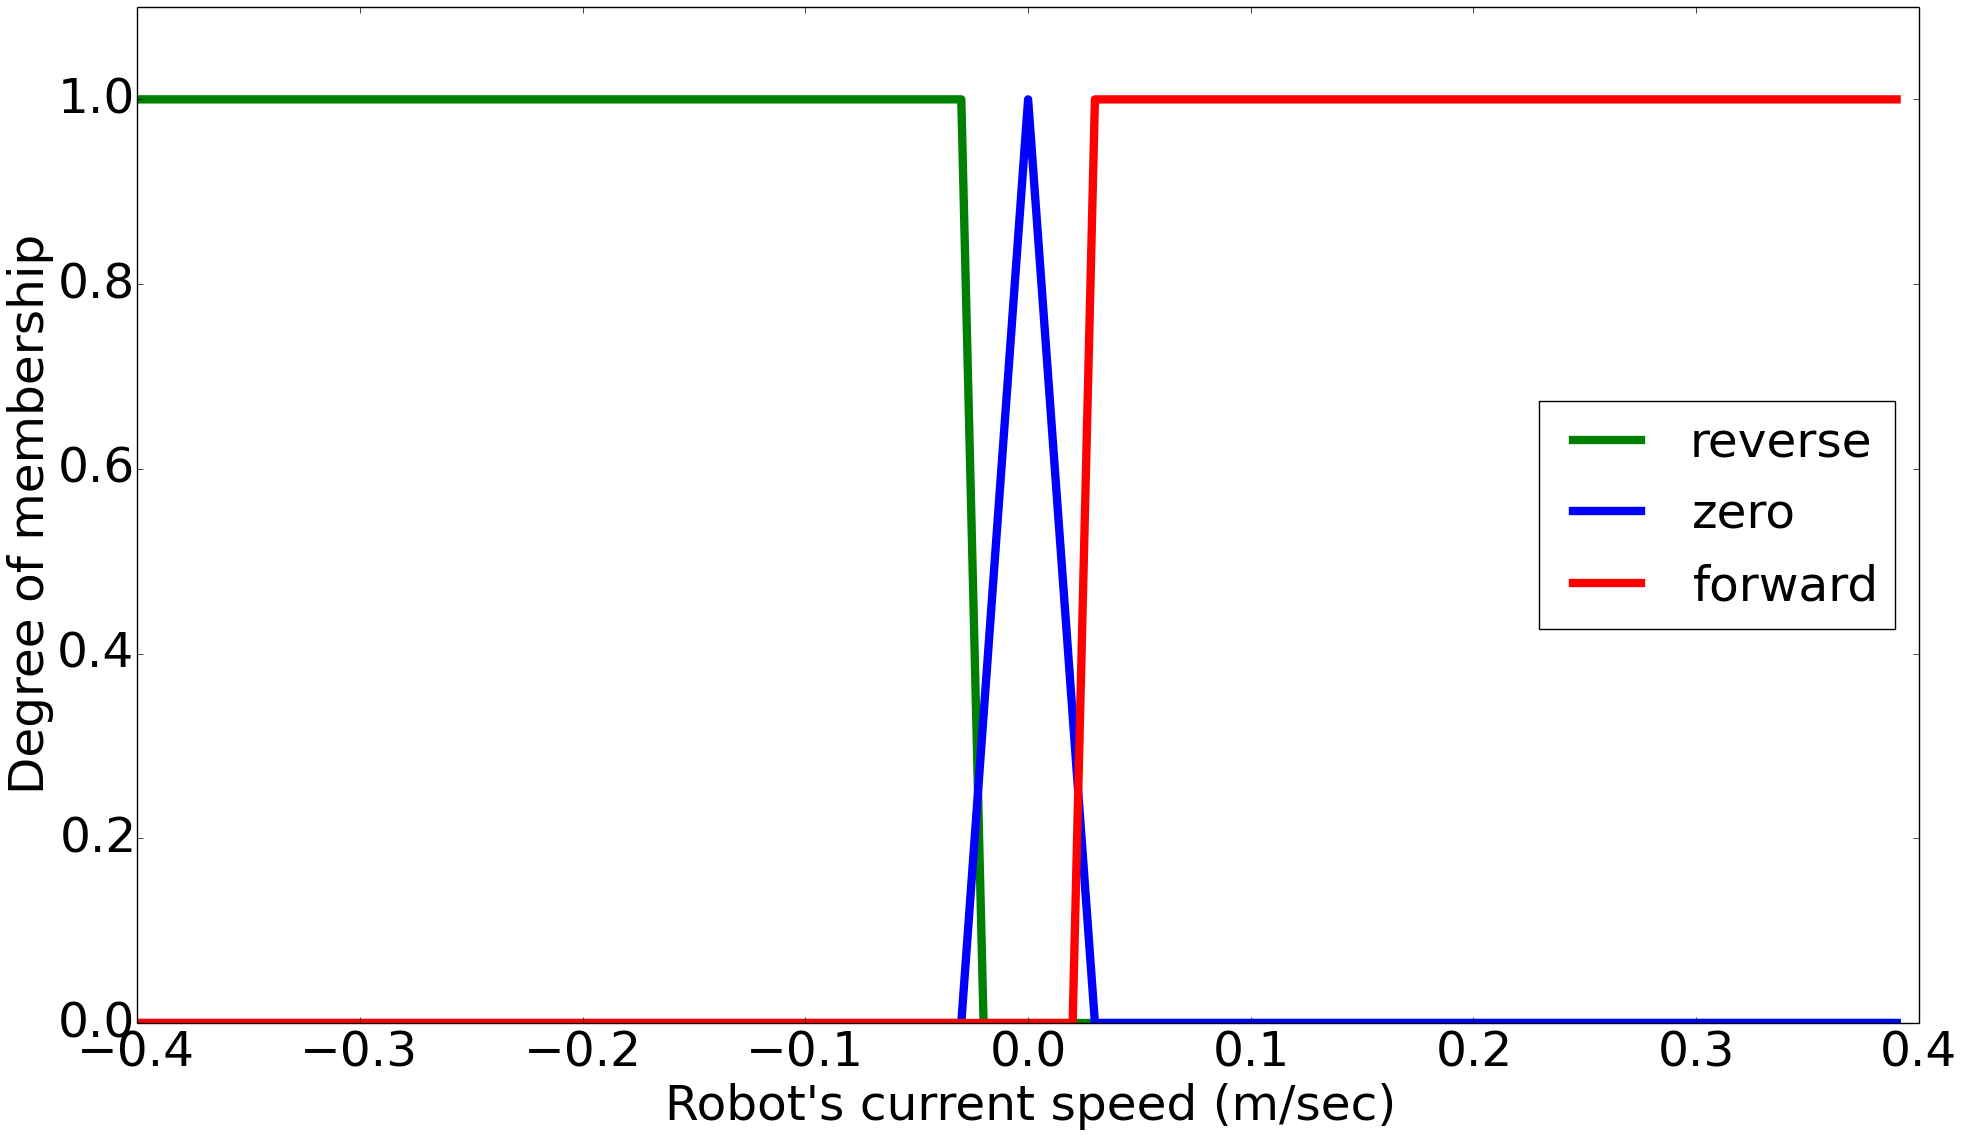
\includegraphics[width=\textwidth]{chapter5_fig/fuzzy_speed.png}
			\caption{}
			\label{subfig:fuzzy_speed}
		\end{subfigure}
		\hfill
		\caption{\textbf{\ref{subfig:fuzzy_error}:} Membership functions for the linguistic input variable "error". \textbf{\ref{subfig:fuzzy_speed}:} Membership functions for linguistic input variable "speed".}
		\label{fig:fuzzy_input}
\end{figure}

For the linguistic input variable $x_1 = "error"$ the universe of discourse (i.e. the range of all possible values for an input) is $X_1 =[0,0.1] m/sec$. A value of $0 m/sec$ means that no goal directed motion error exists, i.e. the robot is doing progress towards the goal without any performance degradation. The value of $0.1 m/sec$ is the maximum error, meaning that the robot is not progressing towards the goal (e.g. robot is idle). This is despite the maximum speed of the robot being $0.4 m/sec$. Due to physical and mechanical constrains (e.g. acceleration limits) the maximum new speed that can be given to the robot at any time, cannot have a difference with the current speed more than $0.1 m/sec$. For the linguistic input variable $x_2 = "speed"$ the universe of discourse is $X_2 = [-0.4,0.4] m/sec$. The value of $0.4 m/sec$ is the maximum speed of the robot. The value of $-0.4 m/sec$ is the maximum reverse speed of the robot. 

The input variable "error" (i.e. $x_1$) is mapped into three linguistic values (i.e. three fuzzy set membership functions, see Fig. \ref{subfig:fuzzy_error}). The set $A_1^i$ for input $x_1$ can be defined for the following linguistic values: $A_1^i = [A_1^1 = small, A_1^2 = medium, A_1^3 = large]$. The error threshold calculated in our previous threshold controller was used to denote the fuzzy linguistic value "large". In essence what operators consider to be a large error to justify a LOA switch, is encoded into the fuzzy controller. This knowledge was extracted by using a grid search algorithm on HI data as described in Section \ref{chapter5:threshold_controller}). The values and membership functions for "small" and "medium" were heuristically chosen in order to smoothly overlap throughout the universe of discourse (see Table \ref{table:membership_functions}). This is a common practice when designing fuzzy controllers. 

The input variable "speed" (i.e. $x_2$) is mapped into three linguistic values (see Fig. \ref{subfig:fuzzy_speed}).The set $A_2^i$ for input $x_2$ can be defined for the following linguistic values: $A_2^i = [A_2^1 = reverse, A_1^2 = zero, A_1^3 = forward]$. The value "reverse" denotes that the robot's speed is negative, which means the robot is reversing. The value "zero" denotes that the robot is idle and not moving. The value "forward" denotes that the robot is moving forward (see Table \ref{table:membership_functions}).

The fuzzyfication process transforms the crisp values of the inputs into fuzzy values. This is achieved using the fuzzy membership functions described above and in Table \ref{table:membership_functions}. Then, a set of fuzzy rules is applied to the fuzzy inputs (see Table \ref{table:rule_base}). The following standard (i.e. commonly used) operators are used in the fuzzy inference process: for conjunction (i.e. "and") the minimum operator is used; for disjunction (i.e. "or") the maximum operator is used; for rule activation the minimum operator is used; for fuzzy rules aggregation the maximum operator is used. The fuzzy rules (see table \ref{table:rule_base}) used in the controller were constructed using expert knowledge from HI data. In essence the fuzzy rules dictate that the controller will initiate a LOA switch only when the "error" is "large" and the robot is not reversing. If the "error" is "large" and the robot is reversing, the assumption is that the agent in control is trying to unstuck the robot. Hence, by taking into account this simplified context knowledge, the controller will not switch LOA.

\begin{figure}
	\centering
	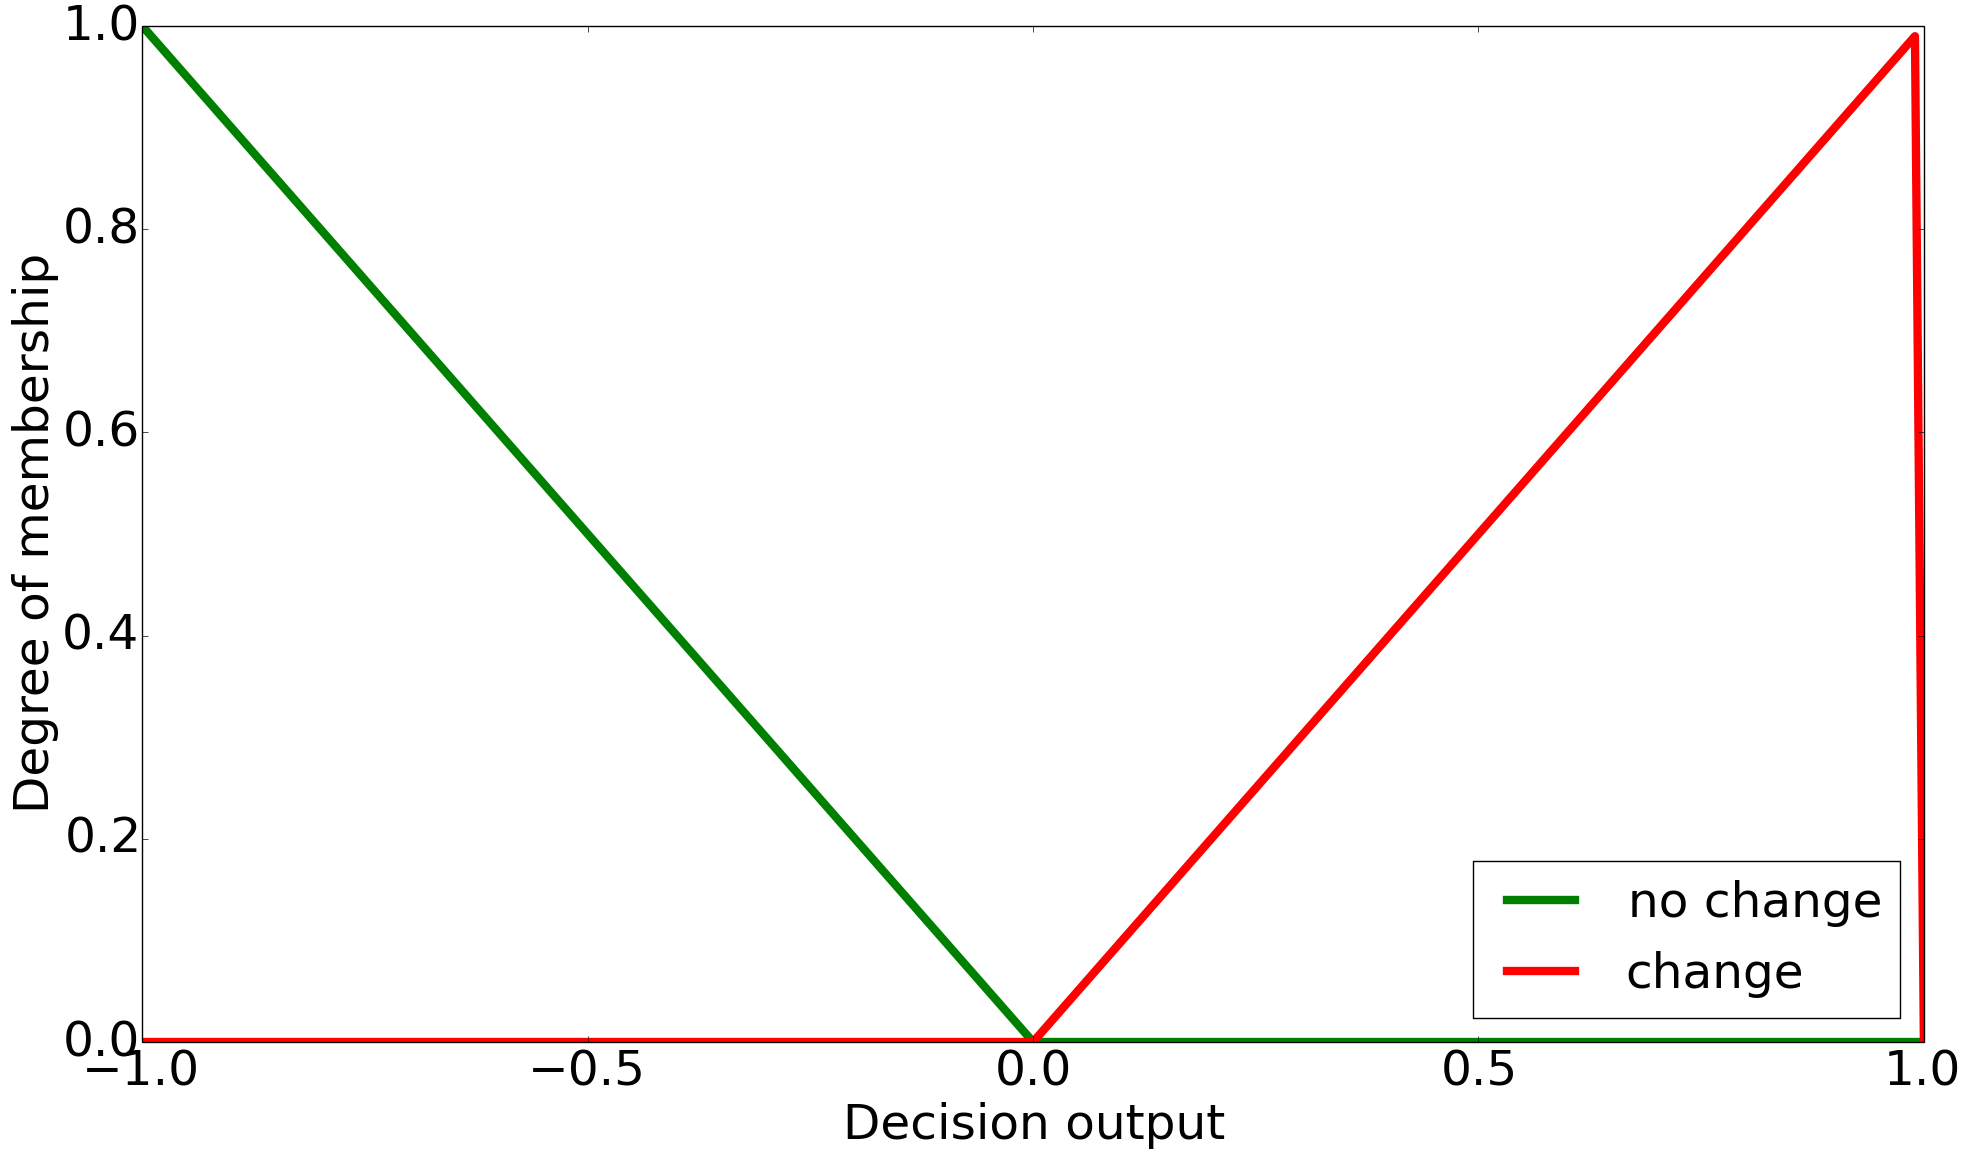
\includegraphics[width=0.6\columnwidth]{chapter5_fig/fuzzy_output.png}
	\caption{Output membership functions.} 
	\label{fig:fuzzy_output}
\end{figure}

Similar to the work of Nagi et al. \citep{Nagi2009} we follow the fuzzy bang-bang relay controller (FBBRC) approach. This means that the Largest of Maxima (LOM) defuzzification method is used. The LOM method has the advantage of directly producing a two-level state output which in our case is mapped into "change" (i.e. switch) LOA and "no change" (see Fig. \ref{fig:fuzzy_output}). This allows for the antecedent part of the fuzzy rules to be freely chosen while the consequent part has only two linguistic values (i.e. "change" or "no change" LOA). The output's universe of discourse $Y = [-1,1]$ represents the bang-bang output. The value of y = -1 means that no LOA switching initiative will take place. The value of $y = 1$ means that the controller will initiate a LOA switch.

The LOA switching problem under investigation is complex, ill-defined, and its underlying dynamics are not precisely known. Thus, a fuzzy controller offers several advantages. Primarily it allows the efficient management of the real world fuzziness, by the use of expert knowledge coming from human operators. This can be easily achieved by extending the fuzzy sets and fuzzy rules base to include new linguistic input variables, metrics, heuristics etc. Potentially, this can also lead to a controller which is to some extend context aware. Additionally, the controller can be extended to have more output states in order to facilitate a more complex system. This is based on the fact that fuzzy logic allows for smoother transition between states. Lastly, fuzzy logic enables more transparency and better understanding of how the controller works, something important given the current state of the research.


\begin{table}
    \begin{tabular}{|c|c|}
    \hline
    No. & Rules                                                                \\ \hline
    1   & \textbf{IF} error is small \textbf{OR} error is medium \textbf{THEN} LOA is no change \\ \hline
    2   & \textbf{IF} error is large \textbf{AND} speed is not reverse \textbf{THEN} LOA is change \\ \hline
    3   & \textbf{IF} speed is reverse \textbf{AND} error is large \textbf{THEN} LOA is no change  \\ \hline
    \end{tabular}
    \caption {The fuzzy rule base.}
    \label{table:rule_base}
\end{table}


 \begin{table}
     \begin{tabular}{|c|c|}
    
     \hline
     Linguistic value & Membership functions       \\ \hline
    
     error small   & $ \mu_{A_1^1}(x_1) = \begin{cases}
     0,  &  0.06 \leq x\\
     1  &  0  \leq x \leq 0.035  \\
     \frac{0.06-x}{0.06-0.035}  &  0.035  \leq x \leq 0.06
     \end{cases} $ \\ \hline
    
     error medium   & $ \mu_{A_1^2}(x_1) = \begin{cases}
     0,  & x \leq  0.045, 0.08 \leq x\\
     \frac{x-0.045}{0.055-0.045}  &  0.045  \leq x \leq 0.055 \\
     1  &  0.055  \leq x \leq 0.065  \\
     \frac{0.08-x}{0.08-0.065}  &  0.065  \leq x \leq 0.08
     \end{cases} $ \\ \hline
  
     error large   & $ \mu_{A_1^3}(x_1) = \begin{cases}
     0,  & x \leq  0.065 \\
     \frac{x-0.065}{b-0.065}  &  0.065  \leq x \leq 0.085 \\
     1  &  0.085  \leq x \leq 0.1  \\
     \end{cases} $ \\ \hline
    
     speed reverse   & $ \mu_{A_2^1}(x_2) = \begin{cases}
     0,  & -0.02 \leq  x \\
     1  &  x \leq -0.03  \\
     \frac{-0.02-x}{-0.02-(-0.03)}  &  -0.03  \leq x \leq -0.02
     \end{cases} $ \\ \hline
    
     speed zero   & $ \mu_{A_2^2}(x_2) = \begin{cases}
     0,  & x \leq  -0.03, 0.03 \leq x\\
     \frac{x-(-0.03)}{0-(-0.03)}  &  -0.03  \leq x \leq 0 \\
     \frac{0.03-x}{0.03}  &  0 \leq x \leq 0.03
     \end{cases} $ \\ \hline
  
     speed forward   & $ \mu_{A_2^3}(x_2) = \begin{cases}
     0,  & 0.02 \leq  x \\
     \frac{x-0.02}{0.03-0.02}  &  0.02  \leq x \leq 0.03 \\
     1  &  0.03  \leq x   \\
     \end{cases} $ \\ \hline
    

     \end{tabular}
     \caption {The fuzzy membership functions for linguistic values of input variables "error" and "speed" (see Fig. \ref{fig:fuzzy_input}). For "error", trapezoid membership functions have been used. For "speed" membership functions, two trapezoid for "reverse" and "forward" and one triangular for "zero", were used. The values and membership functions were heuristically chosen in order to smoothly overlap throughout the universe of discourse. This is a common practice when designing fuzzy controllers. The membership function for "error large" was chosen based on the error threshold calculated in Section \ref{chapter5:threshold_controller}.}
     \label{table:membership_functions}
 \end{table}

\section{Evaluation using a simulated robot and test environment}
\label{chapter5:experiment2_2}

It is important to validate the MI controller using the same framework as before to allow us to make direct comparisons between MI and HI. To be useful, the MI algorithm should provide the same level of performance or better, in terms of primary task completion time or score, as compared to the HI system. The reason that the MI controller can be useful despite potentially having the same level of performance with the HI, is that there are situations in which a human initiated LOA switch may not be possible (e.g. loss of communication or incapacitated operator).


An experimental evaluation of the fuzzy logic MI controller described above was conducted. The aim was to make an initial evaluation of the MI controller and compare it's performance with those of the HI controller. If performance on the tasks prove to be in a similar level or better than the HI controller, then the MI controller has a positive and meaningful impact upon the system. This will be especially true compared to using only teleoperation or autonomy. More specifically the experiment described in this section evaluates: a) the human's and robot's initiatives, especially when they coexist in MI, to switch LOA between teleoperation and autonomy in order to overcome circumstances in which the system is under-performing; b) how the MI controller performs compared to the HI one of Chapter \ref{chapter4:HI}; c) the unfolding Human-Robot Interaction (HRI) of MI control. 

In the previous chapter (see Chapter \ref{chapter4:HI}) we carried out experiments in a high fidelity simulated maze-like test arena (see Fig. \ref{subfig:arena_exp2} and \ref{subfig:map_exp2}) using Human-Initiative (HI) control. The robot was controlled by an Operator Control Unit (OCU), composed of a laptop, a joystick, a mouse and a screen showing the control interface. We used a simulated Pioneer-3DX mobile robot fitted with a camera and a laser scanner. We conducted the experiment described in this section using an identical setup to Chapter \ref{chapter4:HI}, i.e. identical robot arena; system; experimental paradigm and procedures. This is in order to facilitate meaningful comparison between the controllers. The only difference in the system was the addition of Robot-Initiative and Mixed-Initiative control. The \textbf{Mixed-Initiative (MI)} controller, as described in Section \ref{chapter5:designing_MI_nav}, gives the robot and the operator the capacity and authority to switch dynamically (i.e. during task execution) between teleoperation and autonomy. The fuzzy robot controller initiates LOA switches based on \textit{goal directed motion} performance (i.e. effectiveness) and simplified (i.e. limited) context. The operator switches LOA using a button on the joy-pad, according to his/her judgment. The \textbf{Robot-Initiative (RI)} controller uses identical mechanisms with the MI controller for the robot LOA switching behavior. However, it deprives the operator from the LOA switching initiative and thus it restricts him in using the robot's dictated LOA. In both controllers, when a LOA switch occurs, the robot alerts operators in three different ways using: a) an alarm sound identical to the one denoting "engine failure" in airplanes; b) synthetic speech expressing the LOA the robot has switched to; c) a GUI notification.

The 24 participants of our previous HI study were asked to participate in this experiment. From these, 16 volunteered to participate. This allowed us, along with the identical setup, to compare directly the results from MI and RI with the ones of the same participants from the previous experiment. We used a within-groups experimental design with every participant performing two trials: a) one using the MI controller; b) one using the RI controller. Each participant underwent extensive training before the experiment, similar to our previous work, but adapted to the new controllers. This ensured that all participants had adequate understanding of the new system and had attained a common minimum skill level. Counterbalancing was used in the experimental trials (i.e. the order of the tested controllers was rotated for different participants) in order to prevent both learning and fatigue effects from biasing the results. For the mental rotation of 3D objects secondary task, identically to the previous experiment, different cards but of equal difficulty \citep{Ganis2015} were randomized and used in each trial. 

 
\subsection{Results: tasks performance}
\label{chapter5:sim_results_system}
Similar to our previous experiments, statistical analysis was conducted on a number of metrics. A repeated measures one-way ANOVA was used to compare RI, MI and HI. An ANOVA with Greenhouse-Geisser correction was used for the cases that shericity assumption (i.e. that the variances of the differences between trials are not equal) was violated. For the HI, the subset of the data corresponding to the 16 participants was used. Fisher's least significant difference (LSD) test was used for pairwise comparisons. As in previous analyses, we consider a result to be significant when it yields a $p$ value less than $0.05$. Lastly we report on the statistical power of the results and the effect size.

% PRIMARY TIME
ANOVA for \textit{primary task completion time} (see Fig. \ref{subfig:primary_time_score_exp2_2}) showed overall significantly different means (\textit{$F(2, 30) = 19.116$,  $p < .01$, $power = 1$, $\eta^2 = .56$}) between HI variable-autonomy (\textit{$M = 418.5$ $sec$, $SD = 34.9$}), RI (\textit{$M = 392.3$ $sec$, $SD = 22.4$}) and MI (\textit{$M = 374.2$ $sec$, $SD = 15.6$}). Pairwise comparison revealed that HI performed significantly worse (i.e. slower completion time) than the other two control modes with \textit{$p <.01$}. Also MI variable autonomy performed significantly better than RI (\textit{$p <.01$}). 

% COLLISIONS
The effect of control mode on the number of \textit{collisions} was not significant (\textit{$F(1.469, 22.036) = 1$, $p > .05$, $power < 0.8$, $\eta^2 = .062$}) between RI (\textit{$M = .81$, $SD = 1.5$}), MI (\textit{$M = 0.38$, $SD = 0.6$}), and HI variable autonomy mode (\textit{$M = .63$, $SD = 1.1$}).

	\begin{figure}
		\centering
		\begin{subfigure}[b]{0.47\textwidth}
			\centering
			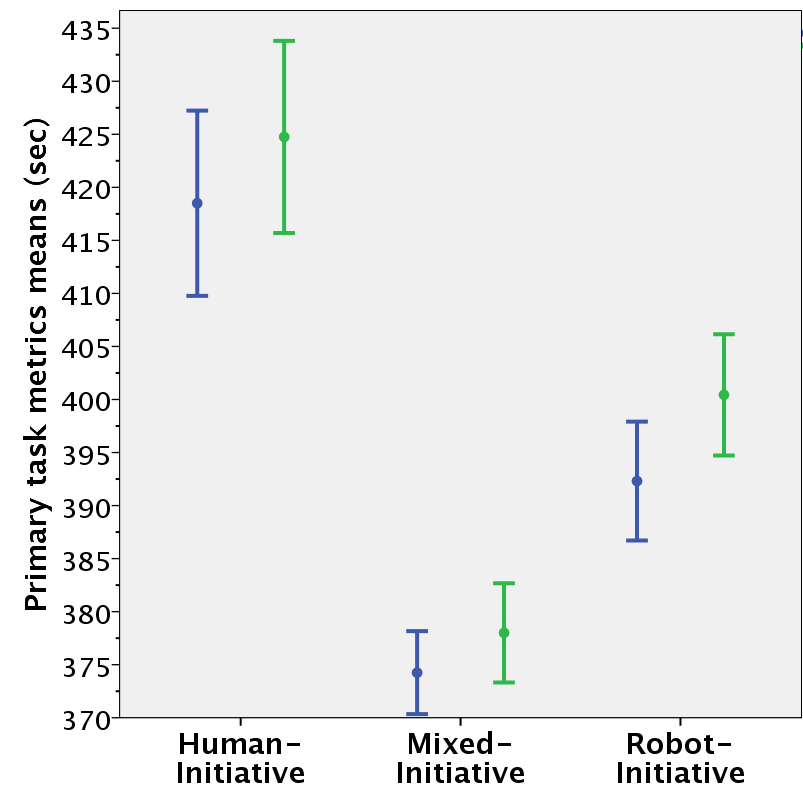
\includegraphics[width=\textwidth]{chapter5_fig/exp2_2_primary_metrics.png}
			\caption{}
			\label{subfig:primary_time_score_exp2_2}
		\end{subfigure}
		\hfill
		\begin{subfigure}[b]{0.5\textwidth}
			\centering
			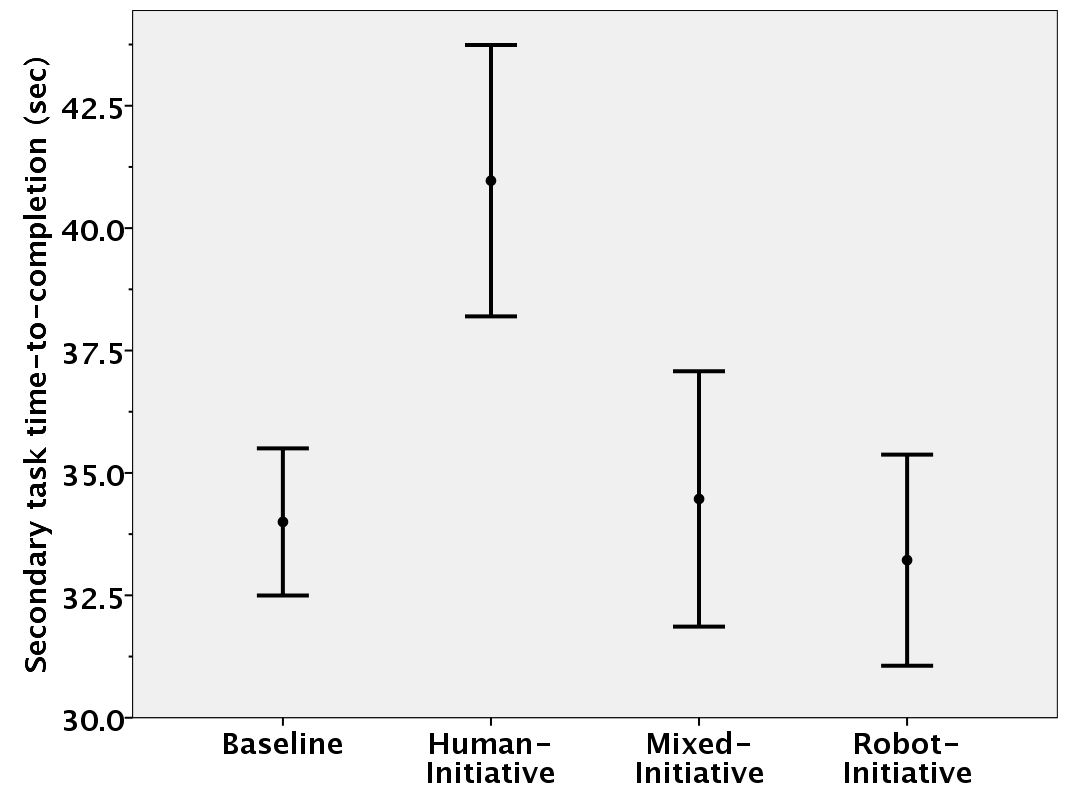
\includegraphics[width=\textwidth]{chapter5_fig/exp2_2_secondary_time.png}
			\caption{}
			\label{subfig:secondarytime_exp2_2}
		\end{subfigure}
		\hfill
		\caption{\textbf{\ref{subfig:primary_time_score_exp2_2}:} primary task results; average time to completion (blue) and score (green) combining time and collisions penalty. \textbf{\ref{subfig:secondarytime_exp2_2}:} secondary task time-to-completion. In all graphs the error bars indicate the standard error.}
		\label{fig:primary_secondary_exp2_2}
	\end{figure}

% PRIMARY SCORE
As in previous chapters, we used the \textit{primary task score} in order to be able to capture the speed-accuracy trade-off that different operators might have (i.e. how fast an operator is driving the robot vs how carefully). The primary task score (see Fig. \ref{subfig:primary_time_score_exp2_2}) is calculated by adding a time penalty of \textit{$10$ $sec$} for every collision, onto the primary task completion time for each participant. ANOVA analysis showed that control mode had a significant effect on primary task score (\textit{$F(2, 30) = 16.774$, $p < .01$, $power > 0.9$, $\eta^2 = .528$}). LSD test suggests that HI variable autonomy (\textit{$M = 424.8$, , $SD = 36.2$}) is significantly (\textit{$p <.01$}) worse than the MI mode (\textit{$M = 378$, $SD = 18.7$}) and the RI mode ( \textit{$M = 400.4$, $SD = 22.9$, $p =.01$}). Lastly MI significantly (\textit{$p <.01$}) outperformed RI regarding primary task score. 

% SECONDARY TIME
The average time per trial that the participants took to complete one series of the 3D object rotations, is denoted by the \textit{Secondary task completion time} (see Fig. \ref{subfig:secondarytime_exp2_2}). ANOVA (\textit{$F(3, 45) = 10.344, p < .01 , power > .95$, , $\eta^2 = .408$}) showed that there is a significant difference between the means of secondary task completion times. HI variable autonomy mode (\textit{$M = 40$ $sec$, $SD = 11.1$}) performed significantly worse (i.e. more time to complete) than the other modes with $p < .01$. Performance between the baseline trial (\textit{$M = 34$ $sec$, $SD = 6$}), the MI mode (\textit{$M = 34.5$ $sec$, $SD = 10.4$}) and RI mode (\textit{$M = 33.2$ $sec$, $SD = 8.6$}) were without any significant difference ($p > .05$, i.e. same level of performance).

% SECONDARY MISTAKES
The \textit{number of secondary task errors} (see Fig. \ref{subfig:psecondary_mistakes_exp2_2}) is the average number of mistake/errors per trial that the participants did during one series of the 3D object rotations. The number of secondary task errors did not had significant differences between the different control modes as showed by ANOVA  (\textit{$F(3, 45) = 0.891, p > .05 , power < .8$, $\eta^2 = .056$}). Participants had \textit{$M = 1.7$ ($SD = 1.7$)} errors during baseline tests (i.e. without operating the robot); \textit{$M = 1.7$ ($SD = 1.67$)} during HI variable autonomy mode; \textit{$M = 2$ ($SD = 1.67$)} in RI mode; and \textit{$M = 1.4$ ($SD = 1.4$)} in MI mode.

	\begin{figure}
		\centering
		\begin{subfigure}[b]{0.48\textwidth}
			\centering
			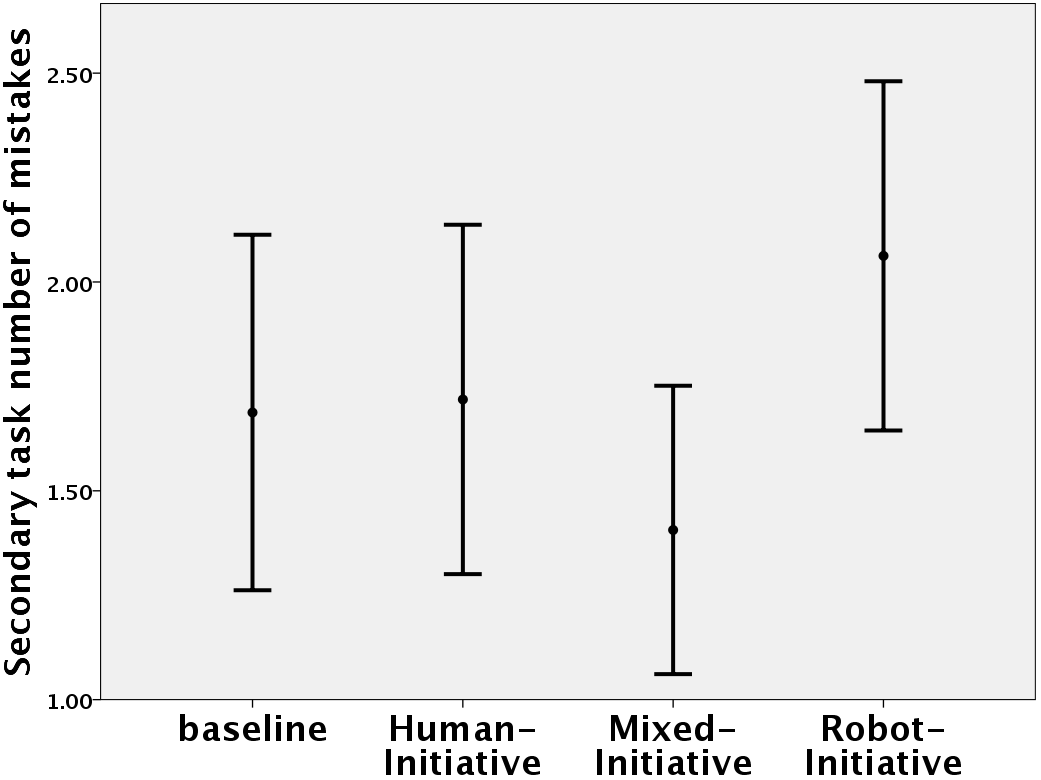
\includegraphics[width=\textwidth]{chapter5_fig/exp2_2_secondary_mistakes.png}
			\caption{}
			\label{subfig:psecondary_mistakes_exp2_2}
		\end{subfigure}
		\hfill
		\begin{subfigure}[b]{0.48\textwidth}
			\centering
			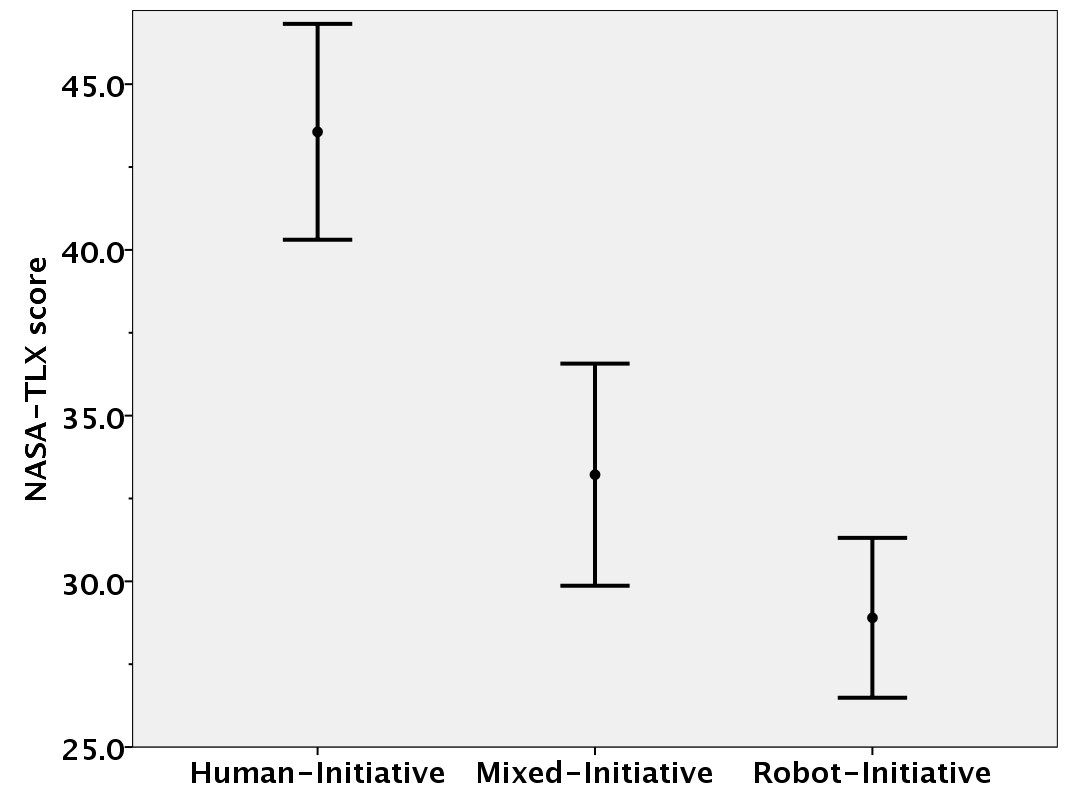
\includegraphics[width=\textwidth]{chapter5_fig/exp2_2_NASA-TLX.png}
			\caption{}
			\label{subfig:NASA-TLX_exp2_2}
		\end{subfigure}
		\hfill
		\caption{ \textbf{\ref{subfig:psecondary_mistakes_exp2_2}:} secondary task average number of mistakes/errors. \textbf{\ref{subfig:NASA-TLX_exp2_2}:} NASA-TLX score showing the overall trial difficulty/workload as perceived by the operators.}
		\label{fig:nasa_secondary_exp2_2}
	\end{figure}
    

% NASA-TLX
Control mode had a significant effect on \textit{NASA-TLX scores} (see Fig. \ref{subfig:NASA-TLX_exp2_2}) as showed by ANOVA (\textit{$F(1.337, 20.049) = 10.135, p < .01 , power > .9$, $\eta^2 = .403$}). Pairwise comparisons showed that RI (\textit{$M = 28.899$, $SD = 9.642$}) was perceived by participants as having the lowest difficulty, as compared to HI variable autonomy mode (\textit{$M = 43.561$, $SD = 13.026$}) with $p < 0.01$ and MI mode (\textit{$M = 33.217$, $SD = 13.399$}) with $p = 0.05$. HI variable autonomy is perceived as being more difficult than MI ($p < 0.01$). 


\subsection{Results: Human-Robot-Interaction}
\label{chapter5:sim_results_HRI}
% time in mode
Similar to Section \ref{chapter4:results_HRI} we analyzed the average \textit{percentage of time spent in autonomy} for each controller. Due to corrupted data for one of the participants, data from 15 participants was used for every result reported on this particular metric. This is contrary to the rest of the analysis in which data from all 16 participants was used. ANOVA did not showed any effect caused from control mode in the average percentage of time spent in autonomy (\textit{$F(2, 25) = 0.74, p > .05 , power < .8$, $\eta^2 = .50$}). The average percentage of time spent in autonomy for the HI controller was \textit{$M = 57.7\%$} (\textit{$SD = 25.9$}) for the MI controller was \textit{$M = 53\%$} (\textit{$SD = 23.25$}), and for the RI was \textit{$M = 49.1\%$} (\textit{$SD = 12.22$}).

% Number of LOA switches
The \textit{number of LOA switches} (see Fig. \ref{fig:number-loa-switches_exp2_2}) performed in each trial denotes the frequency in which operators made use of the variable autonomy controller capabilities in HI; frequency that operators and AI used the variable autonomy controller in MI; and frequency in which AI used the variable autonomy controllers in RI. ANOVA showed that control mode had a significant effect (\textit{$F(2, 30) = 16.78, p < .01 , power > .9$, $\eta^2 = .528$}) on the number of LOA switches. Pairwise comparisons showed that RI (\textit{$M = 3.13$, $SD = 1.15$}) had significantly ($p < 0.01$) fewer LOA switches as compared to HI mode (\textit{$M = 10.4$, $SD = 8.64$}) and MI mode (\textit{$M = 13.6$, $SD = 11.78$}). The number of LOA switches of HI and MI control modes were on the same level (i.e. no statistical difference, $p > 0.05$). Out of the $13.6$ MI LOA switches, $1.3$ were initiated from the fuzzy MI controller. For completeness we present the histograms illustrating the number of LOA switches in MI and HI (see Fig. \ref{subfig:histogram_lao_hi_exp2_2} and Fig. \ref{fig:histograms_mi_exp2_2}).

	\begin{figure}
		\centering
		\begin{subfigure}[b]{0.49\textwidth}
			\centering
			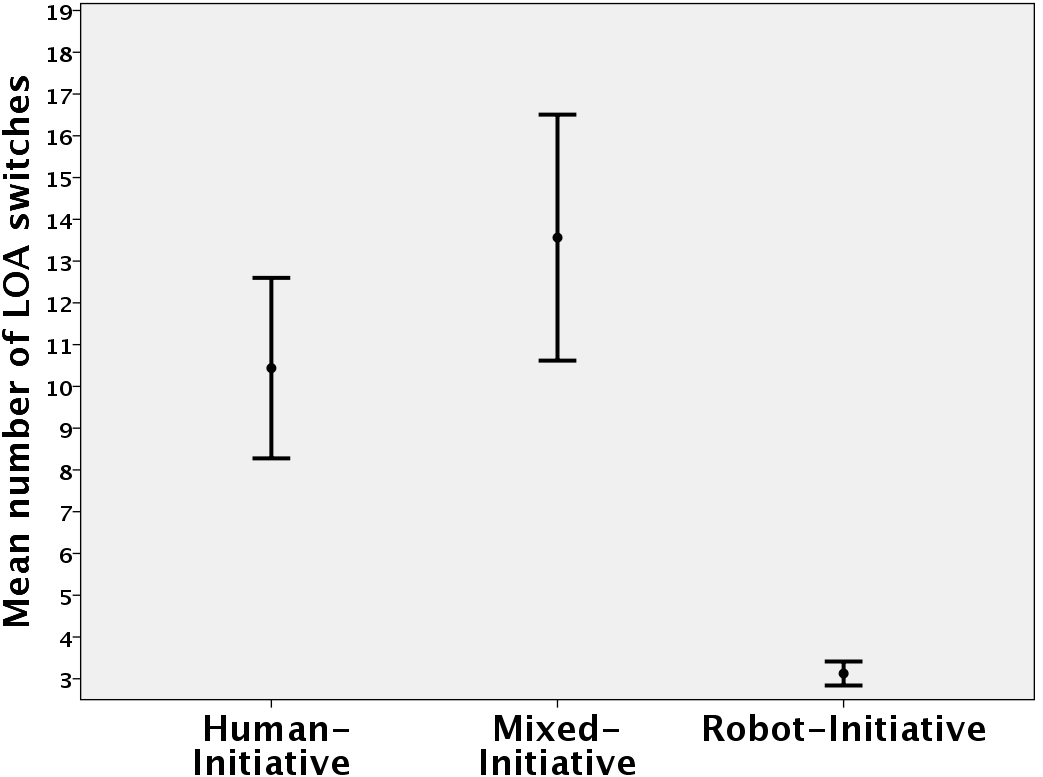
\includegraphics[width=\textwidth]{chapter5_fig/exp2_2_loa_switches.png}
			\caption{}
			\label{fig:number-loa-switches_exp2_2}
		\end{subfigure}
		\hfill
		\begin{subfigure}[b]{0.45\textwidth}
			\centering
			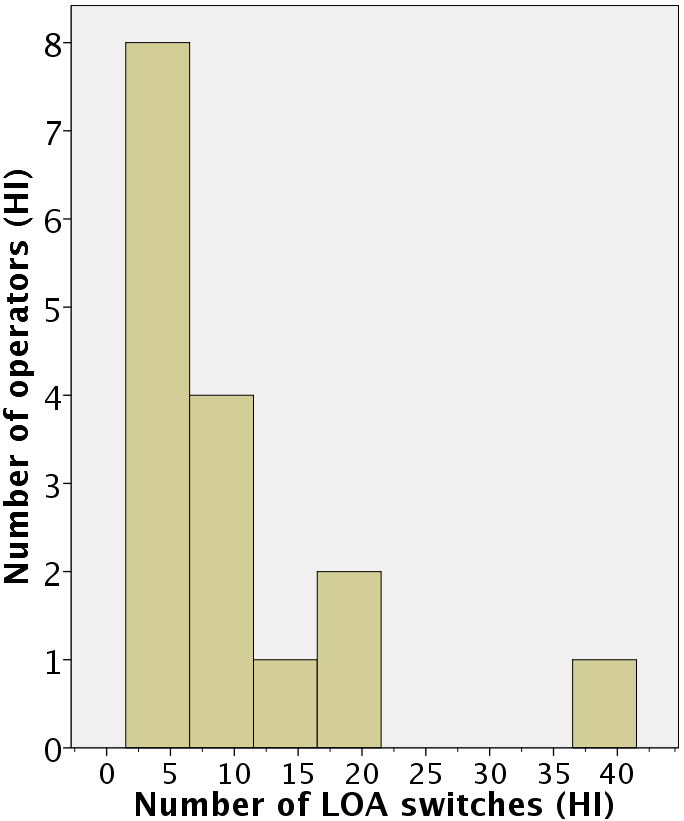
\includegraphics[width=\textwidth]{chapter5_fig/histogram_loa_hi_exp2_2.png}
			\caption{}
			\label{subfig:histogram_lao_hi_exp2_2}
		\end{subfigure}
		\hfill
		\caption{\textbf{\ref{fig:number-loa-switches_exp2_2}:} The average number of LOA switches per control mode. \textbf{\ref{subfig:histogram_lao_hi_exp2_2}:} Histogram showing the number of human operators who chose to make various different numbers of LOA switches during HI.}
		\label{fig:loa_histogram_exp2_2}
	\end{figure}

	\begin{figure}
		\centering
		\begin{subfigure}[b]{0.45\textwidth}
			\centering
			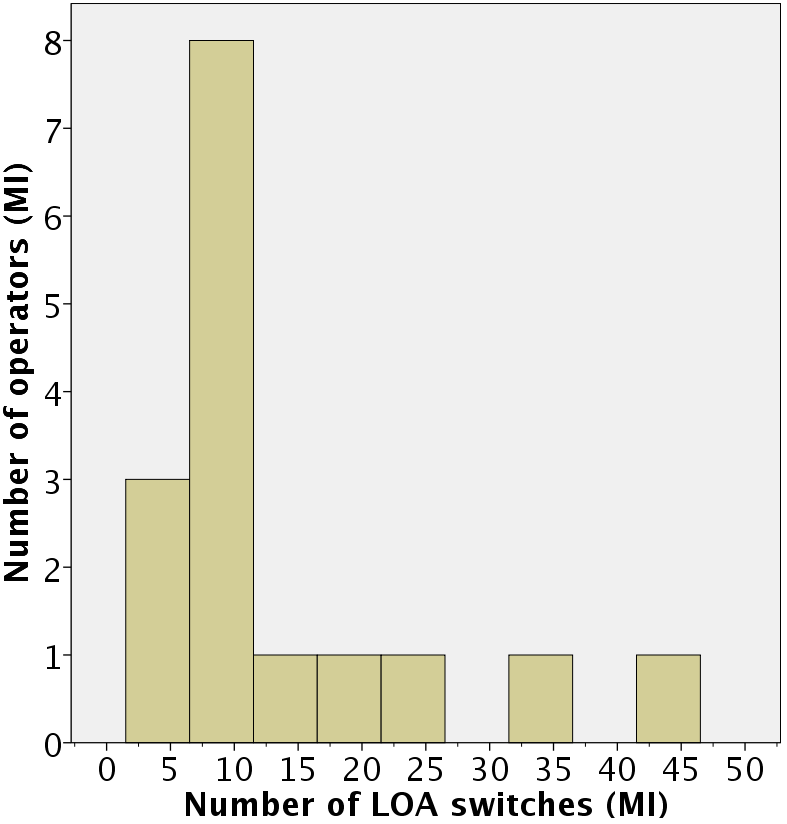
\includegraphics[width=\textwidth]{chapter5_fig/histogram_loa_mi_exp2_2.png}
			\caption{}
			\label{subfig:histogram_lao_mi_exp2_2}
		\end{subfigure}
		\hfill
		\begin{subfigure}[b]{0.45\textwidth}
			\centering
			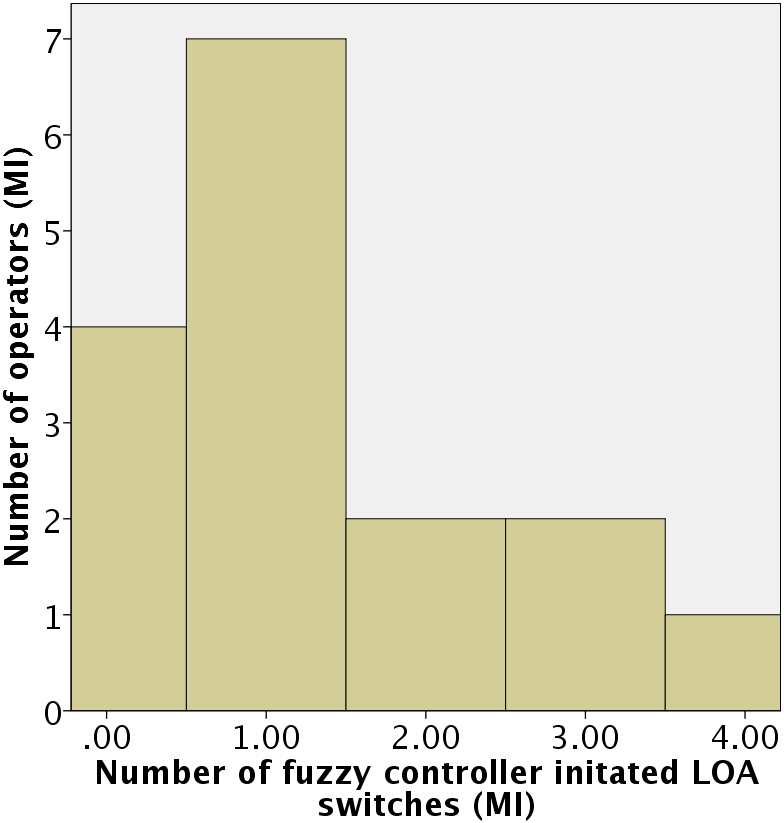
\includegraphics[width=\textwidth]{chapter5_fig/histogram_loa_mi_ai_exp2_2.png}
			\caption{}
			\label{subfig:histogram_lao_mi_ai_exp2_2}
		\end{subfigure}
		\hfill
		\caption{\textbf{\ref{subfig:histogram_lao_mi_exp2_2}:} Histogram showing the number of human operators who chose to make various different numbers of LOA switches during MI. \textbf{\ref{subfig:histogram_lao_mi_ai_exp2_2}:} Histogram showing the number of human operators and the number of LOA switches initiated by the fuzzy MI controller.}
		\label{fig:histograms_mi_exp2_2}
	\end{figure}

% Correlations between LOA switches in different modes
We performed a correlation analysis using a two-tailed Pearson's $r$ to investigate any relationships between different metrics and other variables. The \textit{number of LOA switches} in HI and the \textit{number of LOA switches} in MI are highly correlated ($r(14)= .849, p<.01 $). There was no correlation, similar to HI (see Section \ref{chapter4:results_HRI}), between the \textit{number of LOA switches} and performance in the \textit{primary task score} or \textit{secondary task completion time} in RI and in MI.

% Correlations between time spent in auto in different modes
No correlation was found between the \textit{percentage of time spent in autonomy} in HI and MI ($r(13)= .202, p>.05$); and between the \textit{percentage of time spent in autonomy} in HI and RI ($r(13)= .094, p>.05$). No correlation was found between MI and RI \textit{percentage of time spent in autonomy} ($r(13)= .326, p>.05$).

% Correlations between time spent in auto and primary score
The \textit{percentage of time spent in autonomy} LOA is positively correlated with the \textit{primary task score} in RI ($r(13)= .528, p<.05$). Also the same metrics are positively correlated in MI ($r(13)= .627, p<.05$). As expected given results in Section \ref{chapter4:results_HRI}, no correlation was found between \textit{primary task score} in HI and \textit{percentage of time spent in autonomy} in HI ($r(13)= .047, p>.05$).

% Correlations between time spent in auto and secondary score
Lastly, no correlation was found between \textit{time spent in autonomy} and \textit{secondary task completion time} for none of the 3 control modes, HI (as found in Section \ref{chapter4:results_HRI}), MI, and RI.


\subsection{Discussion}
Mixed-Initiative (MI) and Robot-Initiative (RI) outperformed Human-Initiative (HI) in terms of primary task performance. What this shows primarily, in the context of this experiment, is that the fuzzy robot controller (i.e. both in MI and in RI) is capable of successfully and timely measure performance; infer if a switch in the LOA is needed; and initiate a LOA switch. This is particularly true given that RI performs better than HI, meaning that the fuzzy robot controller initiative is at least as good as operator's judgment in switching LOA (i.e. compared to the HI of Chapter \ref{chapter4:HI}). The fact that MI outperforms RI, possibly indicates learning effects in performing the primary task and the LOA switching. If that is the case, then it is due to the fact that we used the same participants in an identical experimental setup. However, this was necessary for a systematic initial evaluation of the MI controller.

In terms of secondary task performance, MI and RI outperform HI. The secondary task completion time for MI and RI is faster than HI and on the same level of performance as the baseline condition (i.e. secondary task conducted in isolation from the primary task). This can be explained by two possible causes: a) secondary task learning effects; b) the fact that operators were feeling confident to completely neglect the robot and focus on the secondary task, given its capabilities to take initiative and alert the operator. The latter is reinforced by anecdotal evidence as informal chat with the participants revealed that most of them trusted the robot to take control and progress towards the navigation goal if needed. As one of the participants put it "even if I completely neglect the robot, at least it will do something meaningful".

NASA-TLX showed that RI was perceived as marginally easier (i.e. less workload) than MI; and both MI and RI were perceived as significantly easier than HI. This can be an indication of the extra cognitive overhead that operators might have when they need to switch LOA only based on judgment (e.g. HI). It is also an indication that having operators knowing that the robot will help them if needed, makes the task seem as easier. This is particularly true about the RI, as reflected in the NASA-TLX scores. Operators were restricted not to switch LOA themselves and thus, were not concerned about the LOA switching, just complied with AI's initiative. This is in contrast to MI in which operators still had to do some thinking about switching LOA.

There was no statistical difference in the average time spent in autonomy between HI, MI, and RI. Despite that fact, the time spent in autonomy for MI and RI was correlated with the primary task performance, contrary to HI. This possibly has to do with the fact that in MI and RI the time spent in each LOA (i.e. teleoperation and autonomy) was almost equally split. It is an indication that both LOA can equally contribute towards performance depending on the circumstances and the degradation factors.

Regarding the number of LOA switches in MI and HI, not only they were on the same level but they were also highly and positively correlated. The positive correlation means that participants followed similar patterns in the \textit{number of LOA switches} both in HI and in MI. For example, participants that switched LOA very frequently in HI, also switched LOA very frequently in MI and vise versa for low frequency. This reinforces the findings of Chapter \ref{chapter4:HI} that operators not only switch LOA based on reasons beyond performance, but also that personality traits play potentially a big role. Furthermore, the idea that some of the operator's LOA switching is redundant, is further reinforced by the fact LOA switches in RI were much less frequent than HI and MI. 

Lastly, out of the $13.6$ LOA switches in MI, $1.3$ were initiated by the robot. This means that despite operators' proven LOA switching capabilities and learning effects, there are circumstances in which the robot is successfully contributing by taking initiative. However, for some participants (4 out of the 16), the robot did not contribute any LOA switch. This means that the fuzzy MI controller is successful at choosing not to switch LOA when a switch is not needed. Given the variety of operator styles observed (i.e. high frequency and low frequency switches), this is not trivial, and is evidence that the controller is able to cope with different driving styles using the same parameter set.

\section{Evaluation using real robot and test environment}
\label{chapter5:experiment3}
In the previous section an experiment was conducted in simulation in order to perform an initial assessment of the MI controller and the robot's ability to take initiative and switch LOA in a useful manner (e.g. contributing towards better task performance). The initial assessment of our novel MI controller was successful in the sense that both the operators and the robot were able to take initiative (i.e. switch LOA) and produce improved performance compared to HI. This was for both the secondary and the primary tasks. However, part of the improved performance can be possibly explained by learning effects. Moreover, despite the use of a systematic and coherent experimental framework, the experiment took place in simulation. This means that the environment, despite its realism, was well controlled and most of the performance degrading factors were part of the experimental design. This is a very important first step when conducting scientifically repeatable research, however the MI controller lacked proof of generalization. Generalization in this context means that the controller should be able to function well (i.e. similar performance to previous evaluation) in a different setting and under different conditions than the ones that led to its design (e.g. previous simulated environment). More specifically, that the controller will perform well in a new real world environment (e.g. different layout, different obstacles) and under different conditions (e.g. new USAR tasks, different performance degrading factors).

The experiment presented in this section was designed to tackle the limitations described above. This is achieved by conducting a real world experiment with a real robot in a less controlled setting. More specifically the experiment aims to: a) provide evidence that the MI controller can generalize; b) factor out any learning effects that might have affected the results of the previous experiment; c) shift our experimental paradigm towards more complex, realistic environments and tasks.
 

\subsection{Experimental setup - apparatus, robot test arena, and control modes}
In the experiment described here, we used identical software; variable autonomy controllers; interface (see Fig. \ref{subfig:interface_exp3}); and Operator Control Unit (OCU - see Fig. \ref{subfig:OCU_exp3}) to our previous experiments in simulation (see Section \ref{chapter5:experiment2_2} and Chapter \ref{chapter4:HI}). The robot used was the Pioneer-3DX from our previous real world experiment (see Chapter \ref{chapter3:towards}) equipped with a laser range finder and a camera (see Fig. \ref{subfig:pioneer_exp3}). Operators controlled the robot remotely, from a separate location, via the control interface. Any Situation-Awareness (SA) was solely gained from the control interface. The communications link between the robot and the OCU was achieved via WiFi.

\begin{figure}
		\centering
		\begin{subfigure}[b]{0.45\textwidth}
			\centering
			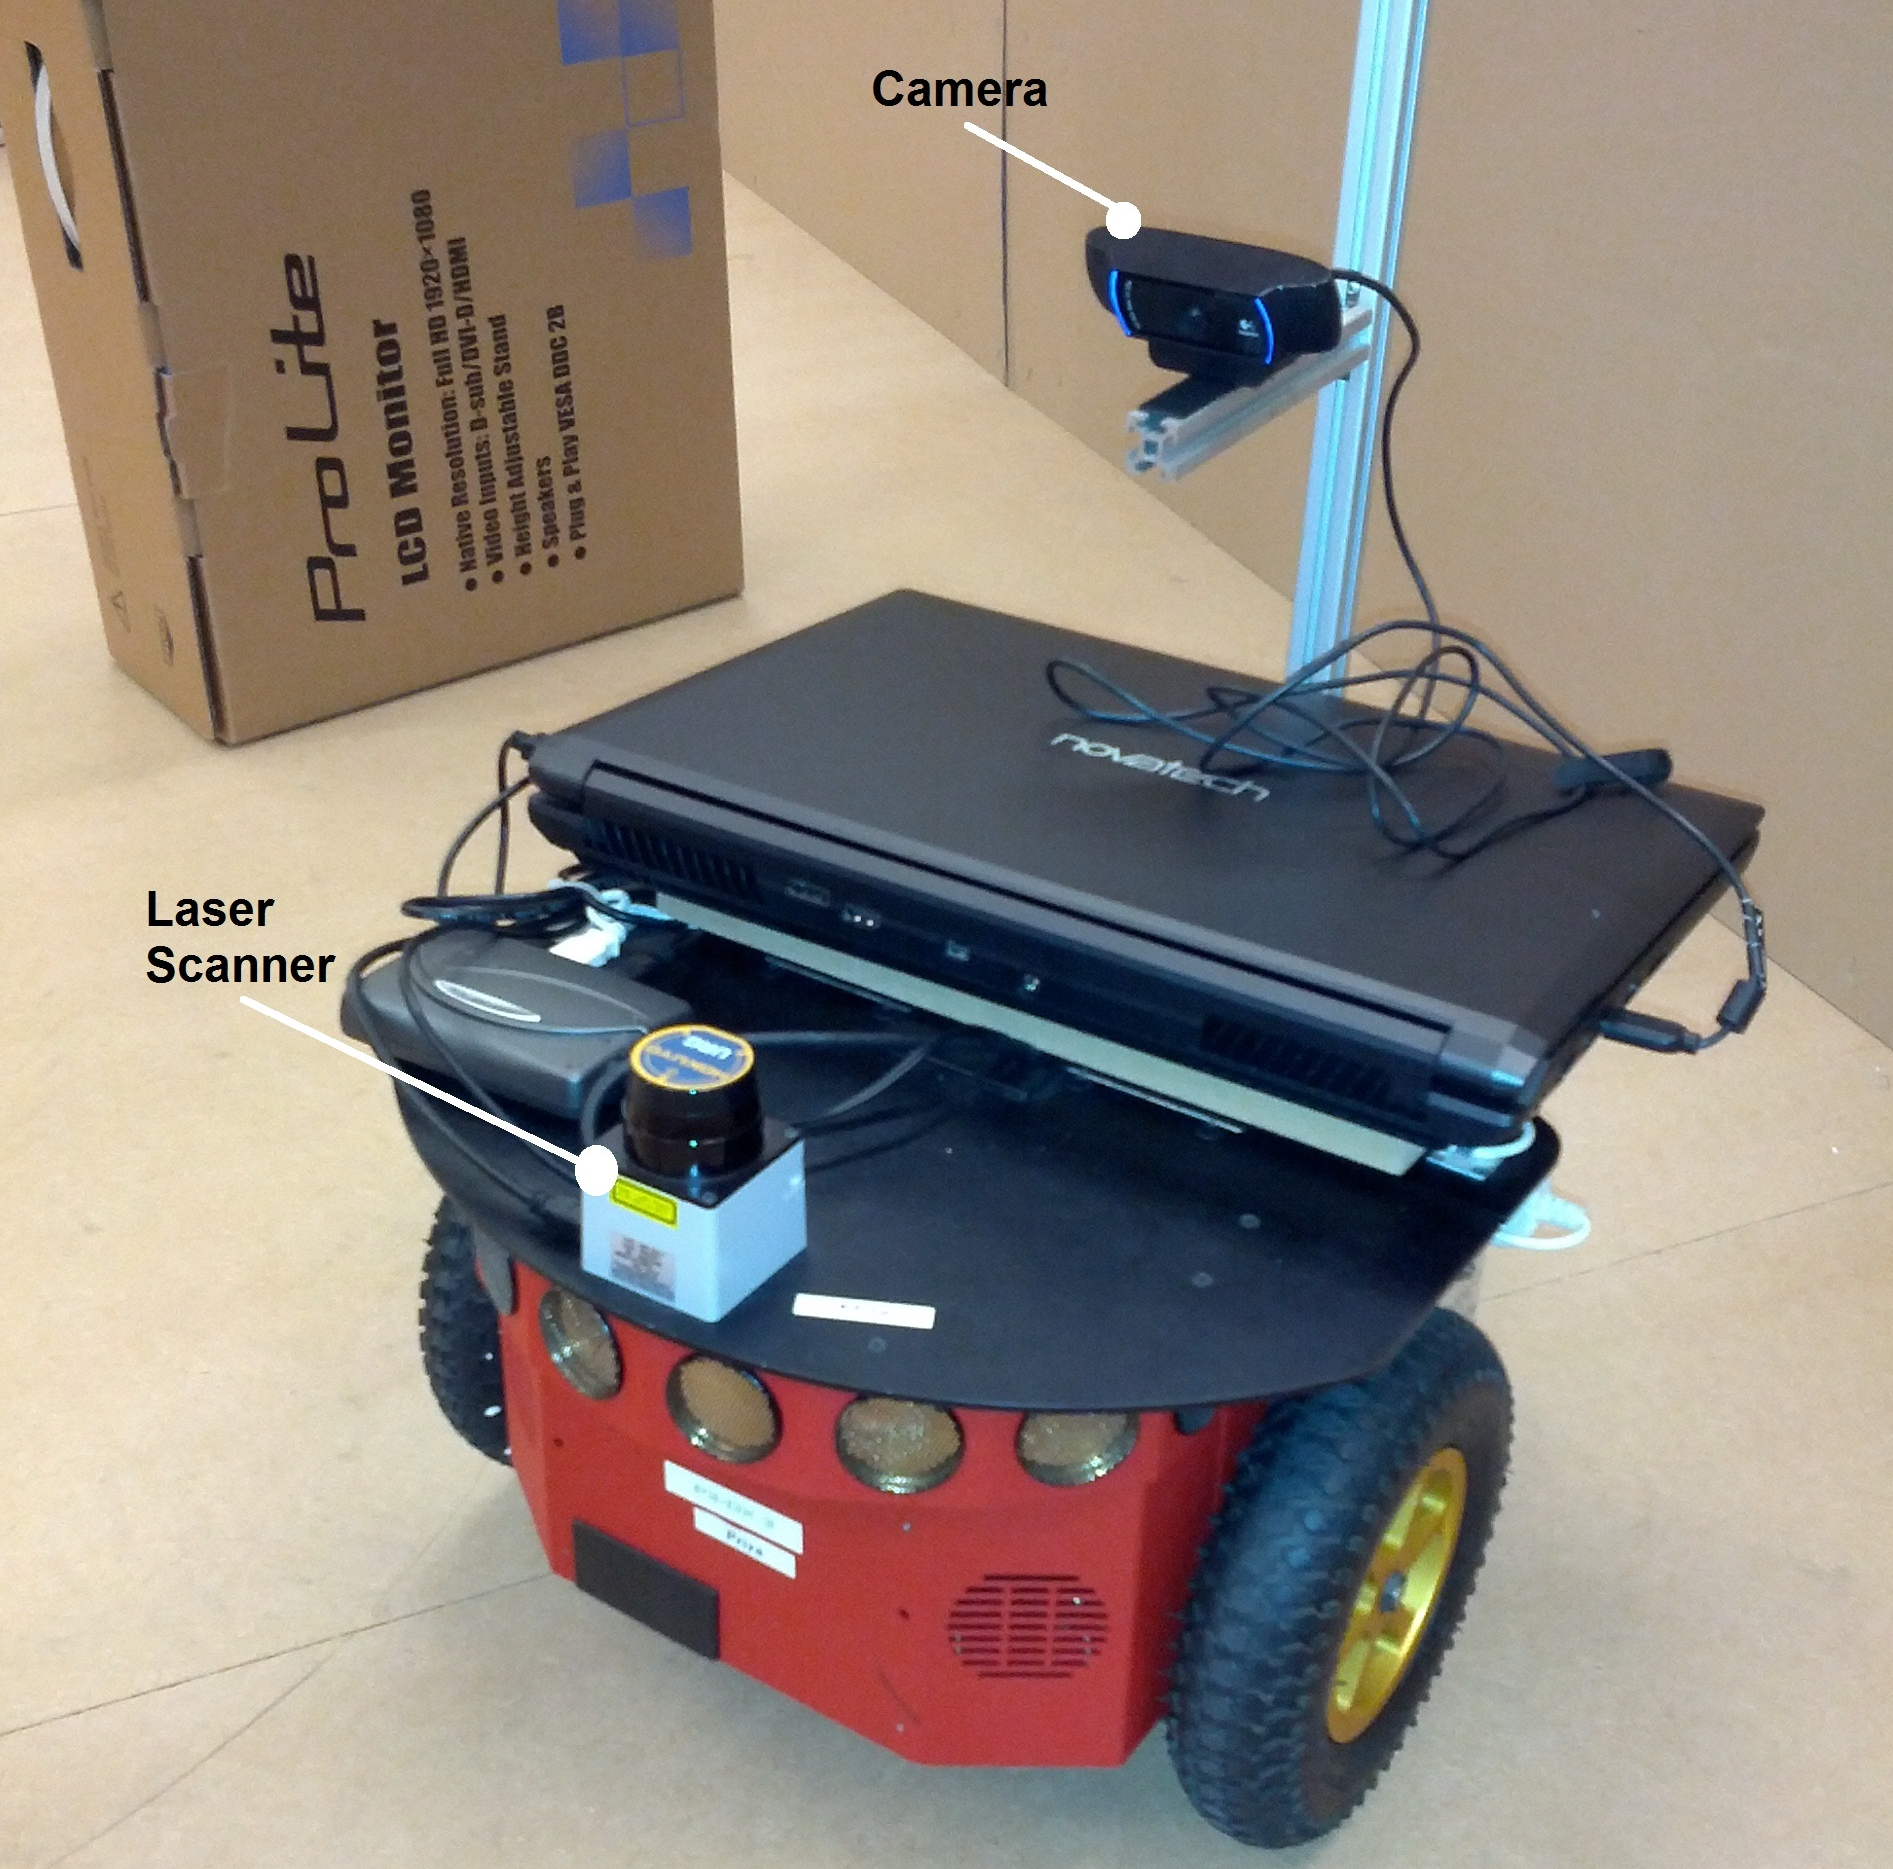
\includegraphics[width=\textwidth]{chapter5_fig/pioneer.jpg}
			\caption{}
			\label{subfig:pioneer_exp3}
		\end{subfigure}
		\hfill
		\begin{subfigure}[b]{0.5\textwidth}
			\centering
			\includegraphics[width=\textwidth]{chapter5_fig/ocu_exp3.jpg}
			\caption{}
			\label{subfig:OCU_exp3}
		\end{subfigure}
		\hfill
		\caption{ \ref{subfig:pioneer_exp3}: The pioneer 3DX robot used in the experiment. \ref{subfig:OCU_exp3}: the Operator Control Unit (OCU), composed of a laptop, a joystick, a mouse and a screen showing the control interface. The same OCU was used in all variable autonomy experiments. Note the floor plan in front of the screen, used for the secondary task.}
		\label{fig:robot_ocu_exp3}
	\end{figure}
      
As in the previous experiments our system offers two LOA: \textbf{Teleoperation:} the human operator drives the robot manually with the joystick. \textbf{Autonomy:} the operator gives high level navigation goals to the robot, by clicking a desired destination on the 2D map. Then the robot autonomously navigates towards this destination. 

Three different control modes were tested in the experiment described here: 1) pure \textbf{teleoperation}, in which the operator was restricted in using only teleoperation LOA; 2) \textbf{Human-Initiative (HI)}, in which the operator could dynamically switch between the teleoperation and autonomy LOA using a button press; 3) \textbf{Mixed-Initiative (MI)}, in which both the operator and the robot had the ability and authority to dynamically switch between autonomy and teleoperation LOA.

\begin{figure}
		\centering
		\begin{subfigure}[b]{0.32\textwidth}
			\centering
			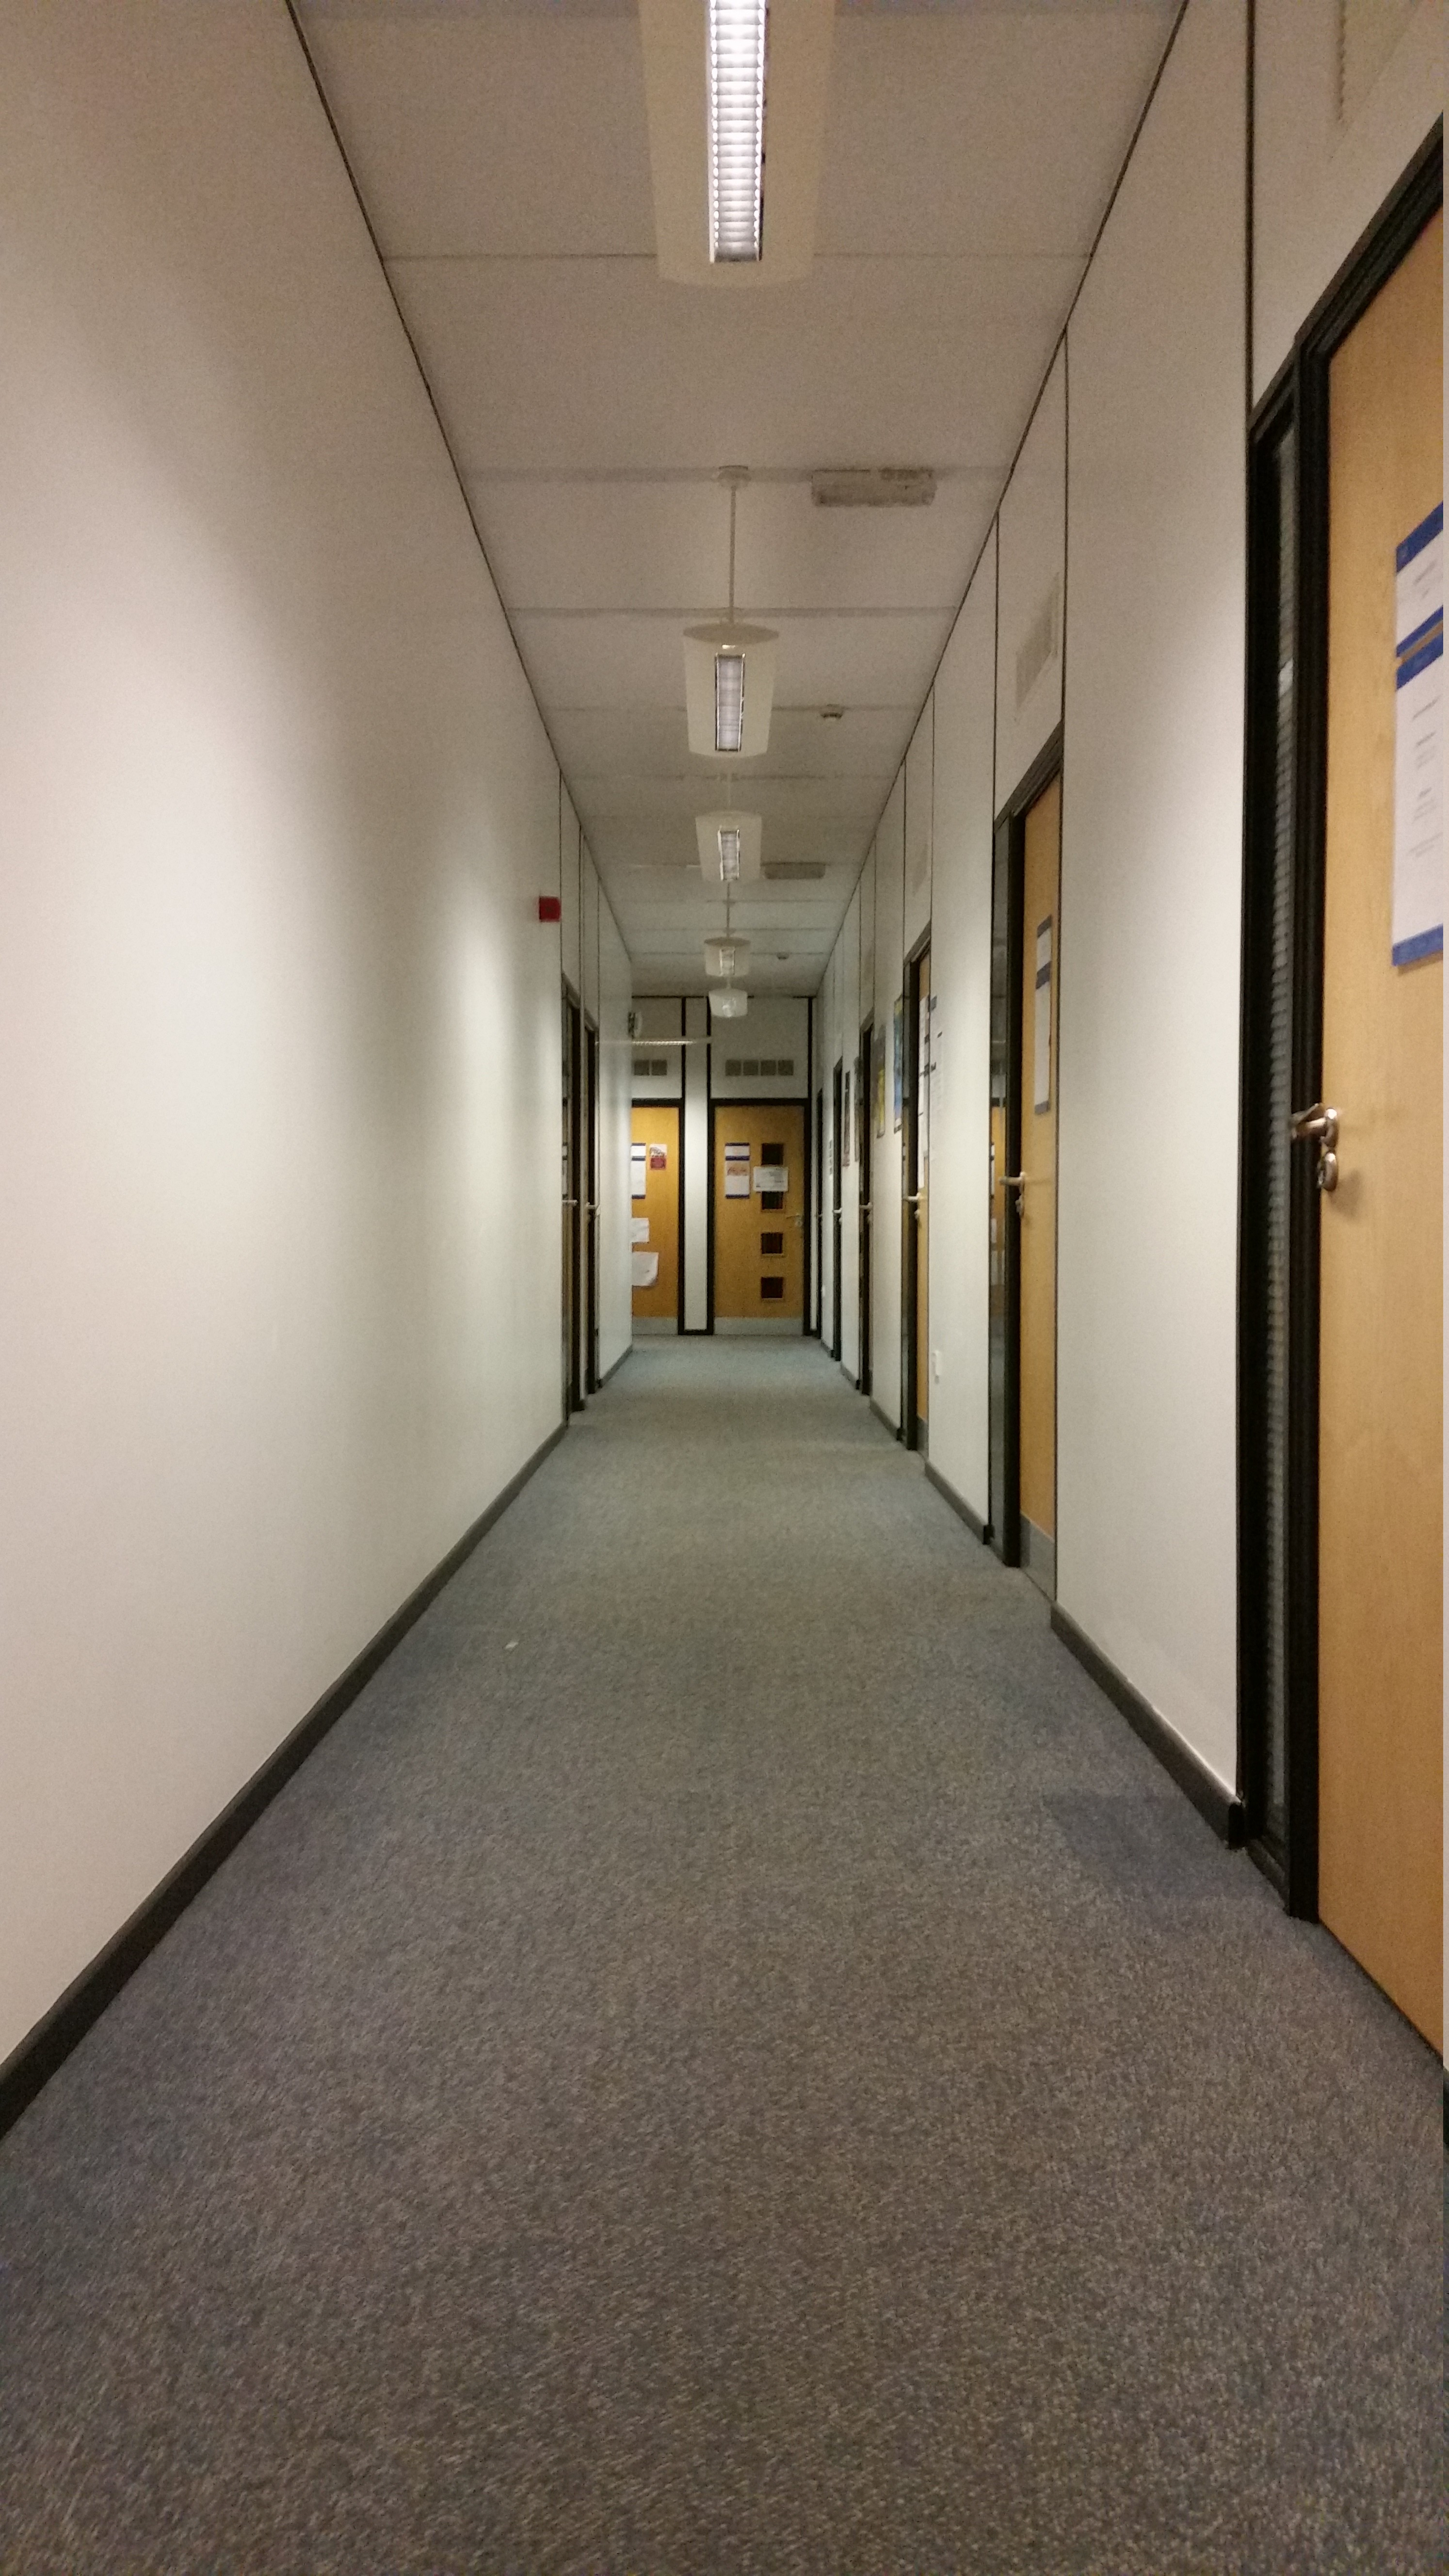
\includegraphics[width=\textwidth]{chapter5_fig/corridor.jpg}
			\caption{}
			\label{subfig:corridor_exp3}
		\end{subfigure}
		\hfill
		\begin{subfigure}[b]{0.65\textwidth}
			\centering
			
\includegraphics[width=\textwidth]{chapter5_fig/office.jpg}
			\caption{}
			\label{subfig:office_exp3}
		\end{subfigure}
		\hfill
		\caption{The first floor of School of Computer Science, University of Birmingham building, was used as a robot arena for the USAR experiment. \textbf{\ref{subfig:corridor_exp3}:} The long corridor that connected the search areas (i.e. offices). \textbf{\ref{subfig:office_exp3}:} One of the offices used as a search area.}
		\label{fig:cs_arena_exp3}
	\end{figure}

Part of the first floor of School of Computer Science, University of Birmingham building, was used as a robot arena for this experiment (see Fig. \ref{subfig:map_exp3} and Fig. \ref{subfig:floorplan}). More specifically, a long corridor (see Fig. \ref{subfig:corridor_exp3}), 2 offices (see Fig. \ref{subfig:office_exp3}) and an open space of approximately $100.7$ square meters in total were used. The experiment took place on weekends and out of hours in order to prevent human activity in the building to be a confounding factor. 

\begin{figure}
		\centering
		\begin{subfigure}[b]{0.4\textwidth}
			\centering
			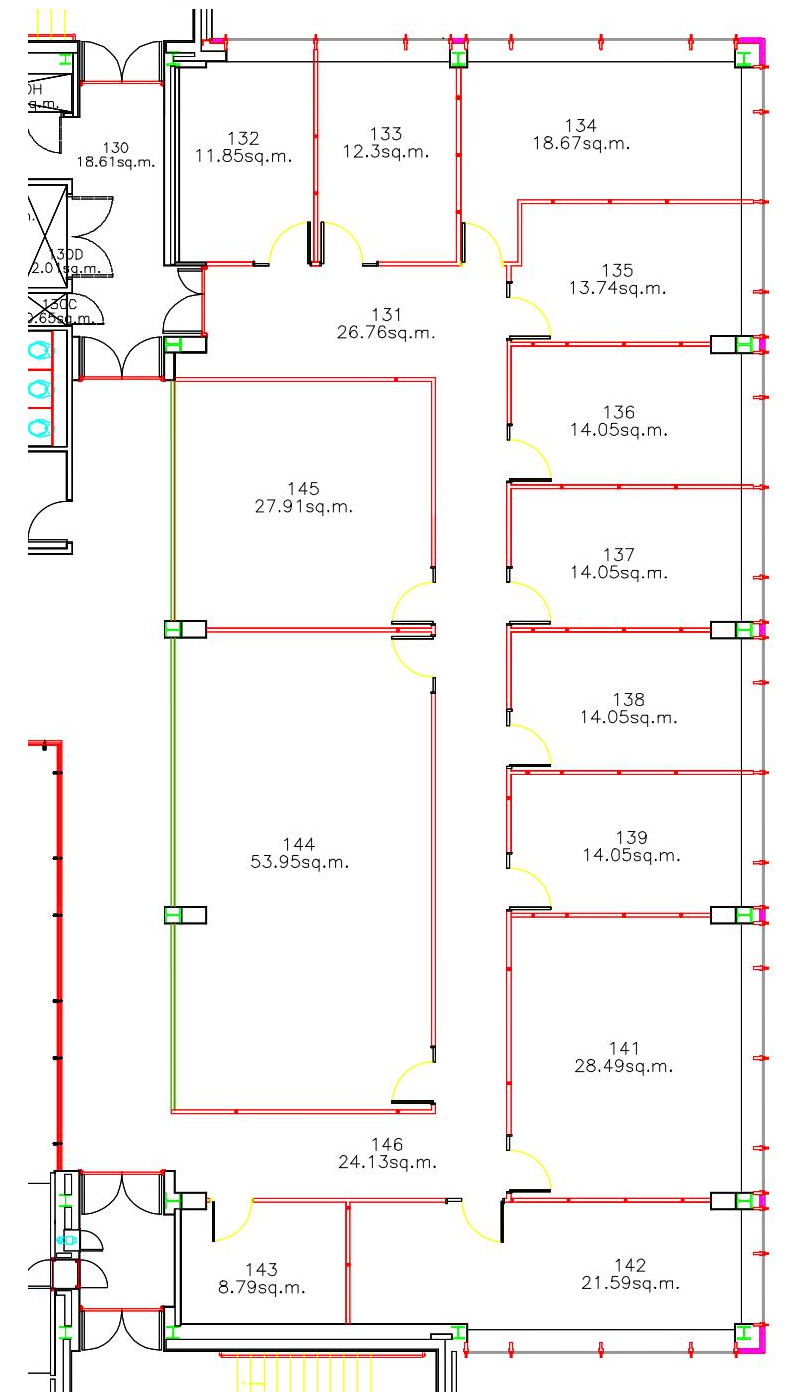
\includegraphics[width=\textwidth]{chapter5_fig/floorplan.png}
			\caption{}
			\label{subfig:floorplan}
		\end{subfigure}
		\hfill
		\begin{subfigure}[b]{0.49\textwidth}
			\centering
			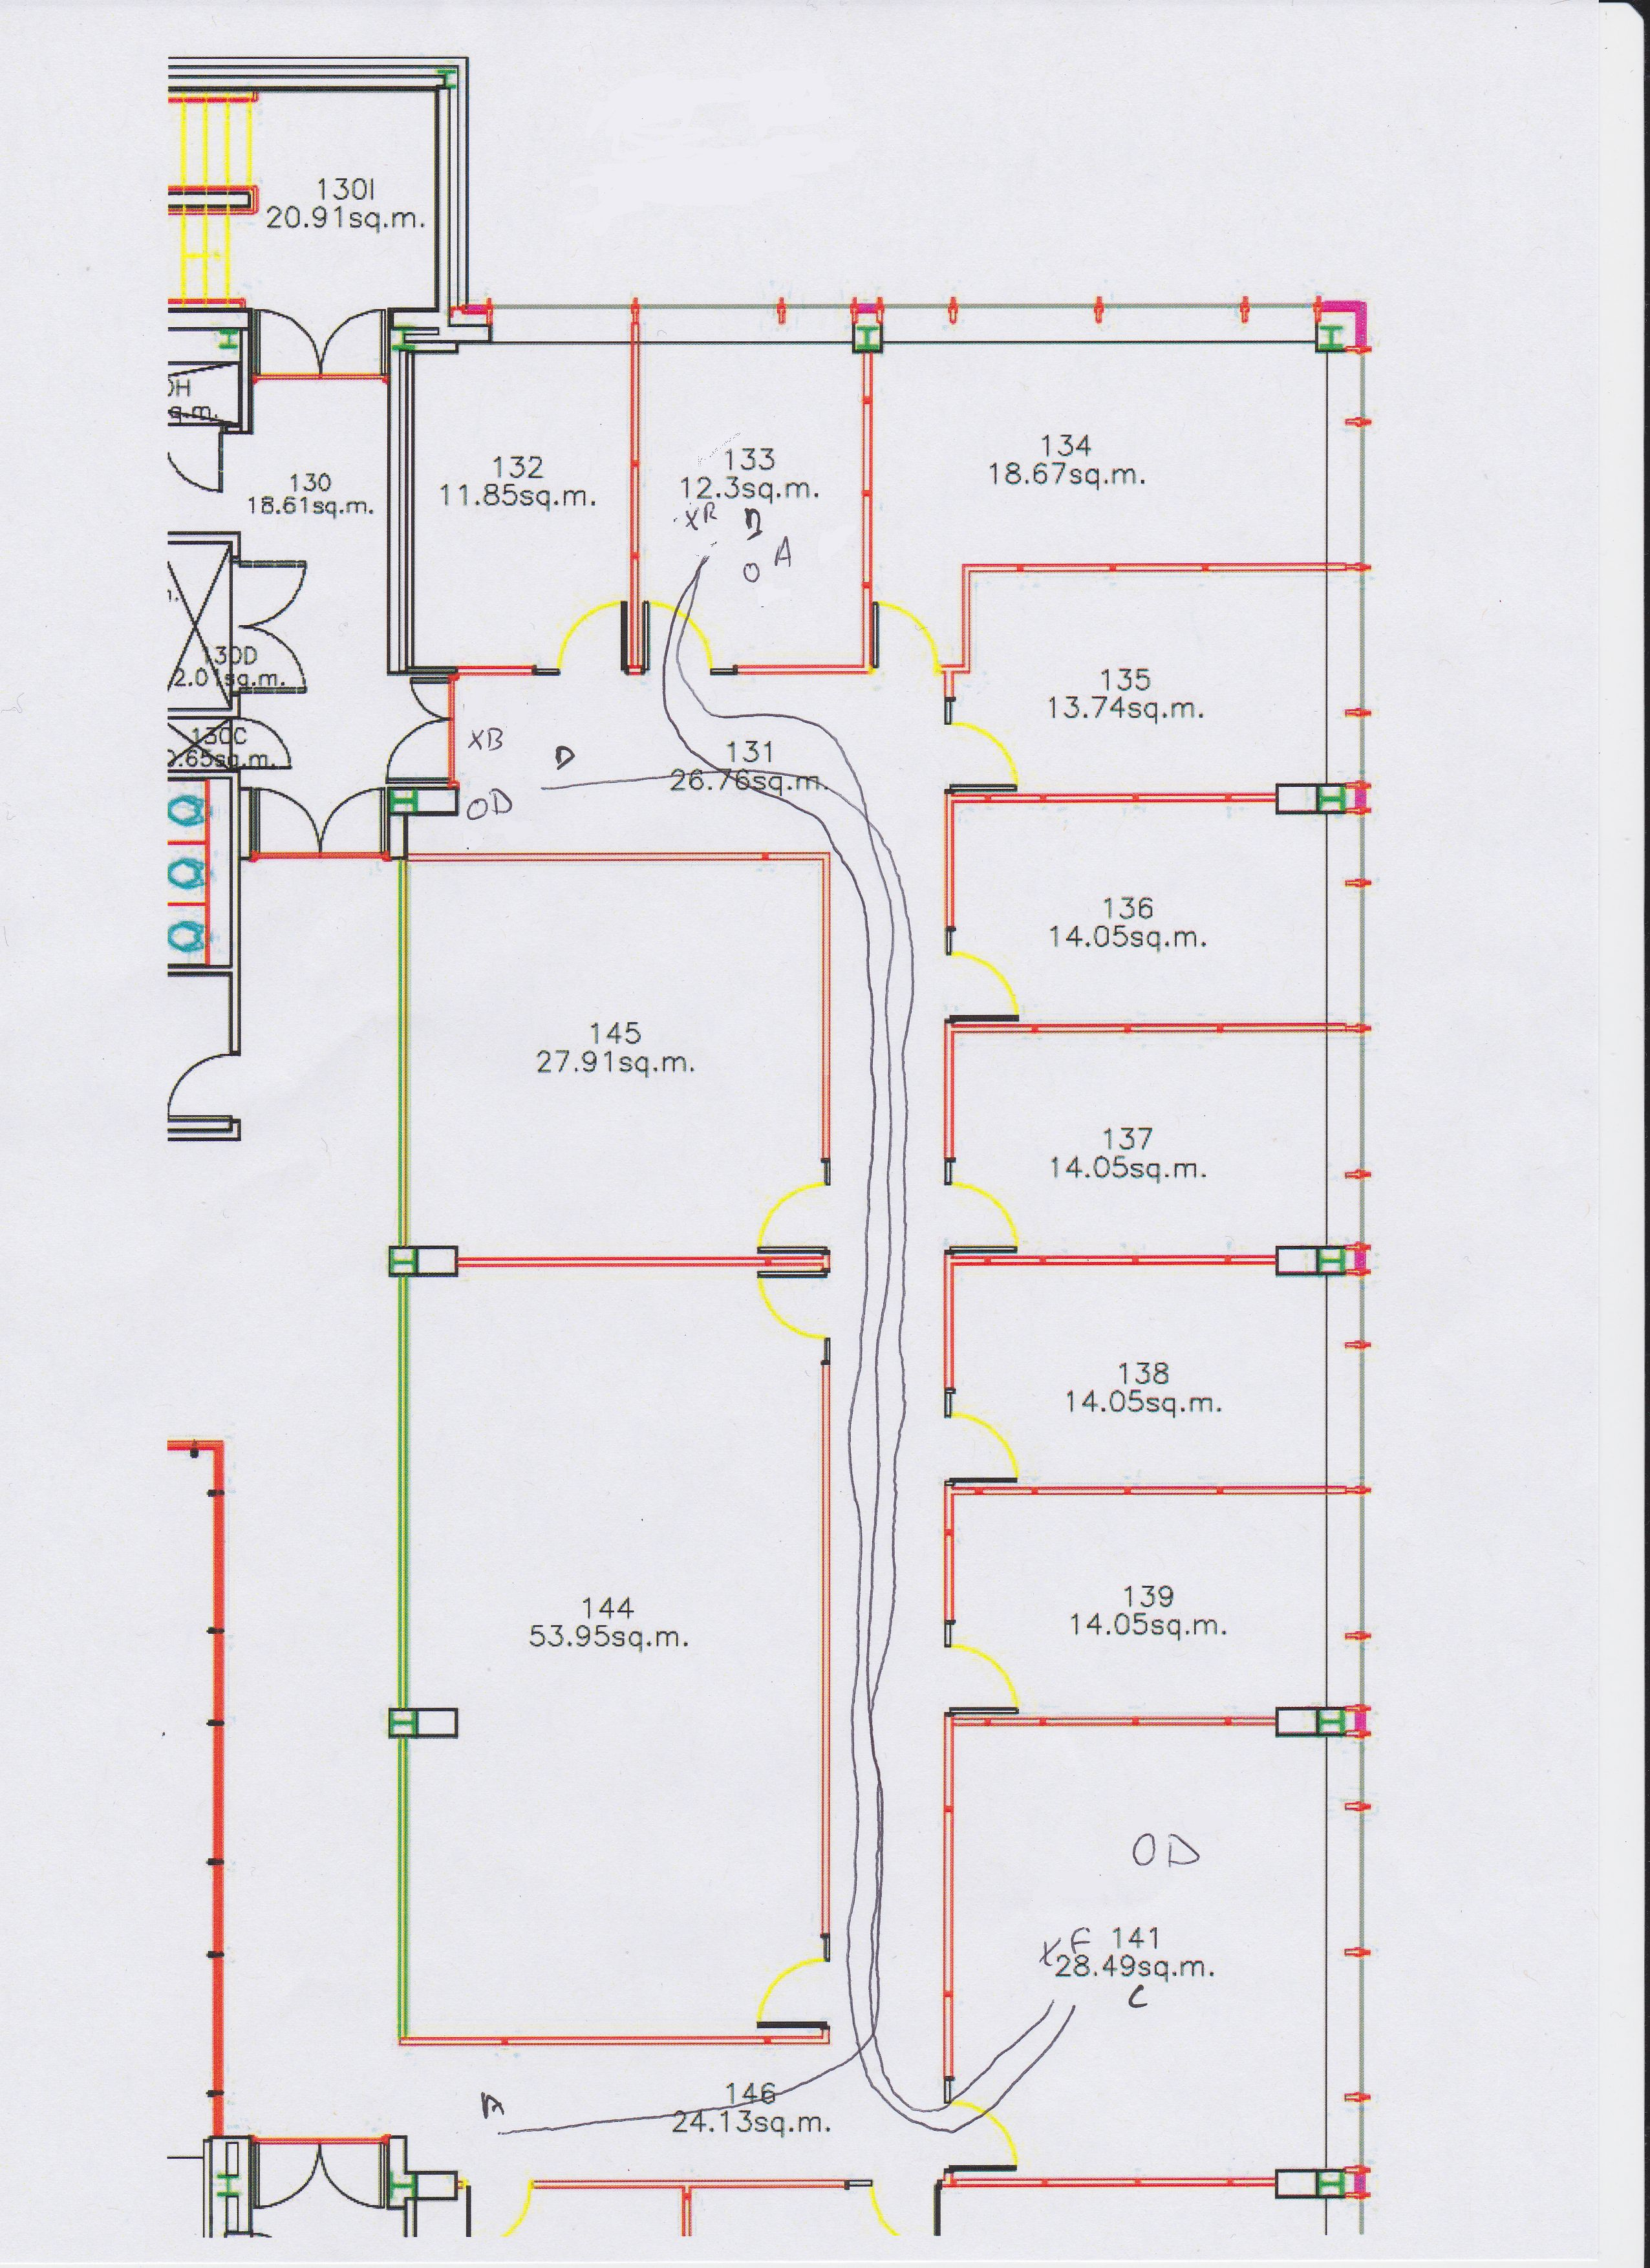
\includegraphics[width=\textwidth]{chapter5_fig/floorplan_annotated.jpeg}
			\caption{}
			\label{subfig:floorplan_annotated}
		\end{subfigure}
		\hfill
		\caption{ \textbf{\ref{subfig:floorplan}:} the floor plan, as kept in the university records, of the area that the experiment took place. This floor plan was printed and given to participants for the secondary task. \textbf{\ref{subfig:floorplan_annotated}:} the floor plan of the experiment area annotated by an operator during the secondary task.}
		\label{fig:floorplan_exp3}
	\end{figure}
    

\begin{figure}
		\centering
		\begin{subfigure}[b]{0.59\textwidth}
			\centering
			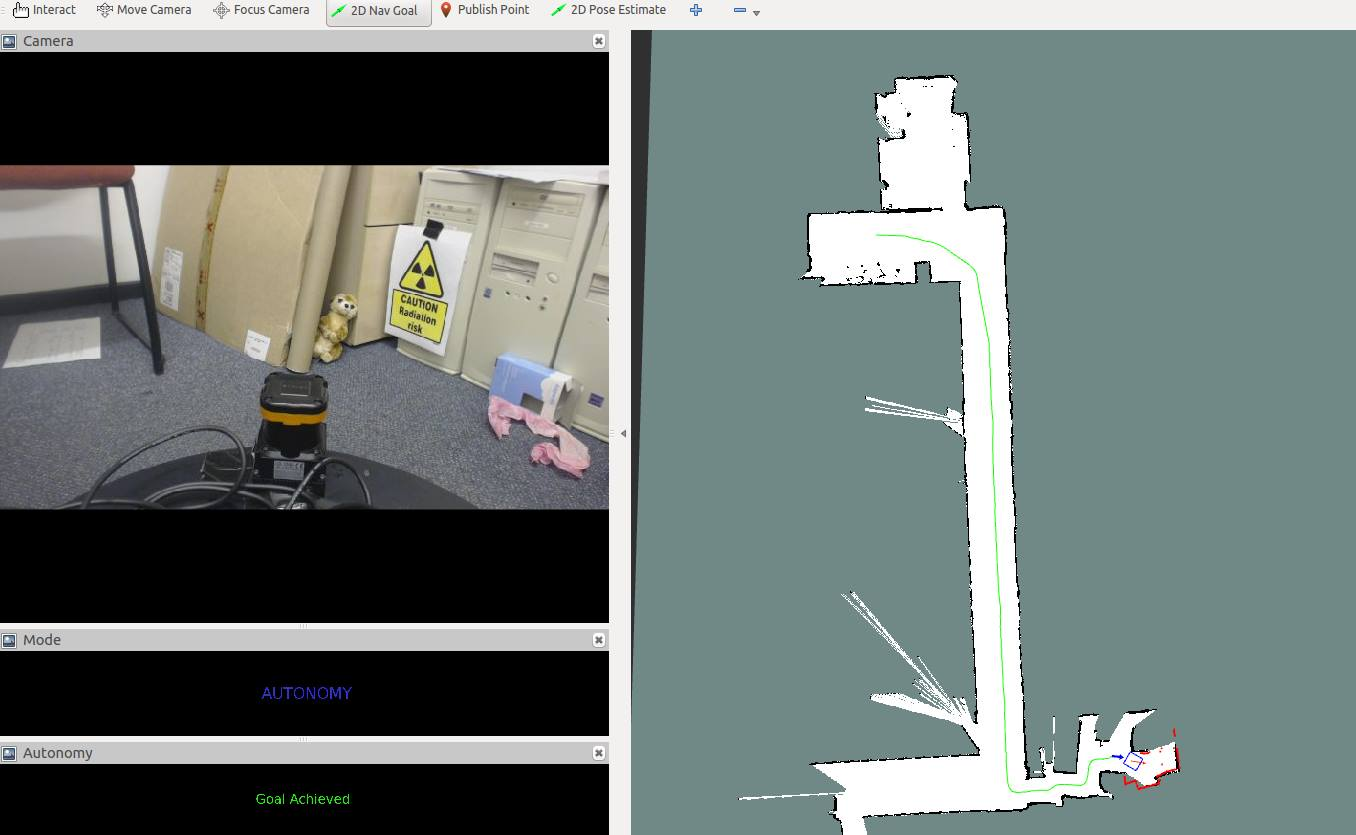
\includegraphics[width=\textwidth]{chapter5_fig/exp3_interface.jpg}
			\caption{}
			\label{subfig:interface_exp3}
		\end{subfigure}
		\hfill
		\begin{subfigure}[b]{0.3\textwidth}
			\centering
			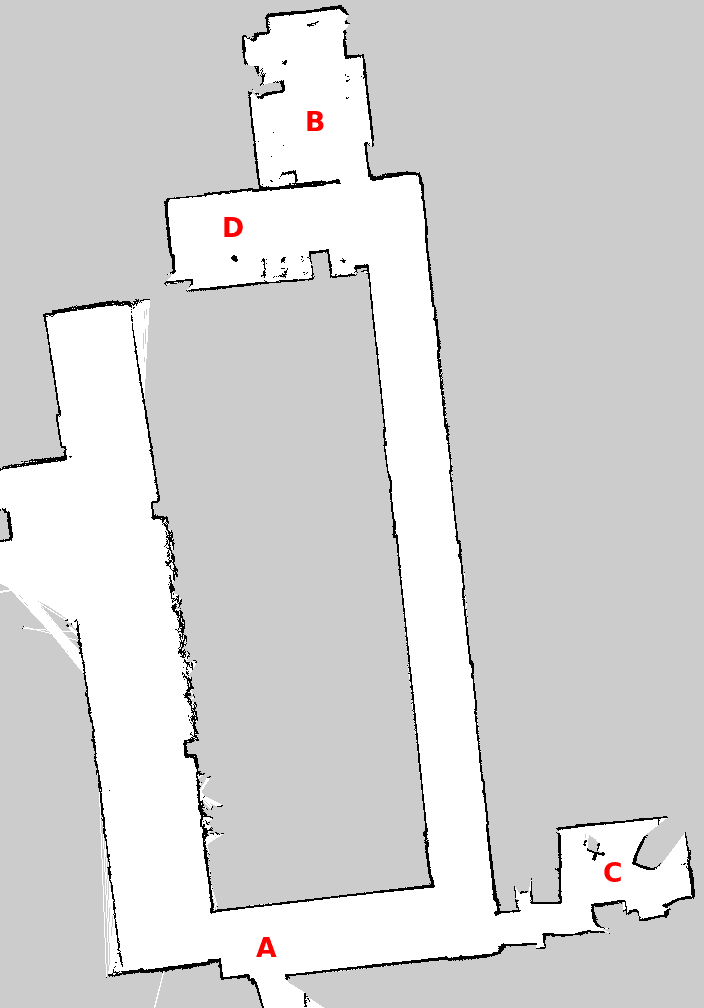
\includegraphics[width=\textwidth]{chapter5_fig/map_exp3.png}
			\caption{}
			\label{subfig:map_exp3}
		\end{subfigure}
		\hfill
		\caption{ \textbf{\ref{subfig:interface_exp3}:} The control interface as presented to the operator. \textbf{Left}: video feed from the camera, the control mode in use and the status of the navigation goal. \textbf{Right}: The map showing the position of the robot (blue footprint and red arrow), the current goal (blue arrow), the AI planned path (green line), the obstacles' laser reflections (red) and the walls (black). \textbf{\ref{subfig:map_exp3}:} The SLAM map of the arena as displayed to the human operator on the interface. Operators had to navigate in turn from point A; to B; to C; to D; and then back again to point A.}
		\label{fig:map_floor_exp3}
	\end{figure}

\subsection{Tasks and performance degradation factors}
The overall theme of the experiment was an Urban Search and Rescue (USAR) scenario. In this scenario the robot operator had to remotely control the robot in the search zone (i.e. the building) and identify the positions and the statuses of victims and potential hazards. As often is the case in real operations, we assume that some prior knowledge of the building is given to the robot operator from the authorities or any relevant organization. This is represented in the experiment by the SLAM map that appears on the interface (see Fig. \ref{subfig:map_exp3}) and by the floor plan used in the secondary task, as kept in the university's records (see Fig. \ref{subfig:floorplan}). 

The primary task was to navigate the robot between the different areas in the map in a predefined order. From point A to point B, C, D and then back to point A (see Fig. \ref{subfig:map_exp3}). In every one of those areas/points (excluding A) one victim and one hazard sign was placed. The victims were represented by stuffed animals. A meerkat represented an alive victim and a teddy-bear a dead victim (see Fig. \ref{subfig:victims}). Hazards were represented by 3 commonly used hazard sings for flammable materials, radiation, and bio-hazard (see Fig \ref{fig:hazards_exp3} and Fig. \ref{subfig:flammable})). Inside the search areas the robot had to stop in the center of the room. Then the operator would have to identify and memorize the position and status of the victim and the sign. Both the victim and the sign were visible from the center of the area and in a radius of $360$ degrees around the robot (i.e. the victim and the sign could be anywhere around the central position, but visible); no further exploration was needed.

\begin{figure}
		\centering
		\begin{subfigure}[b]{0.38\textwidth}
			\centering
			
\includegraphics[width=\textwidth]{chapter5_fig/radiation.jpg}
		\end{subfigure}
		\hfill
		\begin{subfigure}[b]{0.41\textwidth}
			\centering
			
\includegraphics[width=\textwidth]{chapter5_fig/biohazard.png}
		\end{subfigure}
		\hfill
		\caption{Two of the hazard signs used in order to denote bio-hazard and radiation risk.}
		\label{fig:hazards_exp3}
	\end{figure}

\begin{figure}
		\centering
		\begin{subfigure}[b]{0.4\textwidth}
			\centering
			
\includegraphics[width=\textwidth]{chapter5_fig/victims.jpg}
			\caption{}
			\label{subfig:victims}
		\end{subfigure}
		\hfill
		\begin{subfigure}[b]{0.45\textwidth}
			\centering
			\includegraphics[width=\textwidth]{chapter5_fig/flammable.png}
			\caption{}
			\label{subfig:flammable}
		\end{subfigure}
		\hfill
		\caption{ \textbf{\ref{subfig:victims}:} The stuffed animals representing the victims of the USAR scenario. A meerkat was representing a victim which is alive and a teddy-bear a victim which is dead. \textbf{\ref{subfig:flammable}:} The hazard sign used to denote flammable materials risk.}
		\label{fig:flammable_victims}
	\end{figure}
    
In addition to the primary task, the operator had to perform a secondary task every time the robot exited one of the search areas. This secondary task was designed to induce additional workload to the operator and degrade performance on the primary task. A pen and a paper portraying the floor's plan was placed in-front of the operator (see Fig. \ref{subfig:OCU_exp3}). When the operator was asked to perform the secondary task by the experimenter, he had to sketch on the floor plan paper (see Fig. \ref{subfig:floorplan_annotated}): a) the position of the victim denoted by a small x; b) the status of the victim denoted by a letter (A for alive, D for dead); c) the position of the hazard denoted by a small o; d) the status of the hazard denoted by a letter (R - radiation, F - flammable, and B - bio-hazard); e) the path that the robot followed from the previous visited point/area. The pen and the floor plan were placed in front of the operator and in a central position (see Fig. \ref{subfig:OCU_exp3}). This way individual differences regarding handedness (i.e. left vs right handed participants) did not biased the results. Similar tasks to the one described here, are typically required from robot operators in real world disaster response \citep{Murphy2004} as they are asked to sketch similar information for the SAR team. The speed and ability of the operators to annotate hazards, victims and paths, along with their correct status and respective positions, were the measures of secondary task performance.

The robot performance was degraded by two different degradation factors. The first factor was a box placed in one of the offices. This box was not part of the prior knowledge (i.e. the box was not in the SLAM map). The box would also narrow down the entrance to the office. For these two reasons navigation performance would degrade (i.e. the robot is either moving very slowly or is stuck), as the robot would try to plan a new path through this very tight passage and not through the obstacle. The second performance degradation factor was naturally occurring noise in the laser sensor in certain parts of the arena. This noise was due to shiny surfaces deflecting the laser's beams and it was not controlled by the experimenter. However, due to the high and semi-systematic frequency of its appearance in the specific area of the map, it was adopted as part of the experimental design. Both of these factors, naturally occurring laser noise and unknown obstacles, often occur in real scenarios as the environments are dynamic. This adds to the realism of the experiment.  

Lastly, in one of the offices the WiFi signal was weak. As a result, delays in the control commands and in SA updates in the interface (e.g. location in map, video feedback etc) occurred. This was systematic throughout all of the participants and trials. Hence, it did not constitute a confounding factor, while contributing further to the realism of the experiment.


\subsection{Participants and experimental design}
A total of 12 volunteers participated in a within-groups experimental design, as every participant performed one trial for each of the 3 control modes (i.e. teleoperation, MI, and HI). The order of the three trials was rotated between all the different permutations for different participants. This counterbalancing technique was used in order to prevent learning and fatigue effects from introducing confounding factors to the results, since every participant performed all three trials. Additionally, for the secondary task, the signs, the victims, and their positions were randomized in every trial. Again, this was in order to eliminate any learning effects. A prior experience questionnaire showed, as in our previous experiments, that the majority of the participants were experienced in playing video games. Moreover, 8 out of the 12 participants have participated in our previous experiment. 

Participants underwent extensive standardized training, similar to our previous experiment. Due to space constrains a sub-region of the experiment's area was used for the training. In order for the participants to proceed with the experiment they had first to demonstrate their abilities by completing three standardized test trials, one for every control mode. These trials mimicked the actual experimental trials (i.e. same primary and secondary tasks). The training and the test trials ensured that all participants had attained a common minimum skill level in operating the robot. 

Participants were instructed to perform the primary task (controlling the robot to search the areas) as quickly and safely (i.e. avoiding collisions) as possible. Additionally they were told that when instructed to perform the secondary task (i.e. annotating information regarding victims, hazards, and paths), they should do it as quickly and as accurately as possible. They were explicitly told that they should give priority to the secondary task over the primary task and should only perform the primary task if the workload allowed. Lastly, participants were told that the best performing individuals in each trial would be rewarded with an extra gift voucher. However, they were not informed about how the best performing participants would be decided, as it would have had them biased towards specific factors. The purpose of this extra gift voucher was to provide an incentive for participants to achieve the best performance possible on both primary and secondary task.

At the end of each trial, participants had to complete an online NASA Task Load Index (NASA-TLX) questionnaire. As in our previous experiments, NASA-TLX was used to rate the level of difficulty and workload participants experienced during each trial.


\subsubsection{Results}
A repeated measures one-way ANOVA was used. The independent variable was the control mode with three levels: teleoperation; HI; and MI. In the cases that sphericity assumption was violated a Greenhouse-Geisser correction was used with the ANOVA. For pairwise comparisons after a significant ANOVA result, Fisher's least significant difference (LSD) test was used do determine the conditions that differed. Similar to the rest of the thesis, we consider a result to be significant when it yields a $p$ value less than $0.05$. We also report on the statistical power of the results and on the effect size using $\eta^2$. 

% PRIMARY TIME
ANOVA for \textit{primary task completion time} (see Fig. \ref{subfig:primary_metrics_exp3}) showed overall significantly different means with \textit{$F(2, 22) = 7.382$,  $p < .01$, $power > .9$, $\eta^2 = .402$} between HI variable-autonomy (\textit{$M = 327.9$ $sec$, $SD = 23.38$}), MI (\textit{$M = 349.5$ $sec$, $SD = 35.95$}) and teleoperation (\textit{$M = 366.3$ $sec$, $SD = 36.26$}). Pairwise comparison reveals that HI performed significantly better (i.e. lower mean completion time) than teleoperation (\textit{$p < .01$}). MI primary task completion time was statistically in the same level as teleoperation and HI (\textit{$p > .05$}).
 
% COLLISIONS
The effect of control mode on the number of \textit{collisions} was not significant (\textit{$F(2, 22) = .786$, $p > .05$, $\eta^2 = .067$, $power < .8$}). Teleoperation had on average \textit{$M = 0.25$ ($SD = 4.52$)} collisions, MI had \textit{$M = 0.08$ ($SD = .289$)} collisions, and HI had \textit{$M = 0.08$ ($SD = .289$)} collisions.

	\begin{figure}
		\centering
		\begin{subfigure}[b]{0.46\textwidth}
			\centering
			\includegraphics[width=\textwidth]{chapter5_fig/exp3_primary_metrics.png}
			\caption{}
			\label{subfig:primary_metrics_exp3}
		\end{subfigure}
		\hfill
		\begin{subfigure}[b]{0.48\textwidth}
			\centering
			\includegraphics[width=\textwidth]{chapter5_fig/exp3_secondary_time.png}
			\caption{}
			\label{subfig:secondary_time_exp3}
		\end{subfigure}
		\hfill
		\caption{\textbf{\ref{subfig:primary_metrics_exp3}:} primary task mean time-to-completion (green) and score combining time and collisions penalty (blue). \textbf{\ref{subfig:secondary_time_exp3}:} mean secondary task completion time. In all graphs the error bars indicate the standard error.}
		\label{fig:exp3_primary_secondary}
	\end{figure}
	
% PRIMARY SCORE
Similar to our previous experiments the \textit{primary task score} (see Fig. \ref{subfig:primary_metrics_exp3}) was calculated in order to capture any speed-accuracy trade-offs in the primary task. The primary task score was calculated by adding a time penalty of \textit{$10$ $sec$} for every collision onto the primary task completion time for each participant. ANOVA analysis showed that control mode had a significant effect on the primary task score (\textit{$F(2, 22) = 8.724$, $p < .01$, $power > .9$, $\eta^2 = .442$}). As expected due to the small number of collisions, LSD pairwise tests showed very similar results with the primary task completion time. The HI controller (\textit{$M = 328.8$, $SD = 22.42$}) significantly (\textit{$p < .01$}) outperformed pure teleoperation (\textit{$M = 368.8$, $SD = 35.57$}). The primary task score for MI controller (\textit{$M = 350.3$, $SD = 34.9$}) was in the same level (i.e. no statistical difference found) as pure teleoperation and HI (\textit{$p > .05$}). 

% SECONDARY TIME
\textit{Secondary task completion time} (see Fig. \ref{subfig:secondary_time_exp3}) refers to the total time per trial that the participants took to complete the full annotation in the floor footprint. As a full annotation is defined a sketch that has annotated positions, statuses and paths for all the three search areas. ANOVA with \textit{$F(2, 22) = 0.68, p > .05 , power > .85$, $\eta^2 = .058$}, did not suggested a significant difference between the mean secondary task completion times for the different controller. MI (\textit{$M = 54.8$ $sec$, $SD = 20.16$}) , HI (\textit{$M = 54$ $sec$, $SD = 12.86$}), and teleoperation (\textit{$M = 60.3$ $sec$, $SD = 16.37$}) did not show statistical differences.

	\begin{figure}
		\centering
		\begin{subfigure}[b]{0.49\textwidth}
			\centering
			\includegraphics[width=\textwidth]{chapter5_fig/exp3_NASA-TLX.png}
			\caption{}
			\label{subfig:nasa-tlx_exp3}
		\end{subfigure}
		\hfill
		\begin{subfigure}[b]{0.49\textwidth}
			\centering
			\includegraphics[width=\textwidth]{chapter5_fig/exp3_secondary_mistakes.png}
			\caption{}
			\label{subfig:secondary_mistakes_exp3}
		\end{subfigure}
		\hfill
		\caption{\textbf{\ref{subfig:nasa-tlx_exp3}:} NASA-TLX score showing the overall trial difficulty-workload as perceived by the operators. \textbf{\ref{subfig:secondary_mistakes_exp3}:} Secondary task total number of errors for each trial.}
		\label{fig:nasa_secondary_mistakes_exp3}
	\end{figure}

% SECONDARY MISTAKES
The \textit{secondary task number of errors} was measured. As a position error was defined an annotation not representing the true position of a victim or hazard with relative accuracy. As a status error was defined an annotation not representing the correct status, e.g. victim annotated alive (i.e. meerkat) when is it in-fact dead (i.e. teddy-bear). As a path error was defined: a) a path that was not annotated; b) a path that was heavily colliding with the walls in the floor plan; c) a not accurately depicted path. In a real situation the rescue team should be able to find the victims which are alive, be aware of any hazards and their nature. This should happen by following the path and the position annotations provided and by using common sense regarding space orientation. This is represented in our experiment by the secondary task errors. No significant differences were observed between the different control modes with respect to the number of secondary task errors (see Fig. \ref{subfig:secondary_mistakes_exp3}) according to ANOVA (\textit{$F(2,22) = .789, p > .05 , power < .8$, $\eta^2 = .067$}). Participants had \textit{$M = 1.42$ ($SD = 1.62$)} errors in teleoperation, \textit{$M = .83$ ($SD = 1.03$)} in HI trial, and \textit{$M = 1.5$ ($SD = 1.314$)} in MI.

% NASA-TLX
Control mode had a significant effect on \textit{NASA-TLX scores} (see Fig. \ref{subfig:nasa-tlx_exp3}) as suggested by ANOVA (\textit{$F(1.263,13.896) = 5.001, p < .05 , power = .603$, $\eta^2 = .313$}). Pairwise comparisons showed that teleoperation (\textit{$M = 38.9$, $SD = 17.4$}) was perceived as harder (i.e. more workload) compared to HI (\textit{$M = 25.9$, $SD = 12.39$}) with $p < 0.05$ and marginally harder than MI (\textit{$M = 29.9$, $SD = 14.94$}) with $p = 0.05$. HI variable autonomy is perceived as having the same difficulty as MI ($p > 0.05$). 


% Number of LOA switches
The mean \textit{number of LOA switches} in HI and in MI were compared using a paired samples t-test. The reason for using a paired samples t-test is that the experiment had a within-groups design, i.e. we expect some correlation on the results given that the same participants performed both conditions. The mean number of LOA switches in MI (\textit{$M = 15.08$, $SD = 5.73$}) was significantly higher than the number of LOA switches in HI (\textit{$M = 9.08$, $SD = 3.42$}), as shown by the t-test $t(11) = -4.076 , p < 0.01$. Using Pearson's correlation, no correlation was found in mean LOA switches between HI and MI ($r(10) = .472, p >. 05$). Given that the correlation assumption of paired samples t-test does not hold true, we used a independent samples t-test to validate the result further. Again, the means of HI and MI are significantly different, $t(22) = -3.115 , p < 0.01$. The mean number of LOA switches in MI due to robot's initiative is \textit{$M = 3.42$, ($SD = 1.83$)}. The histograms illustrating the number of LOA switches in MI and HI can be seen in Fig. \ref{fig:histogram_hi_exp3} and Fig. \ref{fig:histograms_mi_exp3}.

\begin{figure}
	\centering
	\includegraphics[width=0.49\columnwidth]{chapter5_fig/histogram_loa_hi_exp3.png}
	\caption{Histogram showing the number of human operators who chose to make various different numbers of LOA switches during HI.} 
	\label{fig:histogram_hi_exp3}
\end{figure}


	\begin{figure}
		\centering
		\begin{subfigure}[b]{0.45\textwidth}
			\centering
			\includegraphics[width=\textwidth]{chapter5_fig/histogram_loa_mi_exp3.png}
			\caption{}
			\label{subfig:histogram_lao_mi_exp3}
		\end{subfigure}
		\hfill
		\begin{subfigure}[b]{0.45\textwidth}
			\centering
			\includegraphics[width=\textwidth]{chapter5_fig/histogram_loa_mi_ai_exp3.png}
			\caption{}
			\label{subfig:histogram_lao_mi_ai_exp3}
		\end{subfigure}
		\hfill
		\caption{\textbf{\ref{subfig:histogram_lao_mi_exp3}:} Histogram showing the number of human operators who chose to make various different numbers of LOA switches during MI. \textbf{\ref{subfig:histogram_lao_mi_ai_exp3}:} Histogram showing the number of human operators and the number of LOA switches initiated by the fuzzy MI controller.}
		\label{fig:histograms_mi_exp3}
	\end{figure}


\subsubsection{Discussion}
Regarding performance in the primary task, HI controller outperformed teleoperation both in terms of score and time-to-completion. This is important evidence further reinforcing our findings in \citep{Chiou2016} (see also Chapter \ref{chapter4:HI}) that HI variable autonomy outperforms individual LOA such as teleoperation and autonomy. Of particular importance is that this evidence came from conducting a real world scenario in which we aimed for realism; not restricting potential degradation factors (e.g. naturally occurring noise or communication issues), while at the same time having a controlled experiment. 

In contrast to our previous experiment (see Section \ref{chapter5:experiment2_2}), results from the use of MI controller are difficult to interpret. A trend can be seen as MI performed better than teleoperation in primary task, however the result was not statistically significant. Comparison between HI and MI does not lead to safe conclusions, as no statistical difference was found. We believe this is due to authority conflict between the operator's and the robot's initiative regarding LOA switching. This conflict arose from a restriction that the MI controller has. It is designed on the assumption that the agent who is in control (e.g. the robot or the operator) follows relatively close the path yielded from the expert planner. Our experiment was designed to control for exploration strategies by restricting operators in only visiting the center point of the offices/areas, as victims and hazards were visible from that point. However, there were occasions that operators decided to engage in some exploration or follow a less restricted path (i.e. compared to the one the expert planner yielded). For example operators that decided to move closer to a hazard sign in order to see the letters more clear or in order to improve lighting conditions on the sign. Another example is operators that struggled to pass through the narrow passage created by the unseen object. In such cases the MI controller inferred a performance drop or a deviation from the navigation goal; as a result robot's initiative switched to autonomy. At the same time, if operators have not yet finished their action, they would switch back to having control (i.e. teleoperation). This is further reinforced by participants' feedback. Many of them noted that they would trust the MI controller as there were cases in which the controller switched LOA in a meaningful way. However, they felt restricted from driving freely and they also felt the controller was intrusive at times. Others noted that they felt the MI capabilities were redundant, given that HI controller was easy enough to use.

Every time a LOA switch takes place, the fuzzy MI controller re-initializes the error exponential moving average for a time period of $3.2$ $sec$. During this period the controller cannot initiate a LOA switch. In essence, this period of time acts as a minimum time between robot controller initiated switches. Despite this period, the conflict for control have not been avoided, suggesting that it is happening on a bigger time scale (e.g. several seconds). Instead, this conflict for control between the robot and the operator can be avoided to a large extent by MI controllers that are context aware. Imagine the following two situations and a MI controller that is not context aware. In the first situation the robot is idle (i.e. no progress towards the goal) because the operator is neglecting it in order to perform a secondary task. The performance error measured by the controller is the maximum. In the second case the robot is stuck in a corner and the operator is reversing in order to escape the enclosure. Similar to the previous situation the performance error is the maximum. A MI controller that does not take context into account, would initiate a LOA switch in both cases. In the first case the switch into autonomy would be beneficial as the robot was idle. In the second case it can potentially lead to a collision as the operator is in the middle of a maneuver. It can also lead to a control conflict as the operator can try to take control back in order to complete the maneuver. A context aware controller would have been able to distinguish that although in both cases the performance error was large, the situation was different. Hence, in the second case a LOA switch wouldn't have happened. Our MI controller in this specific example, is aware that the large error while the robot is reversing, potentially means maneuvering to escape an entrapment (see fuzzy rule base in Section \ref{chapter5:fuzzy_controller}). However, with cases such the ones discussed in the previous paragraph (e.g. operator performing exploration), our controller is not able to cope. We identify context awareness as a major challenge for robotics MI systems. We believe that fuzzy controllers can help towards this direction as they can be expanded with expert knowledge regarding context. Lastly, system transparency is another factor that might positively contribute towards tackling LOA switching conflicts. 

The above evidence suggesting a control conflict, is in accordance with the fact that MI had significantly more LOA switches compared to HI. In contrast to the results of Section \ref{chapter5:experiment2_2} in which LOA switches of MI and HI were highly correlated, in the experiment reported here no correlation was found. This further reinforces the notion that possibly these extra LOA switches steam from the robot-operator conflict for control as they would switch LOA back and forth. Similarly, a number of LOA switches initiated from the robot they might be due to this control conflict. Further HRI specialized studies are required in order to investigate the phenomenon better as this conflict is a major challenge to overcome for MI systems. Lastly, the fact that the number of LOA switches is relatively high for both HI and MI, is in accordance with the findings of our previous two experiments (see Chapter \ref{chapter4:HI} and Section \ref{chapter5:experiment2_2}). These findings suggested that the high number of LOA switches was due to reasons beyond performance (e.g. personality traits).

The secondary task performance (i.e. time-to-completion and number of errors) were on the same level for all three control modes. This evidence suggests that LOA switching capabilities did not have any effect on the secondary task performance. This is similar to the evidence of the experiment on Chapter \ref{chapter4:HI}, in which teleoperation and HI performed equally on the secondary task. It also reinforces the possibility that the improved secondary task performance on our initial MI controller evaluation (compared to HI - see Section \ref{chapter5:experiment2_2}), was due to learning effects. However because: a) the secondary task on Chapter \ref{chapter4:HI} and on Section \ref{chapter5:experiment2_2} is different from our current task; and b) the statistical power (i.e. the probability that a significant difference will be found if it exists) on our number of errors calculations is low; a safe conclusion cannot be reached.

Regarding the difficulty/workload of the trials, NASA-TLX showed that teleoperation was perceived as the most difficult control mode compared to HI and MI. This suggests, similar to the findings of Chapter \ref{chapter4:HI} (see also \citep{Chiou2016}), that the use of variable autonomy can alleviate operators from the burden of control. Perceived difficulty for MI and HI was on the same level according to the pairwise comparisons. This is in contrast to the findings of Section \ref{chapter5:experiment2_2} in which MI found to be easier than HI. However, due to the low statistical power, the possibility of MI and HI differing is not excluded.


 
\section{Conclusion and impact}
This chapter presented the expert-guided approach to designing MI controllers and conducting evaluation experiments. It also presented a novel MI controller and its experimental evaluation by both using a high fidelity simulator and in a realistic real world scenario.

The proposed controller used expert knowledge taken from data on how human operators switch LOA during HI trials. Using this knowledge and an online performance metric that represents the effectiveness of goal directed motion, the controller was able to measure performance; infer if a LOA switch was needed; and switch LOA. 

Evidence from our initial evaluation, showed the potential advantages of MI control. The MI controller was found to outperform HI control in terms both of primary and secondary task performance (see Fig. \ref{fig:primary_secondary_exp2_2} and Section \ref{chapter5:sim_results_system}). This in turn means that MI outperforms control modes that lack any LOA switching capabilities such as teleoperation and autonomy.

The second evaluation extended our experimental framework towards a less controlled and more realistic setting. The MI controller was used in a real robot performing in a USAR scenario. Results regarding performance advantages of MI over HI were less conclusive compared to the initial evaluation. However, the experiment yielded significant new insight into challenges and problems which need to be overcome in the design of MI systems. The difficulty to interpret the results was partially due to variance and poor statistical power in some of the statistical calculations. This can be tackled in future experiments by: a) using a higher number of participants; b) using a bigger robot arena; c) adjusting the difficulty of the primary and secondary tasks towards making them more difficult. However, the major confounding factor in the results, was the conflict for control that arose between the operator and the AI. This led operators and the AI to confusion on what they should do as the LOA was switching back and forth between autonomy (i.e robot in control) and teleoperation (i.e. human in control). We believe this control conflict is one of the major challenges for future MI control research. Furthermore, context aware MI controllers as a way to overcome this conflict, is another major challenge to be tackled. However in the general case, MI control has its merits as the operators might not always been able to switch LOA if needed e.g. loss of communication with the robot or a sudden event impairing the operator temporary. 

Lastly, the USAR experiment provided important real world evidence that variable autonomy control in the form of HI significantly outperforms teleoperation in a navigation task. This is in accordance to our previous findings (see Chapter \ref{chapter4:HI}) and denotes that human operators successfully use HI capabilities to overcome various performance degrading factors and situations. Lastly, some further evidence are provided to further support the hypothesis that operators switch LOA for reasons other than performance. 

Overall, we believe that this chapter has made a number of significant contributions to the MI research on mobile robots: a) proposed a framework for designing MI controllers; b) proposed a novel MI system; c) provided evidence on the benefits of MI control while identifying the shortcomings that constitute open challenges for the research field.


\chapter{CONCLUSIONS AND FUTURE WORK}
\label{chapter6:conlcusion}
This thesis addressed the problem of improving teleoperated mobile robots by the use of variable autonomy. Variable autonomy allows for human and robot capabilities to be used on demand, e.g. in order to improve task performance. More specifically this thesis aimed to tackle the problem of dynamically switching LOA using either HI or MI control. Surprisingly, previous research on variable autonomy has not fully explored fundamental questions such as which is the optimum choice of LOA at a given moment; which factors affect this choice; and most importantly how this will be used to address the transition between LOAs? This thesis investigated these problems by using a rigorous multidisciplinary experimental framework based on methodologies from psychology, human factors, engineering and computer science.

In our initial investigation a real world experiment was conducted in which a remotely controlled robot performed a navigation task. This experiment illustrated the intrinsic difficulty in conducting variable autonomy experiments with human participants. Difficult confounding factors such as individual differences in personality traits; experience on operating robots or playing video games; and map exploration strategies; yielded difficult to interpret results due to the big variance between different human operators. However, lessons learned from this experiment allowed us to construct a systematic experimental framework using meaningful secondary tasks and other performance degrading factors. 

In our second investigation we designed a HI system which allowed operators to switch LOA dynamically. An experiment to evaluate the HI control was conducted using a high fidelity simulator. The HI control proved advantageous in various circumstances compared to teleoperation and autonomy, resulting in better performance on the navigation task. Moreover, HRI evidence suggested that operators switched LOA for reasons beyond task performance, e.g. personal preferences and trust in the system.  

Next, using the insights from our previous experiments we proposed an expert-guided approach for the design of MI controllers. Two MI controllers based on this approach were designed, a threshold controller and a fuzzy controller. The fuzzy controller was evaluated in two different experimental settings: a) using an identical experimental protocol with our previous HI experiment; and c) in a real world USAR scenario. In the former, MI control outperformed HI both in primary and in secondary tasks, providing evidence that a robot controller capable of taking initiative can be advantageous. The latter experiment allowed us to identify two major challenges for MI control: a) the conflict for control between the operator and the robot; and b) context awareness. Lastly, evidence from these experiments further reinforced the findings that HI outperforms teleoperation and that operators switch LOA based on a variety of factors (i.e. not just based on performance). 

\section{Contributions}
The research conducted for this thesis has provided the following contributions to the fields of variable autonomy and HRI:

\begin{itemize}

	\item \textbf{A systematic experimental framework for validation of variable autonomy robotic systems:} Previous research on variable autonomy robotic systems was lacking a rigorous and systematic experimental framework. More specifically, much of the research was not carefully controlling for potential confounding factors. Those factors included the absence of standardized training; uncontrolled environments or experimental conditions; and experimental designs that did not controlled for human factors variability. Additionally, previous research was lacking formalized and detailed experimental paradigms. In contrast, we investigated variable autonomy by using a systematic experimental framework that exploited methodologies from psychology; human factors; engineering; and computer science. Of particular importance to the contributed experimental framework is the use of quantifiable and repeatable degradation factors both for the operator and the robot. Overall, our proposed paradigm allows for meaningful and repeatable scientific inference. 
    
	
	\item \textbf{A Human-Initiative (HI) variable autonomy robotic system and its evaluation:} This thesis presented a HI controller in which the human operator can dynamically switch LOA between teleoperation (i.e. direct joystick control) and autonomy (i.e. robot navigates autonomously towards waypoints selected by the human). Although some HI systems exist in literature, compared to our work they lack in one or more of these three key aspects: a) the HI controller is not able to switch LOA on-the-fly; b) the HI controller is not evaluated experimentally; c) the evaluation does not follow a systematic experimental protocol (e.g. controlled performance degradation factors) that allows for a rigorous analysis on the advantages of HI compared to control modes such as teleoperation or autonomy. In this thesis we presented for the first time to the best of our knowledge, statistically validated empirical evidence that HI outperformed teleoperated or autonomous systems in various circumstances. More specifically, HI performed consistently better in navigation tasks (i.e. faster time-to-completion and less collisions). This evidence came from using our rigorous experimental framework in two separate cases: a) in a highly controlled experiment using a simulated robot that allowed for a high degree of repeatability; b) in a real world experiment mimicking a USAR scenario. This allowed HI to be evaluated in a more realistic and less controlled setting.
    
    \item \textbf{An informed framework for designing expert-guided robotic MI control systems:} Literature is almost completely lacking truly MI robotic systems in which both the robot and the operator can initiate actions. As a result the literature lacks reporting any suggestions and insights on how to design such systems. We contributed by providing a framework for designing expert-guided MI controllers. Such controllers are based on the existence of an "expert" (e.g. by using expert knowledge or an expert planner) which is able to control the robot in a close-to-optimal manner in that task. The framework is informed by our previous experiments, using our variable autonomy experimental paradigm.
    
	\item \textbf{A novel MI robotic system and its evaluation:} We designed and tested a novel MI controller which gives the ability and authority to both the operator and the robot to switch between different LOA. To the best of our knowledge, this is the first time in literature that a MI controller able to switch LOA is designed and evaluated. To achieve this our controller uses an online performance metric, namely effectiveness of goal directed motion, and expert knowledge in the form of fuzzy logic. This knowledge was mainly extracted using machine learning techniques such as grid search on data from human operators switching LOA based on judgment (i.e. HI control data). Additional expert knowledge was used on simplified context awareness, in the form of heuristic fuzzy rules. The use of fuzzy logic gives to the controller the advantage of tackling more effectively the inherently complex problem of LOA switching. It allows for future improvements by: a) the addition of new linguistic variables; b) the extension of the fuzzy rule base; c) the addition of new output states. Also, a rigorous evaluation of the MI robotic system was performed. We reported on statistically validated empirical evidence regarding the advantages of the MI control in various circumstances, compared to HI and teleoperation. This was in regard to performance on navigation tasks, cognitively demanding secondary tasks, and perceived workload. We consider the designed MI controller and its evaluation as the primary contribution of this thesis.
    
    \item \textbf{Empirically identifying two major challenges for MI control:} The rigorous evaluation of the MI system allowed us to identify and report on empirical evidence and insights on two major challenges for MI robotic systems. The first challenge relates to the HRI domain. It is the conflict for control between the operator and the robot, arising from the fact that the robot was switching LOA against operator's will. This led to LOA switching back and forth between teleoperation and autonomy as both agents were trying to be in control. The main reason was that the robot was detecting performance degradation without taking context into account. This included cases in which the operator was performing some necessary action which the robot was ignoring, e.g. exploration. This control conflict can be tackled by MI controllers that are context aware, e.g. by detecting the reason behind degraded performance. We identified the design of context aware controllers as the second major challenge for robotics MI research.
	
    \item \textbf{An analysis on the HRI of the HI and MI systems:} Interactions between human operators and variable autonomy robotic systems remained predominantly unexplored in the literature. This is especially true for systems that allow dynamic LOA switching. In contrast, this work provided systematic analyses on how human operators interacted and used the variable autonomy controllers (i.e. HI and MI). We reported on metrics such as time spent in each LOA; frequency of LOA switches; perceived workload; and their correlation with system performance and between each other. Our findings provide evidence on two directions: a) when operators are trained accordingly, they are able to take advantage of the variable autonomy capabilities and improve system's performance; b) most of the HRI boils down to the understanding of the system, the personality traits; and preferences of the individuals. For example participants may switch LOA more often that it is necessary for performance, when they anticipate a performance drop. Also participants may use more autonomy or teleoperation depending on the perceived difficulty and on their preference to a more direct or a more laid back operation style. 
     
\end{itemize}


\section{Future work}
Here we present several directions for future research. Most of the future research should aim primarily in tackling the control conflict between the human operator and the robot controller. The suggested future research follows:

\begin{itemize}
   
\item \textbf{Expand/modify the fuzzy MI controller to include more context awareness:} We identified context awareness as one of the major challenges and shortcomings of MI control. A more context aware controller will contribute towards tackling control conflicts between the operator and the MI controller. Furthermore, context awareness will allow the MI controller to cope with more complex tasks that require the robot to move in a less restricted way, e.g. exploration tasks or tasks beyond navigation. A good starting point would be to expand the fuzzy controller in two directions: a) adding more input variables in order to add more information to the fuzzy controller; and b) adding more rules to the fuzzy rule base. Potential input variables may include joystick activity or an online workload metric which will allow the controller to have information on the status of the operator. Information on the status of the operator is of great importance as would enable the robot to infer what the operator is performing, e.g. the operator is under heavy workload or the operator is controlling the robot despite a measured performance drop. By using such metrics the fuzzy rule base can play the role of a model that the robot has about operator's behavior. Additionally, the fuzzy rule base should be expanded with heuristic rules based on the expert knowledge of the experimenters and the operators. Careful analysis and playback of all the data gathered during this thesis could inform these heuristic rules.
    
 \item \textbf{Conduct further human factors and HRI studies of HI and MI systems:} In this thesis we provided analyses on the interactions between the operators and the variable autonomy control systems (i.e. HI and MI). Our findings should act as a starting point for further HRI and human factors analyses. Future research should aim to investigate the factors that govern operators' LOA switching patterns. Firstly, the experimental framework must be shifted to facilitate more in-depth HRI studies. This can be achieved by designing the experiments specifically to address human factors issues instead of focusing on system performance. Secondly, based on the findings reported in this thesis, we propose for the future research to focus on investigating how the HRI is affected by: a) personality traits such as hands-on/hands-off operating approach and tendency to give control or to be in control; b) the trust of the human operator of the robot controller; c) operator's experience and understanding in operating the system.  
 
\item \textbf{Expand the experimental paradigm to investigate task- and context-based allocation of control:} This thesis was primarily focused on navigation. Next, research should focus on expanding the experimental paradigm to include: a) more complex navigation tasks; and b) multiple tasks that allow cooperation between the operator and the robot. Regarding the navigation tasks, a less restricted search task (e.g. free exploration) would be the next step. Tasks that require the cooperation or division of labor between the robot and the human in order to be accomplished better are particularly interesting and need to be integrated into the framework. These tasks would allow the investigation of the collaborative potential that variable autonomy offers between the operator and the robot. They should be build upon the already implemented navigation task. An example is a search task in which the human-robot team will need to explore an area and search for victims similar to the experiment described in Section \ref{chapter5:experiment3}. However, in this particular USAR scenario, one agent can be in control of navigation while the other deploys its capabilities to identify victims, hazards, and evaluate their condition. Control allocation and the LOA will not be static. Instead, variable autonomy will enable task- and context-based allocation of control for improved performance. For example a robot equipped with infrared cameras should be responsible for the identification of victims under dim lighting conditions while the operator is performing exploration. When the exploration is over, the robot can take control of navigation while the operator is conveying information to the rescue team.
 
 \item \textbf{Use of physiological measures for operator's cognitive state inference:} The use of physiological measures to infer operator's status (e.g. workload or alertness) was out of the scope of this thesis. This was due to the complexity that the use of such measures often implies. However, we believe this thesis provided much of the basis needed for such measures to be used, e.g. the experimental framework and the fuzzy MI controller. In particular the use of EEG, compared to other physiological measures, seems to offer a lot of potential (see Section \ref{chapter2:workload}). For example workload can be measured with EEG in real time using easily obtained signals from the different neural oscillations such as the theta waves. This is due to recent advances on wireless wearable EEG headsets that allow for more resilience to artifacts produced from movement (e.g. when the head moves during teleoperation). Also, due to recent advances, wearable EEG headsets are easy to use and do not require the specialized long experimental procedures of the past. Hence, the use of EEG to feed information on operator's cognitive state to the fuzzy MI controller should be investigated.

\end{itemize}

\section{Closing thoughts}
More and more focus in robotics research is shifting towards collaborative systems between a human operator and a robot. As robots' autonomous capabilities are increasing, their use in a variety of tasks becomes more frequent. However, the human factor is unlikely to be soon completely eliminated from robot control. We believe this thesis offered a variety of significant contributions towards the use of variable autonomy in mobile robots and thus towards collaborative robotics systems literature.

Variable autonomy has not matured yet to the point of been fully used in disaster response robotics. However, we are looking forward and hoping to see it used in the not so distant future. A future disaster response scenario can look like the following: one operator could be able to control one or multiple robots and switch seamlessly between them or neglect them on demand. This will allow him to work better under stress and fatigue while performing a variety of additional tasks, e.g. cooperating with the rescue teams. Also, the future robotics response teams will be constituted by semi-autonomous robots of different kinds. We believe that the knowledge out of this thesis is not only applicable to mobile robots but also to other types such as operation of humanoid robots (e.g. DARPA challenge). The first few hours of an emergency response are very critical, thus in the above scenario variable autonomy will contribute towards maximizing the efficiency of the emergency operation.

Another domain that could potentially benefit from variable autonomy is autonomous cars. The robotic car of the future could seamlessly take control when the driver is under-performing, e.g. dangerous driving, driver is drowsy etc, in order to avoid accidents. Other applications that could benefit from the findings of this thesis include but not restricted to underwater robotics; space exploration; and applications that require some form of manipulation, e.g Explosive Ordnance Disposal (EOD) or nuclear waste decommissioning.

\backmatter 


\bibliographystyle{apalike}
\bibliography{refs}

\begin{appendices}
	
\chapter{STATISTICS}

\section{Statistical methods}

For our statistical analysis we mainly used analysis of variance (ANOVA) followed by Fisher's least significant difference (LSD) for the pairwise group comparisons. ANOVA is a statistical test reporting on the differences (or variations) among group means. In essence it tests whether or not the means of several groups (i.e. conditions) are equal. ANOVA however does not provide any details on which group's mean varies from the rest. Thus, LSD is typically used after a significant ANOVA result to determine explicitly which conditions differ from each other through pairwise comparisons.

Occasionally some of the ANOVA's assumptions were violated. In the cases in which the sphericity assumption is violated (i.e. that the variances of the differences between conditions/levels are not equal) ANOVA tends to overestimate the differences between the groups. In such cases we used the Greenhouse-Geisser correction on our ANOVA calculations to correct for overestimation. Data in some other occasions violated ANOVA's assumptions for normality of distribution and homogeneity of variances. However, ANOVA has been proven to be robust in practice when such violations exist. 
 
Throughout the thesis we consider a result to be significant when it yields a $p$ value less than $0.05$, i.e. when there is less than a 5 percent chance that the observed result occurred merely by chance. We also report throughout the thesis on the statistical power of the results. Power denotes the probability that a statistical significant difference will be found, if it actually exists. It is generally accepted that greater than 80 percent chance to find such differences constitutes a good power value. We also report on the effect size using $\eta^2$, a common effect size metric. Effect size quantifies the difference between two groups (i.e. the strength of a phenomenon). Simply put, emphasizes the size of the difference. The larger the absolute value is, the stronger the effect. Lastly, for correlation analysis we used the two-tailed Pearson's $r$ coefficient that is a measure of linear correlation. Its values range from $-1$ to $1$, with a value of 1 implying a perfect linear correlation. A negative value implies a negative (i.e. reverse) correlation. A value of 0 implies no correlation. For all the statistical calculations in this thesis, SPSS was used.



\end{appendices}


\end{document}